\documentclass[12pt,a4paper]{article}

% Page layout
\textwidth16.5cm
\textheight23cm
\oddsidemargin0cm
\evensidemargin0cm
\topmargin-1cm
\setlength{\parindent}{1cm}

% Font encoding
\usepackage[T1]{fontenc}
\usepackage{float}

% Math packages
\usepackage[centertags]{amsmath}
\usepackage{amsfonts}
\usepackage{amssymb}
\usepackage{amsthm}
\usepackage{amscd}
\usepackage{mathrsfs}
\usepackage{latexsym}
\usepackage[arrow,frame,matrix]{xy}
\usepackage{titlesec}
\titleclass{\subsubsubsection}{straight}[\subsubsection]
\newcounter{subsubsubsection}[subsubsection]
\renewcommand\thesubsubsubsection{\thesubsubsection.\arabic{subsubsubsection}}
\titleformat{\subsubsubsection}[runin]{\normalfont\normalsize\bfseries}{\thesubsubsubsection}{1em}{}
\titlespacing*{\subsubsubsection}{0pt}{3.25ex plus 1ex minus .2ex}{1em}

% Graphics and figures
\usepackage{graphicx}
\graphicspath{{figures/}}
\usepackage{epstopdf}
\usepackage{epsfig}
\usepackage{tikz}
\usetikzlibrary{positioning,arrows.meta,shapes.geometric,fit,calc,decorations.pathreplacing}

% Caption formatting
\usepackage[font=small,skip=0pt]{caption}
\usepackage{subcaption}

% Color and highlighting
\usepackage{xcolor}
\usepackage{soul}
\usepackage[normalem]{ulem}  % normalem: don't redefine \emph to underline

% --- Revision markup (Physics of Fluids R1, AE-PoF26-AR-ICAFD2024-04570) ---
% Additions are typeset in red; deletions are struck through.
% To produce the clean "Article File" with markup suppressed, redefine these
% three macros to identity at the bottom of the preamble:
%   \renewcommand{\added}[2][]{#2}
%   \renewcommand{\deleted}[2][]{}
%   \renewcommand{\replaced}[3][]{#2}
% Use {\color ...} (declaration form) rather than \textcolor{...}{...} so the
% added/deleted content can span paragraphs and contain environments like
% \begin{table} or \begin{algorithm} (\textcolor's argument is not \long).
\newcommand{\added}[2][]{\begingroup\color{red}#2\endgroup}
\newcommand{\deleted}[2][]{\begingroup\color{red}\sout{#2}\endgroup}
\newcommand{\replaced}[3][]{\added{#2}\,\deleted{#3}}
\newcommand{\addp}[1]{\added{#1}}
\newcommand{\delp}[1]{\deleted{#1}}
\newcommand{\repp}[2]{\replaced{#1}{#2}}

% References and links
\usepackage{cite}
\usepackage[breaklinks]{hyperref}
\usepackage{url}

% Tables
\usepackage{multirow}

% Algorithm typesetting (Appendix A)
\usepackage[ruled,vlined,linesnumbered]{algorithm2e}

% Spacing
\usepackage{setspace}
\renewcommand{\baselinestretch}{1}

% Section numbering with color
\renewcommand\thesection{\textcolor{blue}{\arabic{section}}}
\renewcommand\thesubsection{\thesection.\textcolor{blue}{\arabic{subsection}}}

% Theorem environments
\theoremstyle{definition}
\newtheorem{Thm}{Theorem}[section]
\newtheorem{lem}[Thm]{Lemma}
\newtheorem{pro}[Thm]{Proposition}
\newtheorem{de}[Thm]{Definition}
\newtheorem{re}[Thm]{Remark}
\newtheorem{ex}[Thm]{Example}
\newtheorem{cor}[Thm]{Corollary}

% Custom commands
\newcommand{\pinntext}[1]{{#1}}
\newcommand{\BibUrl}{\url}
\def\be{\begin{equation}}
\def\ee{\end{equation}}
\def\bea{\begin{eqnarray}}
\def\eea{\end{eqnarray}}
\numberwithin{equation}{section}

\title{\textbf{}}

\usepackage{colortbl}
\usepackage{xcolor}

% Define heatmap colors
\definecolor{neg}{RGB}{33,113,181}   % blue for negative
\definecolor{pos}{RGB}{49,163,84}    % green for positive
\definecolor{neutral}{RGB}{240,240,240}

% Heatmap color command: automatic shading based on correlation value
\usepackage{xfp}
\newcommand{\cellcolorcorr}[1]{%
    \ifdim #1 pt > 0pt
        \cellcolor{pos!\fpeval{round(#1*100)}}
    \else
        \cellcolor{neg!\fpeval{round(-#1*100)}}
    \fi
}



\begin{document}

\begin{center}
{\Large \bf Comparative Computational Fluid Dynamics Analysis of Wall Shear Stress in Healthy and Diseased Coronary Arteries and Saphenous Vein Grafts Using Physics-Informed Neural Network Surrogates
}\\[12mm]
{\bf M. Abaid Ur Rehman$^{a, b, c,*}$, Özgür  Ekici$^c$, Şefik Evren Erdener$^{d}$, {Michael Ajao-Olarinoye$^e$}, Alex G. Kuchumov$^{f, g}$, Fei Jia$^{a}$}\\[3mm] {$^a$Department of Astronautical Science and Mechanics, Harbin institute of Technology, Harbin 150001, China} \\{$^b$Department of Mathematics, School of Natural Sciences (SNS), National University of Sciences and Technology (NUST), Sector H-12, 44000, Islamabad, Pakistan}\\
{$^c$Department of Mechanical Engineering, Hacettepe University, 06800, Beytepe, Ankara, Turkey}\\{$^d$Institute of Neurological Sciences and Psychiatry, Hacettepe University, Ankara, Turkey}\\{$^e$Computational Science and Mathematical Modelling, Coventry University, Coventry, United Kingdom}\\{$^f$Research Center of Genetics and Life Sciences, Sirius University, Sirius, Russia}\\{$^g$Biofluids laboratory, Perm National Research Polytechnic University, Perm, Russia}\\[3 mm]
{\textbf{Email:} abaidurrehman803@gmail.com, ozgur.ekici@hacettepe.edu.tr, evrenerdener@hacettepe.edu.tr, {olarinoyem@uni.coventry.ac.uk}, kuchumov.ag@talantiuspeh.ru, jiafei0009@163.com}\\
{*{\textbf{Corresponding Author:}} M. Abaid Ur Rehman  \textbf{Email:}abaidurrehman803@gmail.com }

\end{center}

\begin{abstract}
Coronary artery bypass grafting is a critical intervention for coronary artery disease, with saphenous vein grafts commonly employed. Wall shear stress significantly influences graft patency and atherosclerotic progression. This study integrates computational fluid dynamics with Physics-Informed Neural Networks to analyze wall shear stress distributions across twelve patient-specific models, comprising four healthy coronary arteries, five saphenous vein grafts, and three diseased coronary arteries. Computational fluid dynamics simulations were conducted using both Newtonian and non-Newtonian (Carreau--Yasuda) viscosity models. Results identified a wall shear stress threshold of 40 dynes/cm$^{2}$, above which vessels were classified as diseased. The Carreau--Yasuda model proved more sensitive than the Newtonian model in detecting elevated wall shear stress, particularly at bifurcations and stenotic sites, and aligned better with experimental data. Diseased vessels exhibited significantly higher area-weighted average wall shear stress (60--65 dynes/cm$^{2}$) compared to healthy vessels (20 dynes/cm$^{2}$). To address the computational expense of computational fluid dynamics, we developed Physics-Informed Neural Network surrogate models incorporating random Fourier feature encoding, with rheology-matched physics losses trained against both Newtonian and Carreau--Yasuda computational fluid dynamics across all twelve patient cases. \addp{Predictive accuracy was quantified on a 20\% spatial holdout. The Newtonian surrogate achieved a mean held-out NRMSE of 2.46\% and a coefficient of determination $R^{2}=0.74$, while the Carreau--Yasuda surrogate achieved 3.52\% and 0.70 respectively. The held-out Pearson correlation reached $r=0.93$ under both rheologies}, demonstrating their potential as efficient and reliable tools for patient-specific hemodynamic assessment in coronary artery disease and coronary artery bypass graft planning.



\textbf{\color{blue}Keywords:} Computational fluid dynamics; coronary artery disease; coronary artery bypass graft; saphenous vein graft disease; atherosclerosis; plaque vulnerability; wall shear stress; Carreau-Yasuda model; {physics-informed neural networks; deep learning; surrogate modelling}

\end{abstract}
\section{\label{Introduction}Introduction}

\hspace*{\parindent}  Coronary artery disease (CAD) is a leading cause of morbidity and mortality around the world \cite{25, 34}. Atherosclerotic changes in coronary arteries result in gradual and progressive narrowing of the vascular lumen, decreasing blood supply and oxygen delivery to the myocardium \cite{21}. The resultant ischemia can lead to a spectrum of events such as chest pain during physical effort (angina pectoris), or chronic heart failure if untreated chronically \cite{35} or the most devastating and dreaded condition of acute myocardial infarction, which occurs when an unstable plaque ruptures and thromboses, suddenly occluding coronary flow \cite{1}. Coronary artery bypass graft (CABG) surgery is indicated as a treatment option, when luminal narrowing in coronary arteries reaches critical stages, as one or multiple coronary arteries have at least 70\% luminal narrowing \cite{36}. This surgical intervention restores blood flow to the cardiac muscle, as it by-passes the stenosed or obstructed coronary arteries with vascular grafts. For this purpose, saphenous veins are the most frequently used source of grafts, due to their accessibility and ease of use, well as their ability to provide sufficient conduit material, providing flexibility in patient-specific treatment plans \cite{20, 23}. They are particularly invaluable in cases of multi-vessel disease and complex surgical scenarios where additional grafts are needed \cite{2, 3, 4, 22}.

However, long-term post-operative negative outcomes related to grafts used in these surgeries can arise; grafts can become restenosed or occluded over time. Compared to arterial grafts, this issue is particularly experienced with saphenous vein grafts (SVGs), hence being named saphenous vein graft disease (SVGD). However, long-term outcomes are limited by saphenous vein graft (SVG) failure. During the first year after CABG, up to 15\% of SVGs occlude, and angiographic studies report one-year graft failure rates around 25\%, with patency continuing to decline over time \cite{46, 101, 102, 103, 104}, CFD can be helpful for patient-specific risk assessment after CABG surgery. Wall shear stress (WSS) is the tangential force per unit area exerted by blood flow on the endothelial surface of the vascular wall \cite{79}. It arises from the friction between the blood and the vessel wall due to the viscosity of the blood and the velocity gradient at the interface \cite{47}. While there is no established consensus on the normal range of WSS values in healthy physiological conditions of coronary circulation, both extremes of this range seems to be related to atherosclerotic pathologies. Abnormally low WSS has been shown to promote atherosclerotic plaque growth by activation of endothelial signaling cascades \cite{42, 49, 50}. As atherosclerotic plaques grow and the luminal narrowing gradually appears, WSS starts to increase especially at the throat of the stenotic lesion \cite{42, 50}. At some point as the lesion progressively narrows the lumen, WSS can increase to very high levels, which have been  associated with acute plaque rupture or intraplaque hemorrhage, which can initiate a thrombotic cascade and lead to acute occlusion and myocardial infarction \cite{51, 52, 55, 56}. This effect is due to matrix metalloproteinase activation and initiation of apoptotic pathways, resulting in degeneration of fibrous cap of the atherosclerotic plaques \cite{52, 53}. In outer curvatures of blood vessels, higher velocity gradients result from centripetal forces, enhancing friction on the endothelial surface. Similarly, tortuous zones create complex velocity profiles that amplify shear stress, while narrow bifurcation angles redirect blood flow, increasing velocity and WSS at the outer wall. Elevated flow rates during exertion or pathological states further raise WSS, and changes in blood viscosity can also impact shear stress. These zones in CAD patients can also harbor  atherosclerotic plaques that can potentially undergo acute changes and thrombosis. Evaluation of WSS in coronary arteries and grafts therefore help identify at-risk regions and stenoses that may guide clinical follow-up decisions in CAD and CABG patients. 


Despite its potential, several challenges hinder the widespread application of CFD in clinical practice. These challenges include issues with standardization of 3D imaging data suitable for CFD work, uncertainty in prescribed boundary conditions and assumed microvascular resistance, the difficulty of translating CFD results into actionable clinical decisions, and the lack of integration with current clinical workflows \cite{57}. Additionally, ongoing validation of CFD predictions against real-world outcomes and the need for specialized expertise to interpret results further limit its use \cite{58}. One particular issue that needs to be addressed is that there is still no established definition of 'normal' WSS values. Prior work provided a general estimation, to define low, intermediate and high WSS values as < 10 dynes/cm$^{2}$, 10-25 dynes/cm$^{2}$ and >25 dynes/cm$^{2}$, respectively \cite{52, 59, 60}. Values above 50 dynes/cm$^{2}$ has been particularly associated with plaque rupture \cite{61, 62}. Although many efforts have been pursued to identify physiological WSS characteristics in coronary arteries of healthy cases, and CFD have been used to compare normal and stenosed arteries of the same individuals with CAD, to our knowledge, studies comparing arteries of  CAD patients and healthy controls of similar ages within the same CFD simulation environment are very limited \cite{55, 64, 65}. It is possible that, atherosclerotic changes in CAD patients, even without an obvious focal stenosis, can  present WSS abnormalities due to diffuse changes in diameter, and other geometric changes in curvature and tortuosity or small angular changes in bifurcations  \cite{55, 56}. It also needs to be considered that zones of acute plaque rupture and thrombosis leading to an acute coronary syndrome, not infrequently, can be located outside the most obvious stenotic zone \cite{66, 67}. It may be extremely difficult to make assessments on the plaque vulnerability, based solely on structural angiograms, without input from CFD simulations. It therefore needs to be better defined in what aspects coronary arteries of CAD patients differ from healthy controls and the diseased saphenous vein grafts differ from healthy grafts in terms of WSS measures. Moreover, the selection of different fluid dynamics models, i.e. Newtonian or non-Newtonian, can have a profound impact on identification of these WSS abnormalities and these effects need to be better identified \cite{7,8,9,10,11}. Expansion of such  data can contribute for proposing WSS characteristics that can differentiate between diseased arteries from normals, especially pointing out zones with high-risk plaques.



While CFD provides high-fidelity, patient-specific WSS mapping, these workflows remain computationally intensive and sensitive to modeling choices such as outlet boundary conditions, assumed microvascular resistance, and blood rheology, which limits scalability in broader studies and clinical translation \cite{57, 105}. To complement high-fidelity CFD, recent research has explored surrogate modelling strategies to accelerate hemodynamic inference, including reduced-order and machine-learning approaches \cite{106}. However, purely data-driven surrogates may produce physically inconsistent fields and often generalise poorly outside the training distribution, particularly in disturbed-flow regions near stenoses, bifurcations, and graft anastomoses \cite{97}.

Physics-informed neural networks (PINNs) provide an alternative by embedding the governing equations of incompressible flow into the learning objective, enabling physically constrained reconstruction of velocity and pressure fields from limited data. In cardiovascular settings, PINNs have demonstrated the ability to recover near-wall hemodynamics and accurately estimate WSS from sparse interior measurements, even when boundary conditions are uncertain \cite{93}. A practical challenge for PINNs in vascular geometries is capturing sharp spatial gradients and multiscale features that arise at stenoses and complex junctions. Fourier feature encodings and related anti-spectral-bias strategies have therefore been introduced to improve representation of high-frequency solution components and enhance learning in heterogeneous PDE problems \cite{90, 107}. 

The novelty of this study lies in the {simultaneous analysis of the left coronary artery (LCA), right coronary artery (RCA), and coronary grafts}, rather than focusing on a single vessel type, as is common in previous studies \cite{9,10,11}. The investigation integrates {two independent datasets} and employs {patient-specific 3D coronary artery models} generated from open-source dataset. High-fidelity CFD simulations are performed using {ANSYS Fluent}, and the resulting hemodynamic metrics are evaluated against {age-matched healthy controls and patients with non-occlusive coronary artery disease}. To enable rapid and physically consistent prediction, a {Physics-Informed Neural Network (PINN) surrogate framework}, enhanced with {Fourier feature encoding}, is developed for efficient patient-{identification of localized regions of elevated wall shear stress (WSS)}, which are clinically relevant as potential precursors to acute thrombosis and occlusion leading to myocardial infarction. Furthermore, the study systematically compares {Newtonian and Carreau--Yasuda blood rheology models} to assess their influence on WSS characterization. By emphasizing the {spatial distribution of high-risk WSS zones rather than artery-wise averaged values}, this work provides a comprehensive framework for understanding hemodynamic differences between healthy and diseased coronary arteries and grafts, offering new insights into the mechanisms underlying acute coronary syndromes.






\section{\label{Material and Methods}Material and Methods}

\subsection{\label{Geometric Description}Geometric Description} 
\hspace*{\parindent} 
In this study, we analyzed twelve sets of coronary artery models; four models from healthy individuals, three models from patients with CAD without CABG surgery and five models from CAD patients with CABG surgery.  Of these twelve, seven (two healthy and all five CABG sets) were sourced from the open-source Vascular Model Repository (\url{http://www.vascularmodel.org}) \cite{68}, while the remaining five (two healthy and all three CAD sets) were obtained from the ASOCA dataset \cite{31, 69}. Coronary artery models from the ASOCA CAD dataset had varying degrees of stenosis with 30-70\% luminal narrowing \cite{31}. Models from Vascular Model Repository included the ascending aorta and both coronary arteries and surgical grafts as a complete anatomical structure while models from ASOCA dataset only included the coronary arteries themselves and not the ascending aorta. For the ASOCA models, we artificially inserted the ascending aorta to supply blood to coronary arteries (Fig. \ref{fig:1}). The reader is referred to the ASOCA and Vascular Model resources for details on patient selection, imaging data acquisition and 3D model generations. Vascular models specifically used for this study was randomly selected from the larger pool of these two repositories. The models were initially converted into solid form using Ansys SpaceClaim, followed by CFD analysis using Ansys Fluent to assess WSS and other hemodynamic factors. Detailed information regarding all models and their corresponding flow rates \cite{3} is provided in Table \ref{tab:a}.

\begin{figure}[H]
     \centering
         \centering
         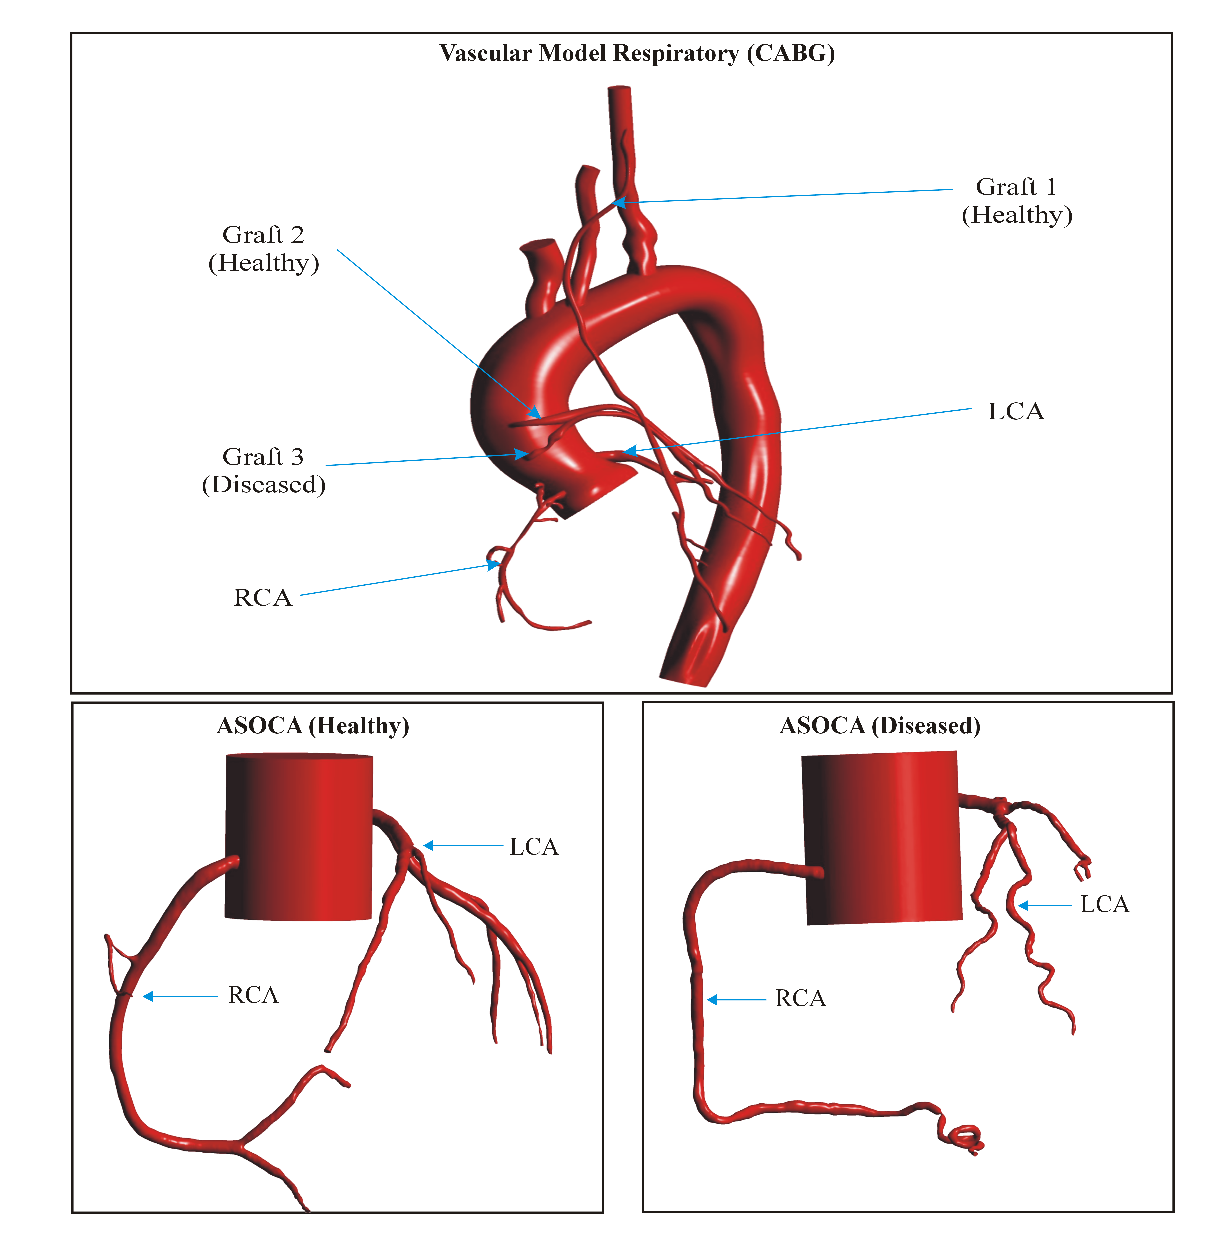
\includegraphics[width=0.91\textwidth]{Sample (2).pdf}
   \caption{Healthy and diseased coronary artery and bypass graft models from the Vascular Model Repository and ASOCA datasets, including CABG geometries and ASOCA coronary arteries with an artificially added ascending aorta.}

         \label{fig:1}
     \end{figure}

\begin{table}[h!]
\centering
    \setlength{\tabcolsep}{2.9pt}
    \renewcommand{\arraystretch}{0.9}
    \caption{The inlet diameters of healthy coronary arteries, bypass grafts, and diseased coronary arteries from both datasets (Vascular Model Respiratory and ASCOA), along with the volumetric flow rates (mL/s) for each vessel under both the Newtonian and Carreau-Yasuda models.}
    \begin{tabular}{|c|c|c|c|c|c|c|c|c|c|c|c|c|c|c|c|c|c|c|c|c|c|c|c|c|c|} 
    \hline 
    \multirow{2}{*}{\textbf{Models}} & \multicolumn{4}{c|}{Healthy (H)} & \multicolumn{5}{c|}{Bypass Grafts (BG)} &\multicolumn{3}{c|}{Diseased (D)} \\ \cline{2-13} & H1 & H2 & H3 & H4 & BG1 & BG2 & BG3 & BG4 & BG5 & D1 & D2 & D3 \\ \hline
  \textbf{Inlet Diameter (cm)}& 3.1 & 3.4 & 3.4 & 3.4& 3.14 & 4.1 & 3 & 4 & 3.2 & 3.4 &3.4& 3.4  \\ \hline \multicolumn{13}{|c|}{\textbf{Newtonian Model}}\\ \hline  \textbf{Inlet}& 76.1 & 90.8 & 90.8 & 90.7& 77.8 & 131.9 & 70.6 & 125.6 & 80.2 & 90.7 &90.7& 90.6  \\ \hline  \textbf{RCA}& 1.3 & 0.8 & 0.6 & 0.8& 0.6 & 1.3 & 0.3 & 1.3 & 0.9 & 0.6 &0.5& 0.5  \\ \hline  \textbf{LCA}& 1.7 & 2.8 & 1.3 & 1.2& - & 1.3 & 1.3 & 1.2 & 2.5 & 1.2 &1.4& 2.5  \\ \hline 
   \textbf{Graft 1 (H)}& - & - & - & -& 1.3 & 0.5 & 0.7 & 0.8 & 0.6 & - &-& -  \\ \hline 
   \textbf{Graft 2 (H)}& - & - & - & -& 0.7 & 1.2 & 0.8 & 0.5 & 0.6 & - &-& - \\ \hline 
   \textbf{Graft 3 (D)}& - & - & - & -& 0.6 & 1.1 & 0.9 & 0.5 & 0.5 & - &-& - \\ \hline 
   \multicolumn{13}{|c|}{\textbf{Carreau-Yasuda Model}}\\ \hline  \textbf{Inlet}& 76.1 & 90.8 & 90.8 & 90.7& 77.8 & 126.7 & 70.5 & 125.6 & 80.2 & 90.7 &90.7& 90.6  \\ \hline  \textbf{RCA}& 1.2 & 0.7 & 0.7 & 0.6& 0.6 & 1.3 & 0.3 & 1.3 & 0.9 & 0.6 &0.6& 0.6  \\ \hline  \textbf{LCA}& 1.6 & 2.3 & 1.1 & 1.2& - & 1.3 & 1.3 & 1.2 & 2.6 & 1.6 &1.2& 2.2  \\ \hline 
   \textbf{Graft 1 (H)}& - & - & - & -& 1.2 & 0.4 & 0.7 & 0.8 & 0.6 & - &-& -  \\ \hline 
   \textbf{Graft 2 (H)}& - & - & - & -& 0.6 & 1.2 & 0.8 & 0.5 & 0.6 & - &-& - \\ \hline 
   \textbf{Graft 3 (D)}& - & - & - & -& 0.5 & 1.0 & 0.9 & 0.5 & 0.5 & - &-& - 
    \\ \hline
       \end{tabular}
    \label{tab:a}
\end{table}


\subsection{\label{sec:governing_equations}Governing Equations and Numerical Modeling} 

\hspace*{\parindent} The incompressible Navier-Stokes equations were employed to effectively characterize the flow behavior \cite{6}:
\begin{align}\label{eq:continuity}
\vec{\nabla} \cdot \vec{v} = 0,
\end{align}
\begin{align}\label{eq:navier_stokes}
\rho (\vec{v} \cdot \vec{\nabla}) \vec{v} = -\vec{\nabla} p + \mu \nabla^2 \vec{v},
\end{align} 
where $\rho$ denotes density and $\mu$ represents dynamic viscosity.

Blood, composed of cells suspended in plasma, demonstrates non-Newtonian behavior, particularly notable in vessels with diameters smaller than 1 mm. Under certain pathological and transient conditions, such as artery dilation and bifurcations, shear rates may decrease below \(100 \, \text{s}^{-1}\), emphasizing the potential importance of non-Newtonian processes \cite{7, 29, 30}. Conversely, in larger blood vessels, where shear rates typically exceed \(100 \, \text{s}^{-1}\) and with diameters exceeding 0.3 mm, blood can be accurately represented as a Newtonian fluid \cite{26, 27}. In our current study, we compare two viscosity models, the Newtonian model and the non-Newtonian Carreau-Yasuda model.

For the non-Newtonian Carreau-Yasuda model \cite{32}, the viscosity $\mu(\dot{\gamma})$ is given by:

\begin{equation}
\mu(\dot{\gamma}) = \mu_{\infty} + (\mu_0 - \mu_{\infty}) \left(1 + (\lambda\dot{\gamma})^a \right)^{\frac{n-1}{a}},
\end{equation}
where \(\dot{\gamma}\) is a scalar measure of the rate of deformation tensor \(D = [\nabla \mathbf{U} + (\nabla \mathbf{U})^T]/{2}\) (s\(^{-1}\)), defined as \(\dot{\gamma} = \sqrt{2 \, \text{tr}(D^2)}\) (s\(^{-1}\)), and the parameters are: $\mu_{\infty} = 0.0035$ Pa-s, $\mu_0 = 0.16$ Pa-s, $\lambda = 8.2$ s, $n = 0.2128$, and $a = 0.64$.

The Carreau-Yasuda model is widely used for numerical simulation of shear-thinning blood behaviour  \cite{80,81}. This model was developed in order to more accurately describe the mechanical properties of blood, given its complex composition and behavior \cite{82}. The Carreau-Yasuda model takes into account the interaction of blood components (plasma, red blood cells, white blood cells, platelets), making it possible to reproduce physical properties more accurately. So, it can serve as an alternative to multi-phase models applied in cardiovascular simulations \cite{83}. Moreover, this model can describe such nonlinear characteristics, making it useful for analyzing blood flow under various conditions \cite{84} and capture shear-thinning effects, which blood exhibits in large and medium vessels \cite{85,86}. In addition, it can be easily implemented into commercial or open-source software \cite{87}.

Additionally, the  Newtonian blood model was adopted. Blood density was equal to 1,050 kg/m$^3$ and viscosity of 0.0035 Pa-s \cite{9}. 

A uniform velocity of 10 cm/s is applied at the inlet for all models, ensuring laminar flow. Consistent with published data \cite{2}, 4\% of the inlet flow is directed to the coronary circulation. To achieve the desired volumetric flow rates, pressure outlet boundary conditions or mass flow conditions are applied at the outlets of both coronary arteries and grafts. The inlet diameters and volumetric flow rates are detailed in Table \ref{tab:a} \cite{3}. It should be clarified that we did not consider the systolic and diastolic phases of the heart contraction and actual coronary flow rates will oscillate depending on the cardiac cycle and coronary flow will be higher during the diastolic phase, as the heart muscle relaxes to decrease the resistance along its arteries \cite{70, 71}.

In simulations, the rigid arterial walls are considered for simplicity when calculating WSS, and the no-slip condition is applied. The WSS for vessels \cite{78} can be calculated using the formula:

\begin{align}
    \tau_w = \mu \frac{\partial v}{\partial n} \bigg|_{n=0},
\end{align}

    where \( \mu \) is the blood viscosity, \( \frac{\partial v}{\partial n} \) is the velocity gradient in the direction \(n\) normal to the wall.

\subsection{\label{CFD Simulation}CFD Simulation} 
\hspace*{\parindent}The governing equations are solved using the ANSYS Fluent commercial solver, which utilizes the finite volume method. In this methodology, the pressure-based solver is employed to systematically solve the non-linear equations of mass and momentum conservation. In order to achieve precise convergence, a threshold for residual error convergence is established at \(10^{-3}\) to \(10^{-4}\). Following a mesh independence study, an optimal mesh size for the coronary arteries and bypass grafts was determined to range between 0.3 mm and 0.4 mm. Various mesh sizes were tested, and this range was selected when negligible differences in observed WSS were observed, depending on the specific model being analyzed.

\subsection{\label{Statistical Analysis}Statistical Analysis}\hspace*{\parindent}Statistical analysis was performed to evaluate several critical variables related to WSS in various vessels. For CAD patients without CABG, both right and left coronary artery measurements are reported. For CABG patients, right and left coronary artery measurements were reported as long as they were functional either spontaneously or with by-passed grafts. Right or left coronary artery measurements were omitted if they were totally blocked and were not functional for distal myocardial supply. 

In this study, elevated WSS was noted at the outlets of some coronary artery and grafts. To enhance the accuracy of the analysis, we clipped 1 to 2 cm from the outlet regions of models where high WSS was detected. This clipping was performed to mitigate boundary effects and to focus on areas that more accurately represent physiological flow conditions. By excluding segments that could exhibit flow features due to end effects (at the outlets), we aimed to improve the quality and reliability of the data, leading to more precise interpretations of WSS distributions in the coronary arteries and grafts. 

The computed variables included the area-weighted average WSS, average WSS at bifurcations, the area fraction (defined as the ratio of the vessel area where WSS exceeds 40 dynes/cm$^2$ to the total vessel area), the proportion of WSS values exceeding 40 dynes/cm$^2$, and the interquartile range (IQR) of WSS. To determine statistical significance, the Mann-Whitney U test was employed to compare measured parameters of coronary arteries from healthy controls with CAD patients (with or without CABG surgery)  and healthy grafts (HG) with diseased grafts (DG) of CABG surgery. This non-parametric test was chosen due to its suitability for comparing distributions between two independent groups, particularly when the data does not follow a normal distribution or when sample sizes are small. A significance threshold of $p < 0.05$ was applied, with results meeting this criterion reported as statistically significant, while those not meeting the threshold were marked as \textit{ns} (non-significant).


To further investigate associations between flow-related parameters and wall shear stress, a correlation analysis was performed between key hemodynamic variables, including inlet diameter, inlet velocity, RCA and LCA flow rates, and flow rates in healthy and diseased grafts, and the corresponding WSS metrics. Pearson correlation matrices were computed for both the Newtonian and non-Newtonian (Carreau--Yasuda) models using
\begin{equation}\label{eq:pearson}
\addp{r = \frac{\sum_i (x_i - \bar{x})(y_i - \bar{y})}{\bigl[\sum_i (x_i - \bar{x})^2\bigr]^{1/2}\,\bigl[\sum_i (y_i - \bar{y})^2\bigr]^{1/2}}},
\end{equation}
where \(x_i\) and \(y_i\) denote individual variable values and \(\bar{x}\) and \(\bar{y}\) represent their mean values\addp{; the denominator is the product of the two independent sample standard deviations}. Correlation strength was classified as weak (\(|r| < 0.3\)), moderate (\(0.3 \le |r| < 0.7\)), or strong (\(|r| \ge 0.7\)). The resulting correlation matrices were visualized as heat maps and statistical significance was assessed using a threshold of \(p < 0.05\). In total, twelve models (four healthy coronary arteries, five grafts, and three diseased coronary arteries) were analyzed, with data grouped into healthy controls, CABG patients, and diseased grafts, consistent with the statistical comparisons described above.


\subsection{\label{PINN Methodology}{Physics-Informed Neural Network Surrogate Model}}
{

\hspace*{\parindent}Traditional CFD simulations, while highly accurate, require substantial computational resources and time for mesh generation, solver configuration, and iterative convergence \cite{57}. Each simulation can take several hours to complete, making it impractical to perform the multiple simulations needed for parametric studies or surgical planning scenarios. To address this limitation, we developed PINNs as surrogate models that can predict hemodynamic quantities with accuracy comparable to CFD but at a fraction of the computational cost \cite{92, 94}. PINNs are mesh-free and naturally handle inverse problems or assimilate sparse data, as they learn solutions that are continuous in space and time while satisfying physical constraints \cite{89}. Unlike traditional CFD, PINNs operate directly on spatial coordinates, eliminating the need for discretization and making them particularly suitable for complex patient-specific geometries. Once trained, a PINN can replace expensive iterative CFD solutions with fast neural network evaluations, reducing prediction times from hours to seconds and representing an important step towards enabling patient-specific blood flow analysis in clinical decision-making \cite{94}. The PINN framework combines supervised learning on CFD data with physics-based regularization derived from the Navier-Stokes equations, ensuring that predictions remain physically consistent even in regions with sparse training data \cite{93}.

{In recent studies of blood flow in aortic and arterial aneurysms, PINN models reproduced velocity, pressure, and WSS distributions in strong agreement with high-fidelity CFD while requiring only a fraction of the computational cost \cite{92, 94}. Similarly, Arzani et al. (2021) showed that a PINN can accurately recover near-wall flow features and WSS in diseased arteries even when only a few sparse velocity measurements away from the wall are available \cite{93}. In coronary flow applications, PINN-based surrogates have likewise reached high fidelity. For example, a 1D PINN was used to provide boundary conditions in a coronary tree FSI simulation. When validated against traditional CFD, it yielded strong accuracy while inherently enforcing fundamental flow physics \cite{95}. Wang et al. (2025) proposed a transductive PINN (T-PINN) that incorporates governing equations even for test-case geometries, which yielded improved performance on unseen cardiovascular flow scenarios compared to standard neural network surrogates trained only on data \cite{97}. \addp{Reduced-order data-driven surrogates form a parallel and complementary line of work. Barzegar Gerdroodbary and Salavatidezfouli have applied proper orthogonal decomposition (POD) coupled with long short-term memory (LSTM) networks to predict patient-specific carotid artery stenosis haemodynamics~\cite{108}. The same authors have also compared linear (POD--LSTM) and nonlinear (CNN--LSTM) solution-manifold reductions in cardiovascular fluid--structure interaction~\cite{109}. Rajhi et al.~\cite{110} combine POD with machine learning to predict cerebral saccular aneurysm flow under a non-Newtonian (Casson) rheology. These surrogates achieve large speed-ups by projecting onto a reduced basis but require dense supervised data for the basis construction. The PINN approach used here is structurally different in two ways relevant to WSS prediction. First, the embedded Navier--Stokes residual provides a physics regulariser that constrains predictions in low-data regions such as near the walls of stenoses. Second, PINN inference is mesh-free, predicting at arbitrary spatial coordinates without re-projection onto a reduced basis.}}   

The neural network $\mathcal{N}_\theta: \mathbb{R}^3 \rightarrow \mathbb{R}^5$ maps spatial coordinates $(x, y, z)$ to hemodynamic quantities $(u, v, w, p, \tau_w)$, where $u, v, w$ represent the velocity components in the $x$, $y$, and $z$ directions, $p$ is the pressure field, and $\tau_w$ denotes the WSS magnitude. \replaced[id=pinn]{The architecture is chosen to resolve the steep WSS gradients that develop at bifurcations, stenotic regions, and high-curvature segments.}{The network architecture is designed to capture the complex spatial variations in WSS that occur at bifurcations, stenotic regions, and vessel curvatures, where the flow exhibits steep gradients and localized high-stress zones.}

{\subsubsection{Network Architecture}}
Standard multilayer perceptrons suffer from spectral bias, meaning that they tend to learn low-frequency components of the target function more readily than high-frequency features \cite{89}. This presents a significant challenge for the prediction of WSS in coronary arteries and grafts, where the flow field contains smooth regions along straight vessel segments and sharp gradients at bifurcations, stenoses, and anastomosis sites. To address this limitation, we adopt Fourier feature encoding \cite{90}, which maps the input coordinates into a higher-dimensional feature space, thereby enabling the network to represent and learn high-frequency components with greater efficacy. The encoding function is defined as:
\begin{equation}
    \gamma(\mathbf{x}) = \left[ \mathbf{x}, \sin(2\pi \mathbf{B} \mathbf{x}), \cos(2\pi \mathbf{B} \mathbf{x}) \right]
\end{equation}
Here, $\mathbf{x} = (x, y, z)$ denotes the three-dimensional input coordinates, and $\mathbf{B} \in \mathbb{R}^{m \times 3}$ is a matrix of random Fourier frequencies whose entries are sampled from a Gaussian distribution with standard deviation $\sigma = 10$. In our configuration, we set $m = 64$ frequency components, which yields an encoded feature vector of dimensionality $(3 + 2 \times 64) = 131$. The random Fourier features function as a learnable basis that spans a broad spectrum of spatial frequencies, thereby enabling the network to represent both the slowly varying distributions of WSS along vascular surfaces and the pronounced local gradients arising at geometric irregularities.

The overall architecture of the PINN is depicted in Figure \ref{fig:pinn_arch}. The encoded feature vector is subsequently propagated through a trunk network composed of {6} residual blocks \cite{100,99}. Each residual block contains two linear layers with {48} hidden units, separated by SiLU (Sigmoid Linear Unit) activation functions. The residual connections facilitate gradient flow during backpropagation and enable the training of deeper networks. The input layer uses a learnable Swish activation function $f(x) = x \cdot \sigma(\beta x)$, where $\beta$ is a trainable parameter initialized to 1.0, allowing the network to adapt the activation shape during training. The trunk network projects to five separate output heads that produce the velocity components $(u, v, w)$, pressure $p$, and WSS $\tau_w$. This multi-output architecture allows the network to simultaneously learn all relevant hemodynamic quantities while sharing learned representations. The network contains approximately {34,000} trainable parameters, which allows efficient training on a single GPU. {Network parameters are initialized using the Xavier uniform initialization \cite{91} with bias terms set to zero.} \addp{The architecture is exercised on two distinct sets of points, reflecting the dual data-and-physics nature of the loss. The data losses $\mathcal{L}_{\text{wss}}$ and $\mathcal{L}_{\text{vel}}$ are evaluated on supervised CFD points: wall-surface points carry the WSS magnitude $\tau_w$ (which is defined only on the wall) and interior streamline samples carry the velocity components $u, v, w$. The physics losses $\mathcal{L}_{\text{NS}}$, $\mathcal{L}_{\text{cont}}$, and $\mathcal{L}_{\tau}$ are instead evaluated on collocation points drawn from the fluid domain, where the Navier--Stokes momentum and continuity residuals must vanish for any physically valid solution. The spatial derivatives of $u, v, w, p$ entering these residuals, and the wall-tangential velocity gradient $\partial u_t/\partial n$ entering the WSS-from-gradient consistency, are obtained by automatic differentiation through the trunk network. This separation between supervised data points (where ground-truth values are available) and unsupervised collocation points (where the governing equations are enforced) is what distinguishes the present surrogate from a purely data-driven regressor and is the source of its physics-informed regularisation in regions of sparse coverage, such as the immediate near-wall layer of a stenosis.}
}

\begin{figure}
\centering
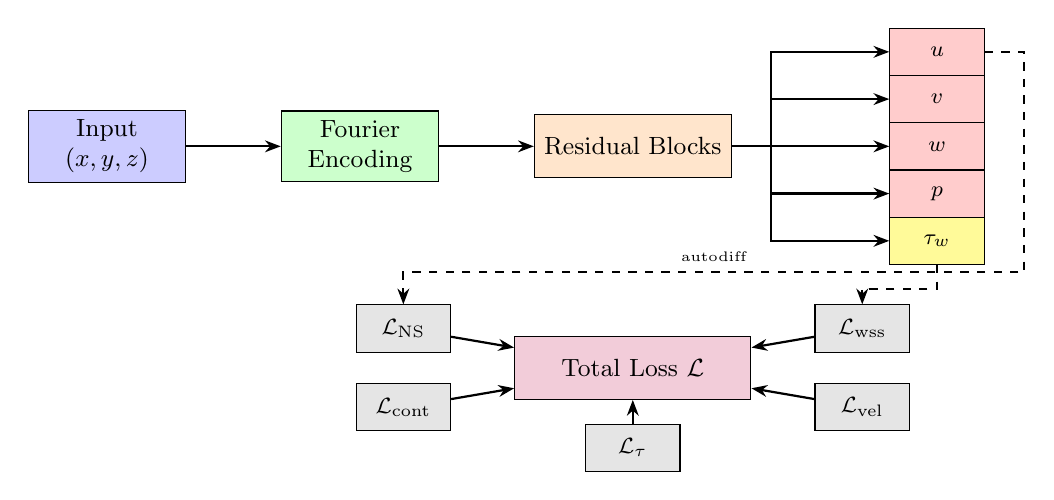
\begin{tikzpicture}[
    node distance=0.8cm and 1.2cm,
    box/.style={rectangle, draw, minimum width=2cm, minimum height=0.8cm, align=center, font=\small},
    smallbox/.style={rectangle, draw, minimum width=1.2cm, minimum height=0.6cm, align=center, font=\footnotesize},
    arrow/.style={-{Stealth[length=2mm]}, thick},
    label/.style={font=\footnotesize}
]

% Input
\node[box, fill=blue!20] (input) {Input\\$(x, y, z)$};

% Fourier Encoding
\node[box, fill=green!20, right=of input] (fourier) {Fourier\\Encoding};

% Residual Blocks
\node[box, fill=orange!20, right=of fourier, minimum width=2.5cm] (resblocks) {Residual Blocks};

% Output heads
\node[smallbox, fill=red!20, right=2cm of resblocks, yshift=1.2cm] (u) {$u$};
\node[smallbox, fill=red!20, right=2cm of resblocks, yshift=0.6cm] (v) {$v$};
\node[smallbox, fill=red!20, right=2cm of resblocks, yshift=0cm] (w) {$w$};
\node[smallbox, fill=red!20, right=2cm of resblocks, yshift=-0.6cm] (p) {$p$};
\node[smallbox, fill=yellow!40, right=2cm of resblocks, yshift=-1.2cm] (wss) {$\tau_w$};

% Arrows
\draw[arrow] (input) -- (fourier);
\draw[arrow] (fourier) -- (resblocks);
\draw[arrow] (resblocks.east) -- ++(0.5,0) |- (u.west);
\draw[arrow] (resblocks.east) -- ++(0.5,0) |- (v.west);
\draw[arrow] (resblocks.east) -- ++(0.5,0) |- (w.west);
\draw[arrow] (resblocks.east) -- ++(0.5,0) |- (p.west);
\draw[arrow] (resblocks.east) -- ++(0.5,0) |- (wss.west);

% Loss connections
\node[box, fill=purple!20, below=2cm of resblocks, minimum width=3cm] (loss) {Total Loss $\mathcal{L}$};

% Physics and Data loss boxes (5 total)
\node[smallbox, fill=gray!20, left=0.8cm of loss, yshift=0.5cm] (lns) {$\mathcal{L}_{\text{NS}}$};
\node[smallbox, fill=gray!20, left=0.8cm of loss, yshift=-0.5cm] (lcont) {$\mathcal{L}_{\text{cont}}$};
\node[smallbox, fill=gray!20, right=0.8cm of loss, yshift=0.5cm] (lwss) {$\mathcal{L}_{\text{wss}}$};
\node[smallbox, fill=gray!20, right=0.8cm of loss, yshift=-0.5cm] (lvel) {$\mathcal{L}_{\text{vel}}$};
\node[smallbox, fill=gray!20, below=0.3cm of loss] (ltau) {$\mathcal{L}_{\tau}$};

% Loss arrows
\draw[arrow] (lns) -- (loss);
\draw[arrow] (lcont) -- (loss);
\draw[arrow] (lwss) -- (loss);
\draw[arrow] (lvel) -- (loss);
\draw[arrow] (ltau) -- (loss);

% Autodiff arrows - showing automatic differentiation from outputs to physics loss
\draw[arrow, dashed] (u.east) -- ++(0.5,0) -- ++(0,-2.8) -| (lns.north) node[near start, above, font=\tiny] {autodiff};
\draw[arrow, dashed] (wss.south) -- ++(0,-0.3) -| (lwss.north);

\end{tikzpicture}
\caption{FourierPINN surrogate for WSS prediction. Input coordinates $(x,y,z)$ pass through the Fourier feature map, a trunk of 6 residual blocks (\addp{detailed in Figure~\ref{fig:pinn_resblock}}), and five output heads $u,v,w,p,\tau_w$. The five loss components $\mathcal{L}_{\text{wss}}$, $\mathcal{L}_{\text{vel}}$, $\mathcal{L}_{\text{NS}}$, $\mathcal{L}_{\text{cont}}$, $\mathcal{L}_\tau$ are aggregated into the total loss $\mathcal{L}$; the dashed arrow labelled \emph{autodiff} marks where the spatial derivatives feeding the physics losses are obtained by automatic differentiation through the trunk.}
\label{fig:pinn_arch}
\end{figure}

\begin{figure}[htbp]
\centering
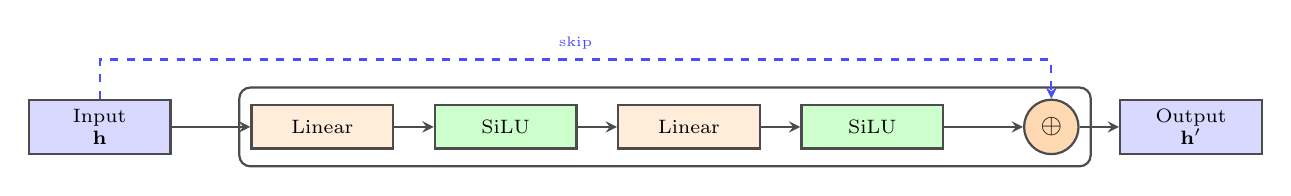
\begin{tikzpicture}[
    node distance=0.5cm,
    layer/.style={rectangle, draw=black!70, thick, minimum width=1.8cm, minimum height=0.55cm, align=center, font=\scriptsize},
    box/.style={rectangle, draw=black!70, thick, rounded corners, inner sep=4pt},
    arrow/.style={->, >=stealth, thick, color=black!70},
    skip/.style={->, >=stealth, thick, dashed, color=blue!70}
]

% Residual Block Structure (horizontal)
\node[layer, fill=blue!15] (input) {Input\\$\mathbf{h}$};
\node[layer, fill=orange!15, right=1cm of input] (linear1) {Linear};
\node[layer, fill=green!20, right=of linear1] (act1) {SiLU};
\node[layer, fill=orange!15, right=of act1] (linear2) {Linear};
\node[layer, fill=green!20, right=of linear2] (act2) {SiLU};
\node[circle, draw=black!70, thick, fill=orange!30, right=1cm of act2, minimum size=0.6cm, font=\normalsize] (add) {$\oplus$};
\node[layer, fill=blue!15, right=0.5cm of add] (output) {Output\\$\mathbf{h}'$};

% Bounding box
\node[box, fit=(linear1)(act1)(linear2)(act2)(add)] {};

% Main flow
\draw[arrow] (input) -- (linear1);
\draw[arrow] (linear1) -- (act1);
\draw[arrow] (act1) -- (linear2);
\draw[arrow] (linear2) -- (act2);
\draw[arrow] (act2) -- (add);
\draw[arrow] (add) -- (output);

% Skip connection
\draw[skip] (input.north) -- ++(0,0.5) -| node[pos=0.25, above, font=\tiny] {skip} (add.north);
\end{tikzpicture}
\caption{Residual block architecture. Each block contains two linear layers with 48 hidden units and SiLU activations, with a skip connection adding the input directly to the output.}
\label{fig:pinn_resblock}
\end{figure}


{
{\subsubsection{Loss Function}}
The training objective for the PINN combines data-driven supervision from CFD results with physics-based regularization derived from the steady incompressible Navier-Stokes equations in non-dimensional form. The total loss comprises five components: (1) wall shear stress data fidelity, (2) velocity data fidelity, (3) momentum equation residuals, (4) continuity (mass conservation) constraints, and (5) WSS physics consistency ($\tau = \mu \partial u_t / \partial n$). This physics-informed approach ensures that the network not only fits the training data but also satisfies the governing equations of fluid flow throughout the computational domain. The total loss function is defined as a weighted sum of these five components:
\begin{equation}
    \mathcal{L} = \lambda_{\text{wss}} \mathcal{L}_{\text{wss}} + \lambda_{\text{vel}} \mathcal{L}_{\text{vel}} + \lambda_{\text{NS}} \mathcal{L}_{\text{NS}} + \lambda_{\text{cont}} \mathcal{L}_{\text{cont}} {+ \lambda_{\tau} \mathcal{L}_{\tau}}
\end{equation}
\addp{where $\lambda_{\text{wss}}, \lambda_{\text{vel}}, \lambda_{\text{NS}}, \lambda_{\text{cont}}, \lambda_{\tau}$ are weighting coefficients. These are not fixed hyperparameters; they are derived once per patient at the start of training by gradient-norm balancing, with a small clinical-priority factor that emphasises WSS prediction. The full procedure is described in the Training Procedure subsection.}

The first data loss term enforces agreement between predicted and CFD-computed WSS values at wall boundary points. \addp{This term receives the highest clinical-priority factor in the balancing scheme, reflecting the role of WSS in identifying high-risk plaque regions.} The WSS loss is computed as:
\begin{equation}
    \mathcal{L}_{\text{wss}} = \frac{1}{N_{\text{wall}}} \sum_{i=1}^{N_{\text{wall}}} |\tau_{w,i}^{\text{pred}} - \tau_{w,i}^{\text{CFD}}|^2
\end{equation}
where $N_{\text{wall}}$ denotes the number of points on the surface of the vessel wall, and $\tau_{w,i}^{\text{pred}}$ and $\tau_{w,i}^{\text{CFD}}$ represent the predicted and ground-truth WSS values, respectively.

The second data loss term ensures accurate reconstruction of the velocity field throughout the computational domain, including both wall surfaces and interior streamline locations. Although velocity prediction is not the primary clinical objective, accurate velocity fields are necessary to calculate physically consistent pressure distributions and WSS values through momentum equations. The velocity loss is defined as:
\begin{equation}
    \mathcal{L}_{\text{vel}} = \frac{1}{N} \sum_{i=1}^{N} \|\mathbf{u}_i^{\text{pred}} - \mathbf{u}_i^{\text{CFD}}\|^2
\end{equation}
where $N$ is the total number of sampled points from the CFD mesh, and $\mathbf{u}_i = (u_i, v_i, w_i)$ represents the velocity vector at location $i$.

\replaced[id=pinn]{In addition to the data-driven loss terms, we incorporate physics-based regularisation that enforces the governing equations of fluid dynamics. This is what distinguishes a PINN from a purely data-driven regressor and brings two practical benefits. First, the embedded constraints act as a regulariser that constrains predictions in regions where supervised data are sparse, such as the immediate near-wall layer of a stenosis, reducing the network's tendency to fit noise rather than physics. Second, the physics loss enforces conservation of mass and momentum at every collocation point, ensuring that predicted velocity and pressure fields are not merely accurate in a least-squares sense but also internally consistent, which matters for downstream quantities such as WSS that are computed from the gradients of these fields.}{In addition to the data-driven loss terms, we incorporate physics-based regularization that enforces the governing equations of fluid dynamics. This approach distinguishes PINNs from purely data-driven machine learning models and provides several advantages. First, the embedded physical constraints act as a strong regularizer that prevents overfitting and enables accurate predictions even when extrapolating beyond the training data distribution. Second, the physics loss ensures that predictions satisfy fundamental conservation laws for mass and momentum, which is critical for clinical applications where non-physical predictions could lead to incorrect assessments of hemodynamic risk.}

The physics loss enforces the steady-state incompressible Navier-Stokes momentum equations at collocation points sampled throughout the computational domain. For incompressible Newtonian flow, the momentum equation in the $x$-direction is given by:
\begin{align}
    f_u &= \rho\left(u\frac{\partial u}{\partial x} + v\frac{\partial u}{\partial y} + w\frac{\partial u}{\partial z}\right) + \frac{\partial p}{\partial x} - \mu\left(\frac{\partial^2 u}{\partial x^2} + \frac{\partial^2 u}{\partial y^2} + \frac{\partial^2 u}{\partial z^2}\right)
\end{align}
where $\rho$ is the blood density, $\mu$ is the dynamic viscosity, and $f_u$ represents the momentum residual. For a solution that exactly satisfies the Navier-Stokes equations, this residual would be zero at all points in the domain. Similar expressions are derived for the momentum components $y$ and $z$, resulting in residuals $f_v$ and $f_w$. All spatial derivatives appearing in these expressions are computed using automatic differentiation through the neural network, which provides exact gradients of the network outputs with respect to the input coordinates. The blood properties used in the physics loss are $\rho = {1050}$ kg/m$^3$ and $\mu = 0.0035$ Pa$\cdot$s, matching the values employed in the CFD simulations to ensure consistency between the surrogate model and the ground truth data. The Navier-Stokes loss is defined as the mean squared residual:
\begin{equation}
    \mathcal{L}_{\text{NS}} = \frac{1}{N_c} \sum_{i=1}^{N_c} \left( f_u^2 + f_v^2 + f_w^2 \right)
\end{equation}
where $N_c$ denotes the number of collocation points at which the momentum equations are enforced.

Mass conservation for incompressible flow requires that the divergence of the velocity field vanishes throughout the domain. This continuity constraint is expressed as:
\begin{equation}
    \mathcal{L}_{\text{cont}} = \frac{1}{N_c} \sum_{i=1}^{N_c} \left( \frac{\partial u}{\partial x} + \frac{\partial v}{\partial y} + \frac{\partial w}{\partial z} \right)^2
\end{equation}
By minimizing this loss term, the network learns to predict velocity fields that are divergence-free, ensuring that mass is conserved locally at every point in the domain.

\replaced[id=pinn]{The fifth loss term enforces consistency between the predicted WSS head $\tau_w^{\text{pred}}$ and the WSS implied by the wall-normal velocity gradient at the same wall point:}{The fifth loss term enforces physical consistency between the predicted WSS and the velocity gradients at wall surfaces. Since WSS is fundamentally derived from the wall-normal velocity gradient, we include an additional constraint:}
{\begin{equation}
    \mathcal{L}_{\tau} = \frac{1}{N_{\text{wall}}} \sum_{i=1}^{N_{\text{wall}}} \left| \tau_{w,i}^{\text{pred}} - \mu \left. \frac{\partial u_t}{\partial n} \right|_i \right|^2
\end{equation}}
{where $u_t$ is the tangential velocity component and $n$ is the wall-normal direction. Surface normal vectors at wall points were estimated from the point cloud geometry using k-nearest neighbor analysis ($k=30$) via the Open3D library, with normals consistently oriented toward the vessel centre. This constraint ensures that the network's direct WSS predictions are consistent with the velocity field gradients computed via automatic differentiation, preventing physically inconsistent solutions. Together with the momentum and continuity equations, this provides a complete set of physics constraints that guide the network toward physically realistic solutions.}

\addp{We train both a Newtonian and a Carreau--Yasuda PINN surrogate for every patient. The Newtonian surrogate is trained against the Newtonian CFD targets using the constant-viscosity momentum residual and WSS-from-gradient consistency introduced above. The constant viscosity $\mu = 0.0035$~Pa$\cdot$s appears identically in the data targets and in the physics-loss residual. The Carreau--Yasuda surrogate is trained against the Carreau--Yasuda CFD targets using a non-Newtonian variant of the same physics losses. In this variant the effective viscosity $\mu_{\mathrm{eff}}(\dot\gamma)$ is evaluated pointwise from the local strain-rate tensor of the predicted velocity field via the Carreau--Yasuda closure of Section~\ref{Geometric Description}. The local shear rate is computed by automatic differentiation as $\dot\gamma = \sqrt{2\,D_{ij}D_{ij}}$ with $D_{ij}=\tfrac{1}{2}(\partial_i u_j+\partial_j u_i)$. Each surrogate is therefore trained against governing equations consistent with its training data, eliminating the rheology mismatch identified by the Editor. The two pipelines share the same FourierPINN architecture and training procedure (Algorithm~\ref{alg:pinn_train}). Only the viscosity that enters the physics loss differs between them. The accuracy of both surrogates is reported per patient in Tables~\ref{tab:pinn_holdout} (Newtonian) and~\ref{tab:pinn_holdout_cy} (Carreau--Yasuda) for all twelve patients.}

{\subsubsection{Training Procedure}}
\replaced[id=pinn]{Boundary conditions are imposed implicitly through the training data rather than as hard constraints. The interior streamline samples used by $\mathcal{L}_{\text{vel}}$ are drawn from a CFD simulation in which no-slip, inlet, and outlet conditions were already enforced; the surrogate therefore learns velocity fields that are consistent with those boundary conditions wherever the data densely covers the lumen, and the wall surface points used by $\mathcal{L}_{\text{wss}}$ supervise WSS at exactly the locations where no-slip would be applied. This avoids explicit encoding of boundary conditions, which would be cumbersome for complex patient-specific geometries with multiple inlets, outlets and graft anastomoses.}{The PINN formulation incorporates boundary conditions implicitly through the training data. For steady-state incompressible flow, the no-slip condition ($\mathbf{u} = 0$) at vessel walls is enforced by supervised learning on CFD wall surface points with corresponding WSS ground truth. Inlet velocity profiles and outlet pressure conditions from the CFD simulations are similarly learned from the training data, avoiding explicit encoding that would be cumbersome for complex patient-specific geometries with multiple boundaries.}

Prior to training, the CFD mesh coordinates and solution fields were exported and preprocessed to facilitate neural network optimization. {We employ a physics-based non-dimensional formulation where spatial coordinates are uniformly scaled using a single reference length $L_{\text{ref}}$ equal to the maximum coordinate range across all dimensions. This uniform scaling preserves the geometric aspect ratio of the vessel, which is critical for thin tubular coronary arteries where non-uniform scaling would distort the physics. The scaled coordinates $\mathbf{x}^* = (\mathbf{x} - \mathbf{x}_{\text{min}}) / L_{\text{ref}}$ lie in $[0, 1]^3$ while maintaining proper spatial relationships. Velocities are scaled by a reference velocity $U_{\text{ref}}$ taken as the 95th percentile of the velocity magnitude in the CFD data (a robust upper bound that avoids inflation by isolated extrema), yielding non-dimensional velocities $\mathbf{u}^* = \mathbf{u} / U_{\text{ref}}$. WSS is scaled by a data-driven reference $T_{\text{ref}}$ (95th percentile of WSS values) to ensure network outputs remain $O(1)$, improving training stability.} This normalization ensures that all network outputs operate in similar numerical ranges while the physics loss is evaluated in non-dimensional form using the Reynolds number $\text{Re} = \rho U_{\text{ref}} L_{\text{ref}} / \mu$.

{While PINNs are inherently meshless at inference, capable of predicting hemodynamic quantities at arbitrary spatial coordinates without requiring mesh generation, the training process requires collocation points to lie within the fluid domain where the governing equations apply.} Collocation points for physics loss evaluation were sampled directly from the CFD mesh rather than from a uniform random distribution over the bounding box. This sampling strategy is critical for coronary artery geometries, which consist of thin tubular structures with typical diameters of 3--5 mm embedded within bounding boxes spanning several centimeters in each dimension. Uniform sampling would place the vast majority of collocation points in the empty space surrounding the vessels, where the Navier-Stokes equations are not applicable. By sampling from the CFD mesh, we ensure that all collocation points lie within the fluid domain where the physics constraints are meaningful. Furthermore, during collocation sampling, interior points (from streamline data) were assigned higher sampling probability than wall surface points, as interior points have non-zero velocities and provide more informative gradients for the Navier-Stokes residuals. This weighted sampling strategy concentrates the physics loss evaluation in regions where the flow field exhibits non-trivial behaviour.

The network was trained using the AdamW optimizer with weight decay regularization of $10^{-5}$ to prevent overfitting. The initial learning rate was set to {$2 \times 10^{-4}$} and gradually reduced following a cosine annealing schedule over the course of training. This schedule allows for rapid initial convergence while fine-tuning the solution in later epochs. Each training iteration used a batch size of {8,192} data points sampled randomly from the complete CFD dataset for that patient, along with {4,096} collocation points for evaluating the physics loss. \addp{The five loss terms are balanced once per patient at the start of training using gradient-norm balancing. Each weight $\lambda_k$ is set inversely proportional to the gradient norm of its loss term on a representative first batch, and is then scaled by a fixed clinical-priority factor $\rho_k$ ($\rho_{\text{wss}}=2$, $\rho_{\text{vel}}=\rho_{\text{NS}}=\rho_{\text{cont}}=\rho_{\tau}=1$). This produces patient-specific weights that equalise each term's pull on the parameter update without manual tuning across geometries.} \addp{For evaluation, $20\%$ of the mesh points are withheld from training under a fixed random seed and used solely to measure predictive (rather than interpolative) accuracy. Metrics are reported on both subsets in Tables~\ref{tab:pinn_holdout} and~\ref{tab:pinn_holdout_cy}.} Each surrogate was trained for up to $500$ epochs, which was sufficient for the loss to plateau in every case in this study, with early stopping applied if the total loss failed to improve for {100} consecutive epochs. \replaced[id=pinn]{To stabilise training, gradient clipping with a maximum norm of $1.0$ was applied; this is needed because the physics-loss terms involve second-order derivatives obtained by automatic differentiation, which can produce occasional large gradient magnitudes early in training.}{This prevents unnecessary computation and reduces the risk of overfitting to the training data. To further stabilize training, gradient clipping with a maximum norm of 1.0 was applied to prevent exploding gradients during backpropagation through the physics loss terms, which involve second-order derivatives computed via automatic differentiation.}

All training experiments were performed on a desktop computer equipped with an NVIDIA GeForce RTX 5060 Ti GPU (16 GB VRAM), AMD Ryzen 7 7700 CPU (8 cores, 16 threads), and 32 GB RAM, using the PyTorch 2.7.0 framework with CUDA 12.8. Each patient geometry was treated independently, with a separate PINN model trained on the corresponding CFD dataset. \addp{In practice, training reached convergence within $500$ epochs in every case, with wall-clock times of roughly $5$--$55$ minutes per patient (Newtonian and Carreau--Yasuda runs combined; mean $\approx 22$ min) depending on geometric complexity and mesh density.} \replaced[id=pinn]{After training, the model produces a full 3D WSS field prediction in under one second on the same hardware, several orders of magnitude faster than re-running a CFD simulation on the same geometry.}{After training, the resulting model can generate full 3D WSS field predictions in under one second, offering a substantial speedup over repeated CFD evaluations.} This patient-specific approach ensures that the network can specialize to the unique anatomical features and flow patterns present in each case, although transfer learning across patients could be explored in future work to reduce training time. \addp{A complete summary of the PINN architecture, optimiser, training, physics, and non-dimensionalisation hyperparameters is given in Table~\ref{tab:pinn_hyperparams}.}
}

\begin{table}[H]
\color{red}% mark this entire table as a revision-stage addition; [H] pins it to the end of the Training Procedure subsection rather than letting LaTeX float it forward
\centering
\setlength{\tabcolsep}{4pt}
\renewcommand{\arraystretch}{1.1}
\caption{\textcolor{red}{PINN neural-network hyperparameters used for all per-patient surrogates in this study (blood physical constants are stated with the governing equations in Section~\ref{Geometric Description}).}}
\label{tab:pinn_hyperparams}
\begin{tabular}{|l|p{4.6cm}|p{6.6cm}|}
\hline
\textbf{Category} & \textbf{Hyperparameter} & \textbf{Value} \\ \hline
\multirow{5}{*}{Architecture}
 & Input dimension & 3 \\ \cline{2-3}
 & Fourier frequencies $m$ & 64 \\ \cline{2-3}
 & Fourier scale $\sigma$ & 10 \\ \cline{2-3}
 & Encoded feature dimension & $3 + 2m = 131$ \\ \cline{2-3}
 & Trunk & 6 residual blocks; 48 hidden units per layer; two SiLU-activated linear layers per block \\ \cline{2-3}
 & Output heads & 5 ($u, v, w, p, \tau_w$) \\ \hline
\multirow{4}{*}{Initialisation}
 & Linear weights & Xavier uniform \\ \cline{2-3}
 & Biases & $0$ \\ \cline{2-3}
 & Swish $\beta$ (input layer) & learnable, initialised to $1.0$ \\ \cline{2-3}
 & Total trainable parameters & $\approx 34{,}000$ \\ \hline
\multirow{4}{*}{Optimiser}
 & Algorithm & AdamW \\ \cline{2-3}
 & Weight decay & $10^{-5}$ \\ \cline{2-3}
 & Initial learning rate & $2 \times 10^{-4}$ \\ \cline{2-3}
 & LR schedule & Cosine annealing \\ \hline
\multirow{6}{*}{Training}
 & Max epochs & $5{,}000$ \\ \cline{2-3}
 & Early-stop patience & 100 epochs \\ \cline{2-3}
 & Batch size (data) & $8{,}192$ \\ \cline{2-3}
 & Collocation points per iteration & $4{,}096$ \\ \cline{2-3}
 & Gradient clipping (max norm) & $1.0$ \\ \cline{2-3}
 & Holdout fraction & $0.20$ (fixed random seed) \\ \hline
\multirow{6}{*}{Loss weights}
 & Strategy & Gradient-norm balanced once per patient at training start, scaled by clinical-priority factors $\rho_k$ \\ \cline{2-3}
 & $\rho_{\text{wss}}$ (priority) & $2.0$ \\ \cline{2-3}
 & $\rho_{\text{vel}}$ (priority) & $1.0$ \\ \cline{2-3}
 & $\rho_{\text{NS}}$ (priority) & $1.0$ \\ \cline{2-3}
 & $\rho_{\text{cont}}$ (priority) & $1.0$ \\ \cline{2-3}
 & $\rho_{\tau}$ (priority) & $1.0$ \\ \hline
\end{tabular}
\end{table}


\section{\label{Results and Discussions}Results and Discussions} \hspace*{\parindent}  In this study, we evaluated the hemodynamics and WSS in coronary arteries and grafts, considering five key parameters: a) area-weighted average WSS, b) average WSS at bifurcations, c) area fraction where WSS exceeds 40 dynes/cm$^2$ divided by the total area of the vessel, d) area-weighted average WSS exceeding 40 dynes/cm$^2$, and e) interquartile ranges of WSS. Both the Newtonian and Carreau-Yasuda models were applied to assess these parameters, with a threshold of WSS (40 dynes/cm$^2$) used to differentiate between healthy and diseased vessels. Numerical values for each parameter under both models are detailed in Tables \ref{tab:b} - \ref{tab:f}.


  
Figure \ref{fig:2} illustrates the WSS contours for the coronary arteries of healthy controls (HCAs), of patients with or without CABG (PCAs), healthy grafts (HGs), and diseased grafts (DGs) of CABG patients. From the 8 HCAs, 15 PCAs, 5 DGs, and 10 HGs analyzed, three to four contours of each category are presented for illustration purposes. We noticed that while WSS in HCAs and HGs are below 40 dynes/ cm$^2$ and can be considerably higher at bifurcations. In contrast, WSS values in PCAs and DGs exceed this value in multiple zones, either focally or diffusely, potentially indicating  high WSS that can be associated with plaque formations of high risk. Due to this observation, we selected the threshold of 40 dynes/ cm$^2$ to classify high-risk arterial zones. 



\begin{figure}[h!]
     \centering
         \centering
         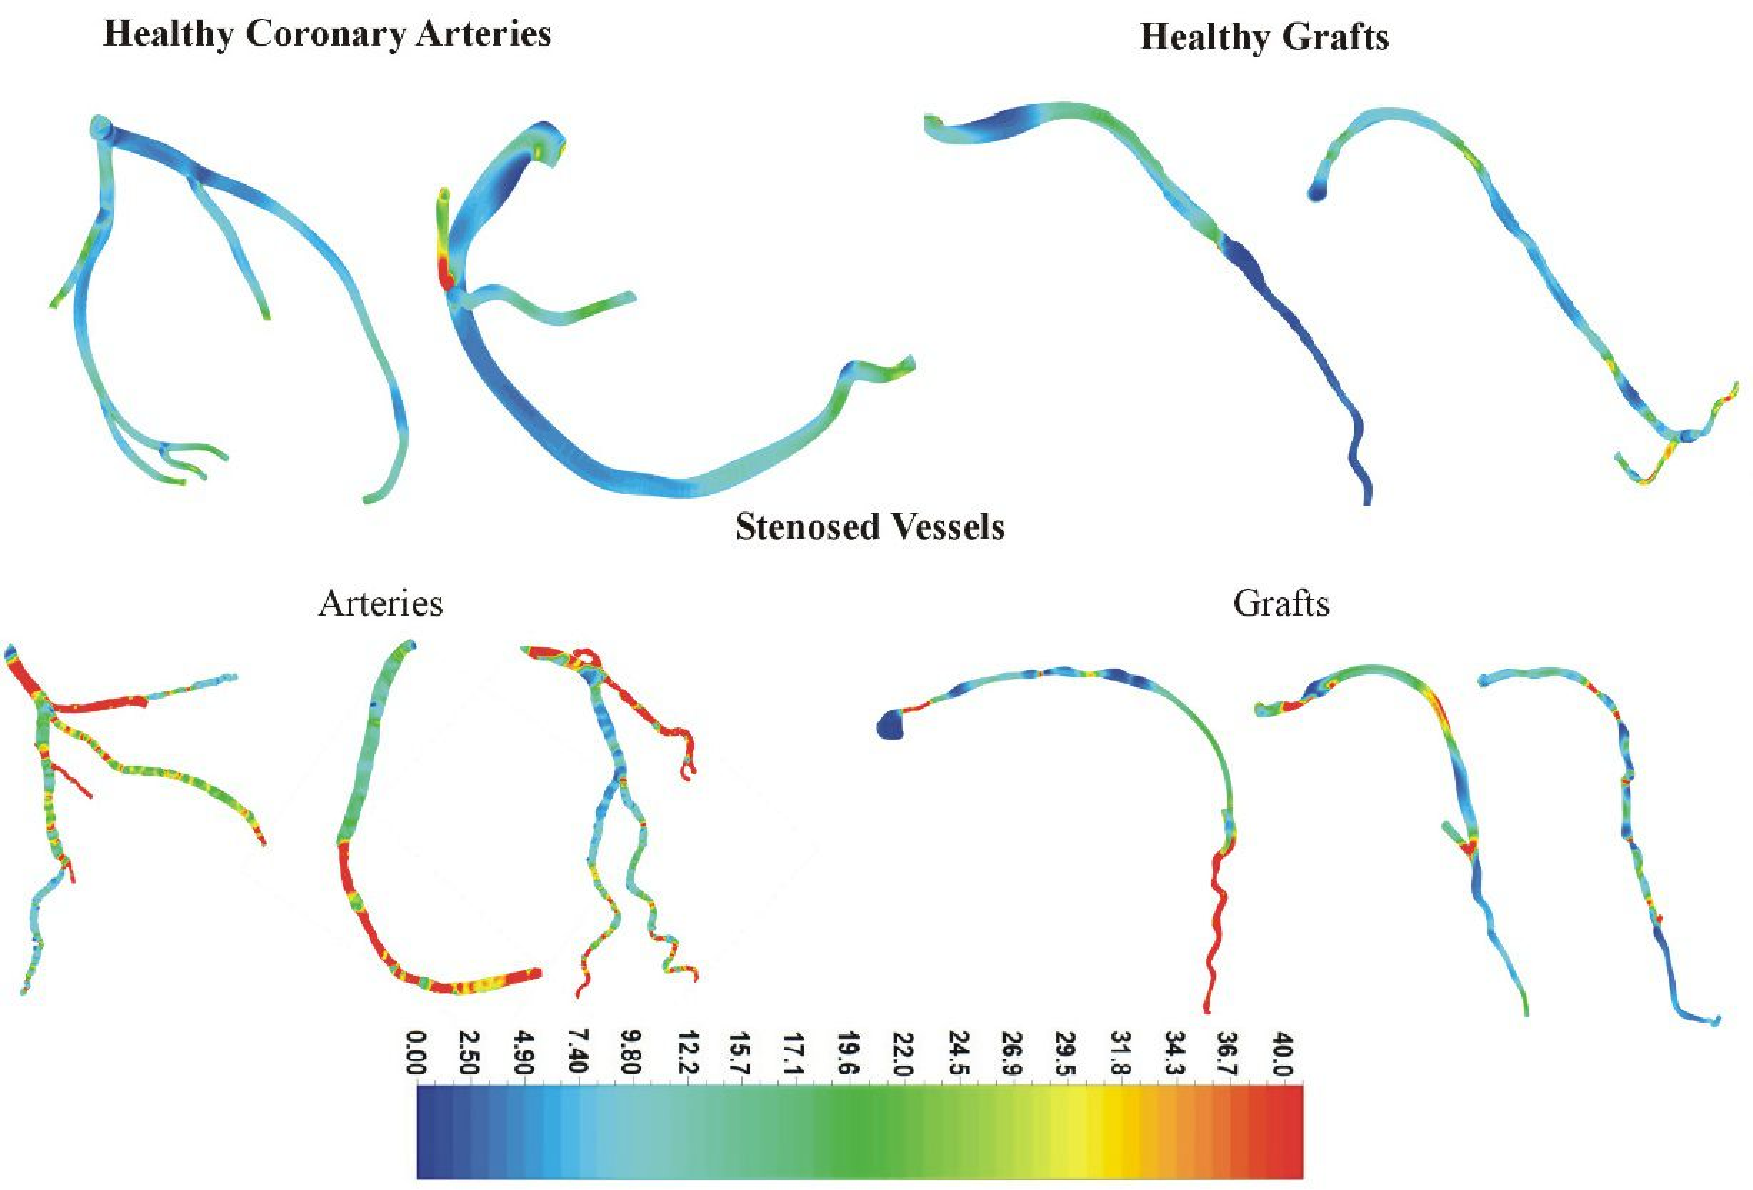
\includegraphics[width=1\textwidth]{WSS (1).pdf}
         \caption{Wall shear stress contours ( dynes/cm$^2$): (a) shows the healthy left and right coronary arteries, (b) represents the healthy grafts and (c) illustrates the stenosed grafts.}
         \label{fig:2}
     \end{figure}

\subsection{Statistical Analysis}     
The analysis is started by comparing area-weighted average WSS values along the coronary arteries between patients and controls and also between grafts with or without SVGD. We analyzed the bifurcations and the remaining portions of the arteries differently because WSS could already reach high values in bifurcations even in healthy controls and this could skew the  WSS distributions along arterial walls. The area-weighted average WSS in arterial segments outside the bifurcations was not significantly different in PCAs and DGs compared to HCAs and HGs in both Newtonian and Carreau-Yasuda models, although WSS in PCAs and DGs had a tendency to be higher for both models as illustrated in Figure \ref{fig:3}(a) for the Newtonian model and Figure \ref{fig:3}(b) for the Carreau-Yasuda model, and summarized in Table \ref{tab:b}. When bifurcations were specifically considered, WSS is found to be significantly higher in PCAs compared to HCAs, for both Newtonian and Carreau-Yasuda models as shown in Figures \ref{fig:3}(c) and \ref{fig:3}(d) and detailed in Table \ref{tab:c}. Surprisingly, HGs exhibit higher WSS at their termination points, referred to as bifurcations, compared to DGs. These points are where the grafts are surgically connected to the target area. Despite the observed differences in WSS, these variations are not statistically significant, with \textit{p}-values of 0.95 for the Newtonian model and 0.54 for the Carreau-Yasuda model. 


\begin{table}[h!]
\centering
    \setlength{\tabcolsep}{5pt}
    \renewcommand{\arraystretch}{0.9}
    \caption{Area-weighted average WSS (dynes/cm$^2$) for healthy coronary arteries, bypass grafts, and diseased coronary arteries from both datasets, analyzed using both the Newtonian and Carreau-Yasuda models.}
    \begin{tabular}{|c|c|c|c|c|c|c|c|c|c|c|c|c|c|c|c|c|c|c|c|c|c|c|c|c|c|} 
    \hline 
    \multirow{2}{*}{\textbf{Models}} & \multicolumn{4}{c|}{Healthy (H)} & \multicolumn{5}{c|}{Bypass Grafts (BG)} &\multicolumn{3}{c|}{Diseased (D)} \\ \cline{2-13} & H1 & H2 & H3 & H4 & BG1 & BG2 & BG3 & BG4 & BG5 & D1 & D2 & D3 \\ \hline
 \multicolumn{13}{|c|}{\textbf{Newtonian Model}}\\ \hline  \textbf{RCA}& 9 & 13.1 & 11.9 & 26.8& 20.6 & 5.4 & 13.8 & 48.4 & 14.8 &14.9 & 36.3 &19.7  \\ \hline  \textbf{LCA}& 9 & 13.5 & 17.8 & 12.9& - &8.7 & 24 & 11.6 & 15 & 8 &34.5& 38.5  \\ \hline 
   \textbf{Graft 1 (H)}& - & - & - & -& 9.9 & 6.8 & 14.3 & 8.5 & 13.6 & - &-& -  \\ \hline 
   \textbf{Graft 2 (H)}& - & - & - & -& 12.3 & 5.9 & 41.6 & 10.6 & 7 & - &-& - \\ \hline 
   \textbf{Graft 3 (D)}& - & - & - & -& 9.8 & 14.8 & 41.3 & 10.8 & 10.2 & - &-& - \\ \hline
  \multicolumn{13}{|c|}{\textbf{Carreau-Yasuda Model}}\\ \hline  \textbf{RCA}& 9.2 & 13.7 & 14.6 & 21.8& 32.5 & 7.6 & 14.1 & 48.5 & 15.7 &17.6 & 42.1 &29.4  \\ \hline  \textbf{LCA}& 9.2 & 14.9 & 17.4 & 14& - &9.4 & 24.4 & 12.2 & 15.5 & 12.6 &32.5& 33.3  \\ \hline 
   \textbf{Graft 1 (H)}& - & - & - & -& 10.5 & 6.9 & 14.7 & 8.9 & 14.1 & - &-& -  \\ \hline 
   \textbf{Graft 2 (H)}& - & - & - & -& 12.7 & 6.9 & 43.9 & 10.9 & 7.7 & - &-& - \\ \hline 
   \textbf{Graft 3 (D)}& - & - & - & -& 10.2 & 15.3 & 42.1 & 11.1 & 12 & - &-& - \\ \hline
   \end{tabular}
    \label{tab:b}
\end{table}

\begin{table}[h!]
\centering
    \setlength{\tabcolsep}{4.5pt}
    \renewcommand{\arraystretch}{0.9}
   \caption{Average WSS values at the bifurcations for both the RCA and LCA, as well as for the grafts, are presented. Data from both datasets are included, along with results from both the Newtonian and Carreau-Yasuda models.}
    \begin{tabular}{|c|c|c|c|c|c|c|c|c|c|c|c|c|c|c|c|c|c|c|c|c|c|c|c|c|c|} 
    \hline 
    \multirow{2}{*}{\textbf{Models}} & \multicolumn{4}{c|}{Healthy (H)} & \multicolumn{5}{c|}{Bypass Grafts (BG)} &\multicolumn{3}{c|}{Diseased (D)} \\ \cline{2-13} & H1 & H2 & H3 & H4 & BG1 & BG2 & BG3 & BG4 & BG5 & D1 & D2 & D3 \\ \hline
 \multicolumn{13}{|c|}{\textbf{Newtonian Model}}\\ \hline  \textbf{RCA}& 59.3 & 39 & 19.7 & 10.6& 69.8 & 67.3 & 30.1 & 28.7 & 51.6 &- & - &-  \\ \hline  \textbf{LCA}& 22.8 & 44.5 & 31.8 & 28.7& - &- & 87.7 & 39.3 & - & 34.7&86.9& 100.7  \\ \hline 
   \textbf{Graft 1 (H)}& - & - & - & -& 136.2 & 47.8 & 66.1 & 47.9 & 76.1 & - &-& -  \\ \hline 
   \textbf{Graft 2 (H)}& - & - & - & -& 53.1 & 1.4 & 14.1 & 10.7 & 27.7 & - &-& - \\ \hline 
   \textbf{Graft 3 (D)}& - & - & - & -& 26.1 & 15.5 & 87.7 & - & 30.1 & - &-& - \\ \hline
    \multicolumn{13}{|c|}{\textbf{Carreau-Yasuda Models}}\\ \hline  \textbf{RCA}& 57 & 33.3 & 22 & 4.1& 69.7 & 57.4 & 30.1 & 32.6 & 53.8 &- & - &-  \\ \hline  \textbf{LCA}& 20.8 & 39.5 & 28.1 & 31.3& - &- & 87.4 & 22.2 & - & 58.5& 78& 91.5  \\ \hline 
   \textbf{Graft 1 (H)}& - & - & - & -& 134.3 & 47.8 & 66.3 & 43.2 & 73.8 & - &-& -  \\ \hline 
   \textbf{Graft 2 (H)}& - & - & - & -& 52.1 & 1.4 & 15.6 & 15.7 & 28.3 & - &-& - \\ \hline 
   \textbf{Graft 3 (D)}& - & - & - & -& 25.8 & 15.5 & 61.2 & - & 31.2 & - &-& - \\ \hline
    \end{tabular}
    \label{tab:c}
\end{table}



Because we did not find a significant difference between CAD patients and healthy controls when zones outside bifurcations were analyzed for area-weighted WSS, we next tested whether certain focal zones could reach very high WSS values and whether we could identify a possible threshold that could identify CAD arteries and diseased grafts. Based on our visual observations described above, we calculated the vessel wall area fraction of arteries where WSS exceeds 40 dynes/cm$^2$. HCAs and HGs rarely exceed this threshold, while PCAs and DGs consistently show WSS values above 40 dynes/cm$^2$. This fraction is significantly larger in PCAs and DGs compared to HCAs and HGs. This is illustrated in Figure \ref{fig:3}(e) for the Newtonian model and Figure \ref{fig:3}(f) for the Carreau-Yasuda model. A summary of these findings is presented in Table \ref{tab:d}. These differences are significant for both the Newtonian and Carreau-Yasuda models.


\begin{table}[h!]
\centering
    \setlength{\tabcolsep}{6.5pt}
    \renewcommand{\arraystretch}{0.9}
    \caption{The percentage of area fraction for all vessels (healthy, diseased, and bypass grafts), under both the Newtonian and Carreau-Yasuda models.}
    \begin{tabular}{|c|c|c|c|c|c|c|c|c|c|c|c|c|c|c|c|c|c|c|c|c|c|c|c|c|c|} 
    \hline 
    \multirow{2}{*}{\textbf{Models}} & \multicolumn{4}{c|}{Healthy (H)} & \multicolumn{5}{c|}{Bypass Grafts (BG)} &\multicolumn{3}{c|}{Diseased (D)} \\ \cline{2-13} & H1 & H2 & H3 & H4 & BG1 & BG2 & BG3 & BG4 & BG5 & D1 & D2 & D3 \\ \hline
 \multicolumn{13}{|c|}{\textbf{Newtonian Model}}\\ \hline  \textbf{RCA}& 0 & 0 & 3 & 16& 32 & 3 & 5 & 44 & 5 &7 & 23 &13  \\ \hline  
 \textbf{LCA}& 0 & 0 & 10 & 6& - &6 & 25 & 7 & 1 & 1&29& 28  \\ \hline 
   \textbf{Graft 1 (H)}& - & - & - & -& 1 & 0 & 1 & 0 & 0 & - &-& -  \\ \hline 
   \textbf{Graft 2 (H)}& - & - & - & -& 0 & 0 & 57 & 0 & 2 & - &-& - \\ \hline 
   \textbf{Graft 3 (D)}& - & - & - & -& 2 & 5 & 22 & 4 & 2 & - &-& - \\ \hline
    \multicolumn{13}{|c|}{\textbf{Carreau-Yasuda Model}}\\ \hline  \textbf{RCA}& 0 & 0 & 4 & 10& 33 & 4 & 5 & 40 & 6 &6 & 26 &23  \\ \hline 
    \textbf{LCA}& 0 & 0 & 9 & 7& - &6 & 26 & 7 & 1 & 3&26& 23  \\ \hline 
   \textbf{Graft 1 (H)}& - & - & - & -& 1 & 0 & 2 & 0 & 0 & - &-& -  \\ \hline 
   \textbf{Graft 2 (H)}& - & - & - & -& 0 & 0 & 58 & 0 & 2 & - &-& - \\ \hline 
   \textbf{Graft 3 (D)}& - & - & - & -& 2 & 5 & 22 & 4 & 5 & - &-& - \\ \hline
    \end{tabular}
    \label{tab:d}
\end{table}



We then specifically analyzed the average WSS values in vessel wall zones exceeding the threshold of 40 dynes/cm$^2$. Both simulation models demonstrate statistically significant differences, for higher average WSS measurements at high-WSS zones in PCAs and DGs, compared to HCAs and HGs (Figures \ref{fig:3}(g) and \ref{fig:3}(h)). It is also important to note that the measurements for HGs closely resemble those of HCAs, while DGs exhibit measurements that are quite similar to those of PCAs, as detailed in Table \ref{tab:e}. These results indicate that arterial segments outside the bifurcation zones can heterogeneously reach to very high WSS values in diseased grafts and arteries, while overall WSS distribution outside these hot-spots are not different. We also observed that Carreau-Yasuda model was slightly better than Newtonian model to detect spots with very high WSS values above 40 dynes/cm$^2$. Carreau-Yasuda model's improved sensitivity suggests that it better captures the nuances of non-Newtonian blood behavior, particularly in diseased vessels.

\begin{table}[h!]
\centering
    \setlength{\tabcolsep}{5pt}
    \renewcommand{\arraystretch}{0.9}
    \caption{The area-weighted average WSS for vessel areas that exceed the threshold value of 40 dynes/cm$^2$ for both healthy and diseased vessels under both Newtonian and Carreau-Yasuda models.}    \begin{tabular}{|c|c|c|c|c|c|c|c|c|c|c|c|c|c|c|c|c|c|c|c|c|c|c|c|c|c|} 
    \hline 
    \multirow{2}{*}{\textbf{Models}} & \multicolumn{4}{c|}{Healthy (H)} & \multicolumn{5}{c|}{Bypass Grafts (BG)} &\multicolumn{3}{c|}{Diseased (D)} \\ \cline{2-13}& H1 & H2 & H3 & H4 & BG1 & BG2 & BG3 & BG4 & BG5 & D1 & D2 & D3 \\ \hline
 \multicolumn{13}{|c|}{\textbf{Newtonian Model}}\\ \hline  \textbf{RCA}& 0 & 0 & 47.7 & 52.5& 49.9 & 62.2 & 54.9 & 95.0 & 44.7 &54.5 & 98.7 &61.5  \\ \hline  \textbf{LCA}& 0 & 0 & 51.7 & 50.6& - &51.2 & 61.1 & 55.6 & 44 & 48.5 &83.7& 83.2  \\ \hline 
   \textbf{Graft 1 (H)}& - & - & - & -& 53.3 & 0 & 42.8 & 0 & 0 & - &-& -  \\ \hline 
   \textbf{Graft 2 (H)}& - & - & - & -& 0 & 0 & 62.7 & 0 & 54 & - &-& - \\ \hline 
   \textbf{Graft 3 (D)}& - & - & - & -& 62.2 & 57.2 & 147.8 & 52.7 & 44.6 & - &-& - \\ \hline
 \multicolumn{13}{|c|}{\textbf{Carreau-Yasuda Model}}\\ \hline  \textbf{RCA}& 0 & 0 & 47.9 & 47.5& 67.2 & 56.8 & 54.7 & 95.6 & 47 &53.6 & 106.1 &59.3  \\ \hline  
 \textbf{LCA}& 0 & 0 & 52.3 & 50.7& - &51.6 & 61.3 & 55.5 & 44 & 47.5 &80.8& 78.4  \\ \hline 
   \textbf{Graft 1 (H)}& - & - & - & -& 43.2 & 0 & 42.9 & 0 & 0 & - &-& -  \\ \hline 
   \textbf{Graft 2 (H)}& - & - & - & -& 0 & 0 & 63.7 & 0 & 54.8 & - &-& - \\ \hline 
   \textbf{Graft 3 (D)}& - & - & - & -& 61.5 & 58.4 & 146.4 & 52.9 & 53.3 & - &-& - \\ \hline
    \end{tabular}
    \label{tab:e}
\end{table}



In line with the above results, IQR of WSS, as depicted in Figures \ref{fig:3}(i) and \ref{fig:3}(j), as well as summarized in Table \ref{tab:f}, is notably higher in PCAs than HCAs. This indicates greater variability in WSS within diseased vessels, reflecting disturbed flow patterns and fluctuating shear stress that contribute to endothelial dysfunction. This difference is only statistically significant for the Carreau-Yasuda model. This finding indicates a higher variability in WSS within diseased vessels, resulting in localized areas of both high and low shear stress, which can lead to plaque instability and vascular remodeling. In fact, it has been previously suggested that in changes in WSS gradients, and sharp changes in WSS along the vascular path can be a determinant of atherosclerotic vascular changes \cite{72, 73}. On the other hand, we did not detect significant difference between HGs and DGs for both Newtonian and Carreau-Yasuda models. 

\begin{table}[h!]
\centering
    \setlength{\tabcolsep}{5pt}
    \renewcommand{\arraystretch}{0.9}
    \caption{Interquartile Range (IQR) of WSS Values for healthy coronary arteries, bypass grafts, and diseased coronary arteries as determined by both the Newtonian and Carreau-Yasuda models. The IQR serves as a measure of statistical dispersion, highlighting the variability of WSS within each vessel category.}
    \begin{tabular}{|c|c|c|c|c|c|c|c|c|c|c|c|c|c|c|c|c|c|c|c|c|c|c|c|c|c|} 
    \hline 
    \multirow{2}{*}{\textbf{Models}} & \multicolumn{4}{c|}{Healthy (H)} & \multicolumn{5}{c|}{Bypass Grafts (BG)} &\multicolumn{3}{c|}{Diseased (D)} \\ \cline{2-13}& H1 & H2 & H3 & H4 & BG1 & BG2 & BG3 & BG4 & BG5 & D1 & D2 & D3 \\ \hline
    \multicolumn{13}{|c|}{\textbf{Newtonian Model}}\\ \hline  \textbf{RCA}& 7.3 & 12.6 & 7.3 & 19.6& 47.2 & 3.6 & 16.2 & 89.2 & 18.2 &13.2 & 24.1 &19.4  \\ \hline  \textbf{LCA}& 5.8 & 12 & 20.9 & 10.8& - &8.8 & 39.5 & 9.3 & 15.7 & 6.5 &36.3& 31.8  \\ \hline 
   \textbf{Graft 1 (H)}& - & - & - & -& 6.3 & 3.8 & 11.9 & 7 & 6.4 & - &-& -  \\ \hline 
   \textbf{Graft 2 (H)}& - & - & - & -& 10.1 & 9.6 & 46.4 & 7.2 & 5.4 & - &-& - \\ \hline 
   \textbf{Graft 3 (D)}& - & - & - & -& 8 & 13.1 & 30.1 & 8.4 & 8.2 & - &-& - \\ \hline
    \multicolumn{13}{|c|}{\textbf{Carreau-Yasuda Model}}\\ \hline  \textbf{RCA}& 6.9 & 13.7 & 7.6 & 15.3& 46.9& 6.6 & 16.6 & 88.6 & 19 &13.9 & 27.7 &24.8  \\ \hline  \textbf{LCA}& 5.4 & 11.3 & 18.4 & 11.2& - &9 & 40.9 & 9.1 & 16.7 & 10 &32.3& 24.4  \\ \hline 
   \textbf{Graft 1 (H)}& - & - & - & -& 6.2 & 3.7 & 11.2 & 7 & 6.2 & - &-& -  \\ \hline 
   \textbf{Graft 2 (H)}& - & - & - & -& 9.5 & 9.1 & 41 & 6.6 & 5.4 & - &-& - \\ \hline 
   \textbf{Graft 3 (D)}& - & - & - & -& 7.9 & 9.4 & 30.5 & 8.6 & 8.2 & - &-& - \\ \hline
    \end{tabular}
    \label{tab:f}
\end{table}



% (removed stray \setcounter{figure}{4} so figures number continuously 1--11)

\begin{figure}[h!]
    \hspace{-2cm}
    \centering
    \begin{subfigure}[b]{0.5\textwidth}
        \centering
        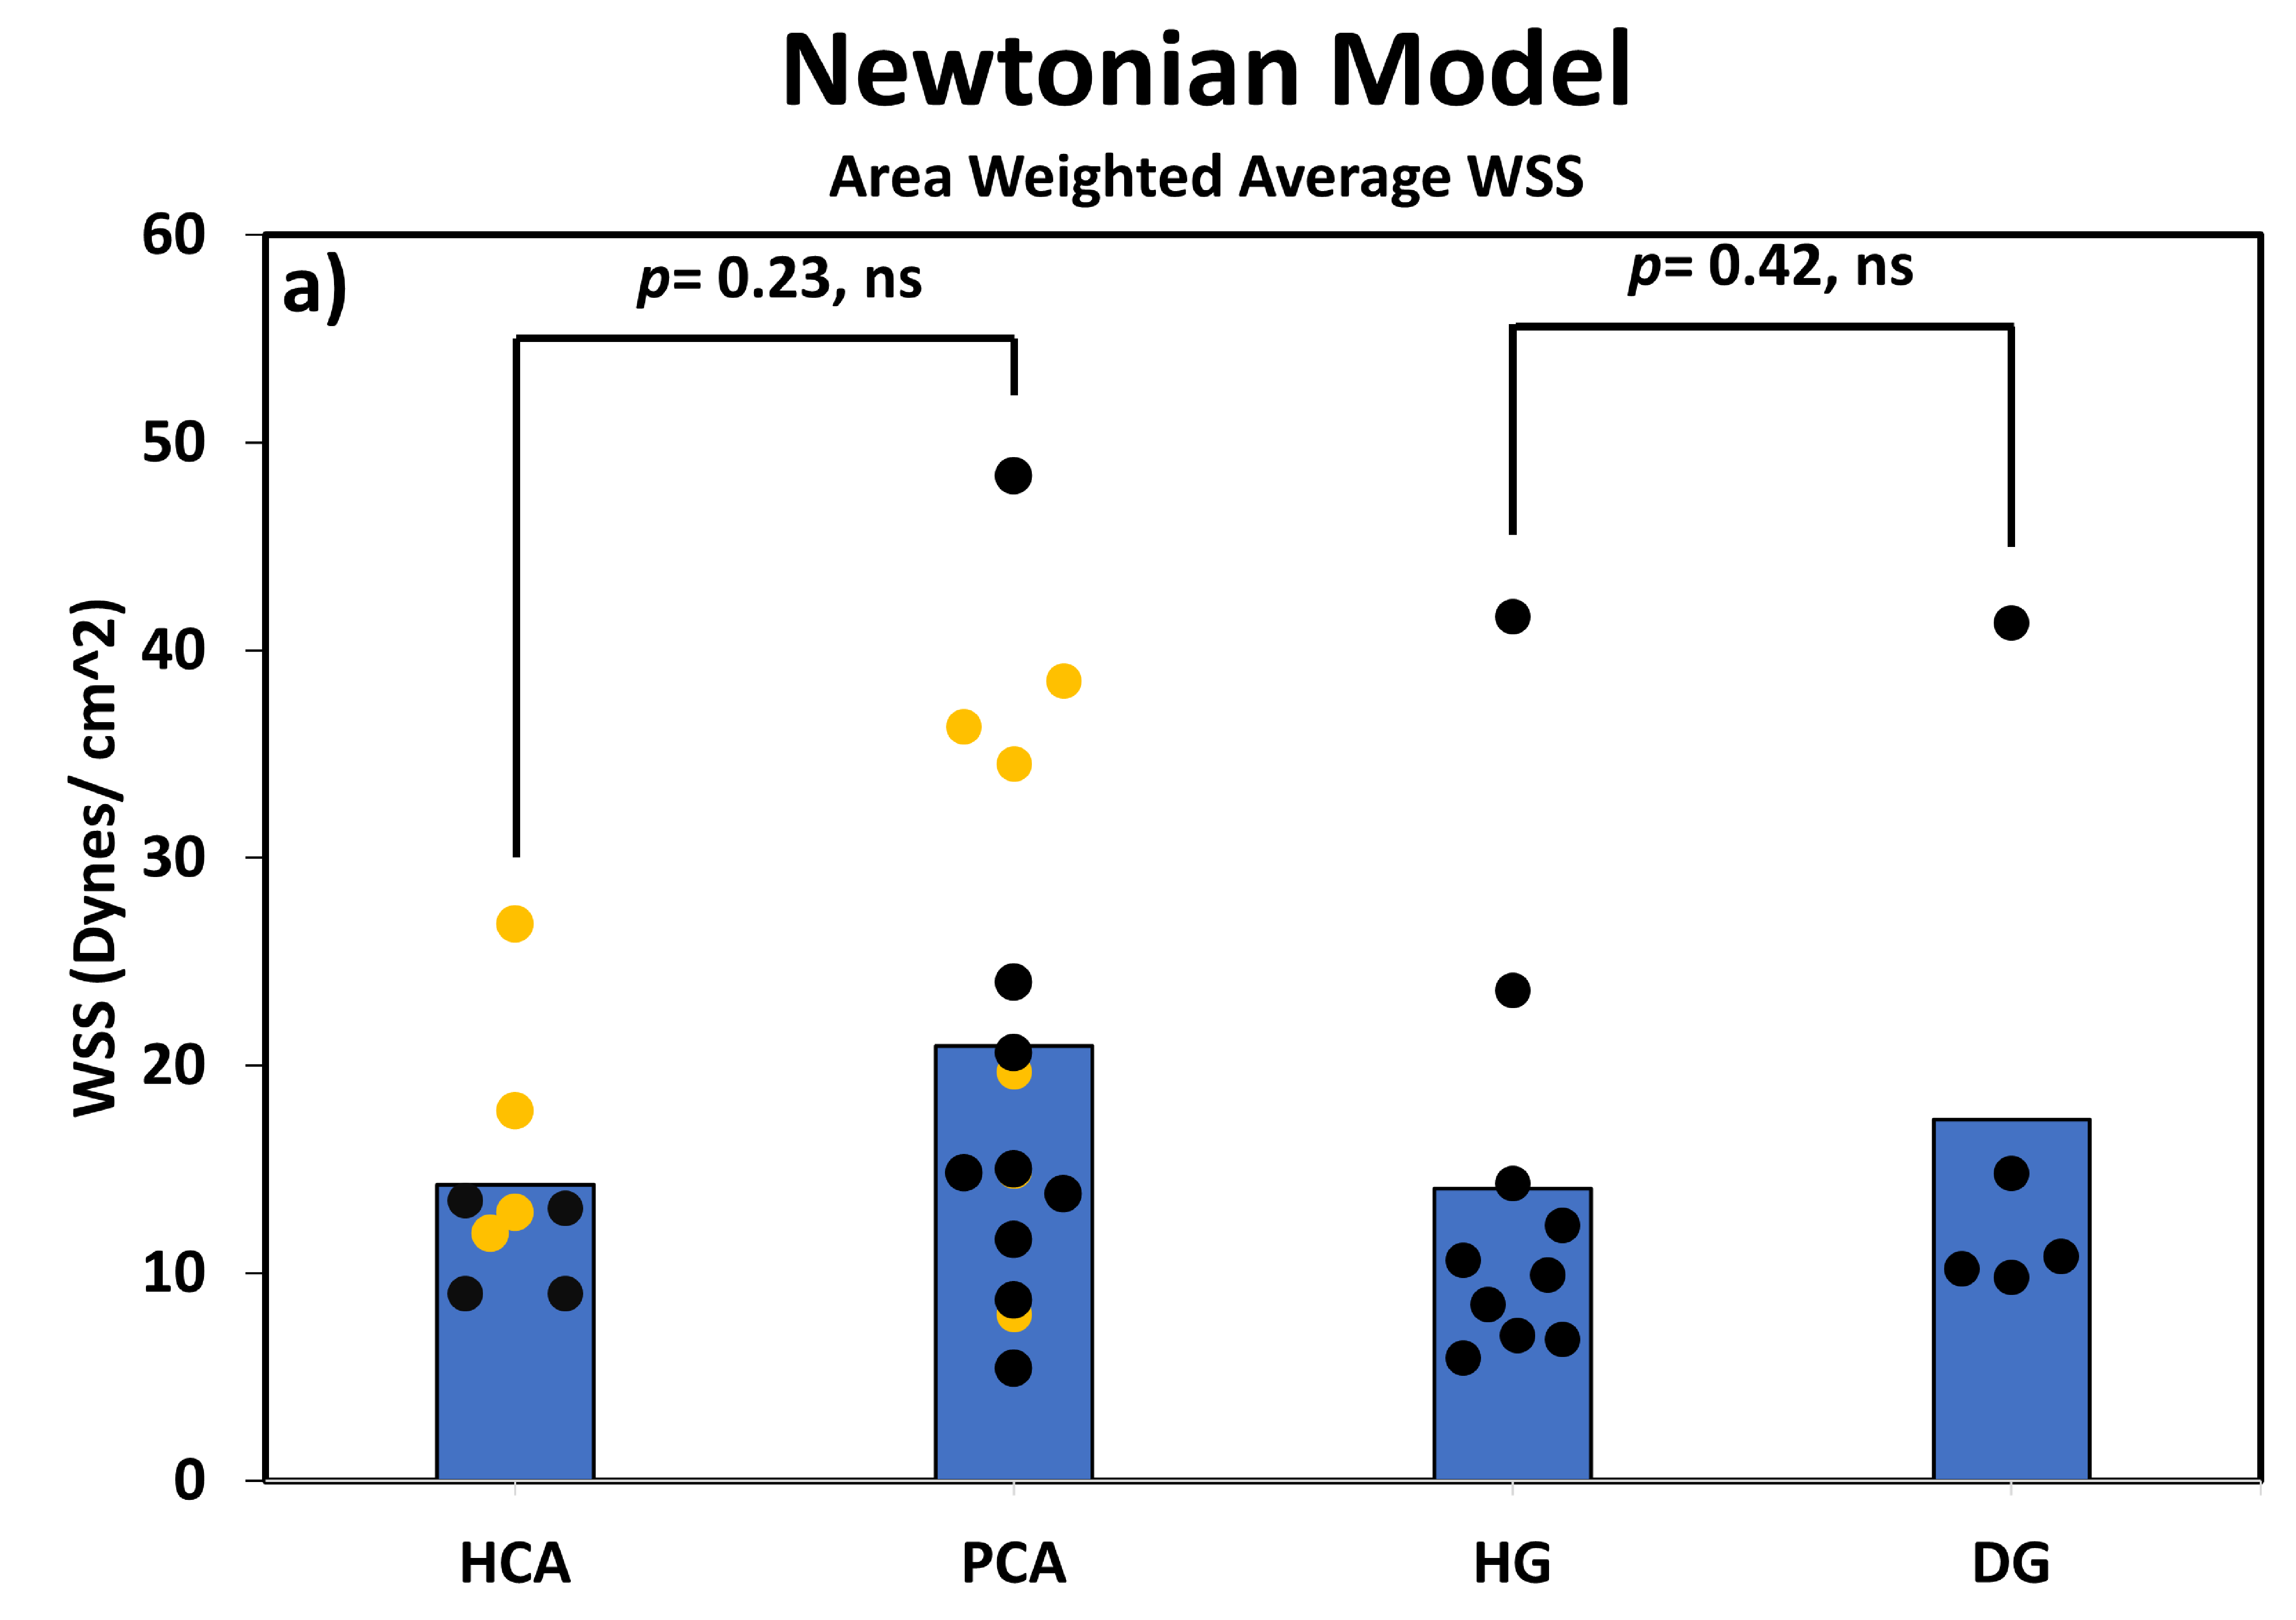
\includegraphics[width=9cm,height=7cm]{Newtonian AWAWSS (2) (1).pdf}
    \end{subfigure}
    \hspace{1cm}
    \begin{subfigure}[b]{0.5\textwidth}
        \centering
        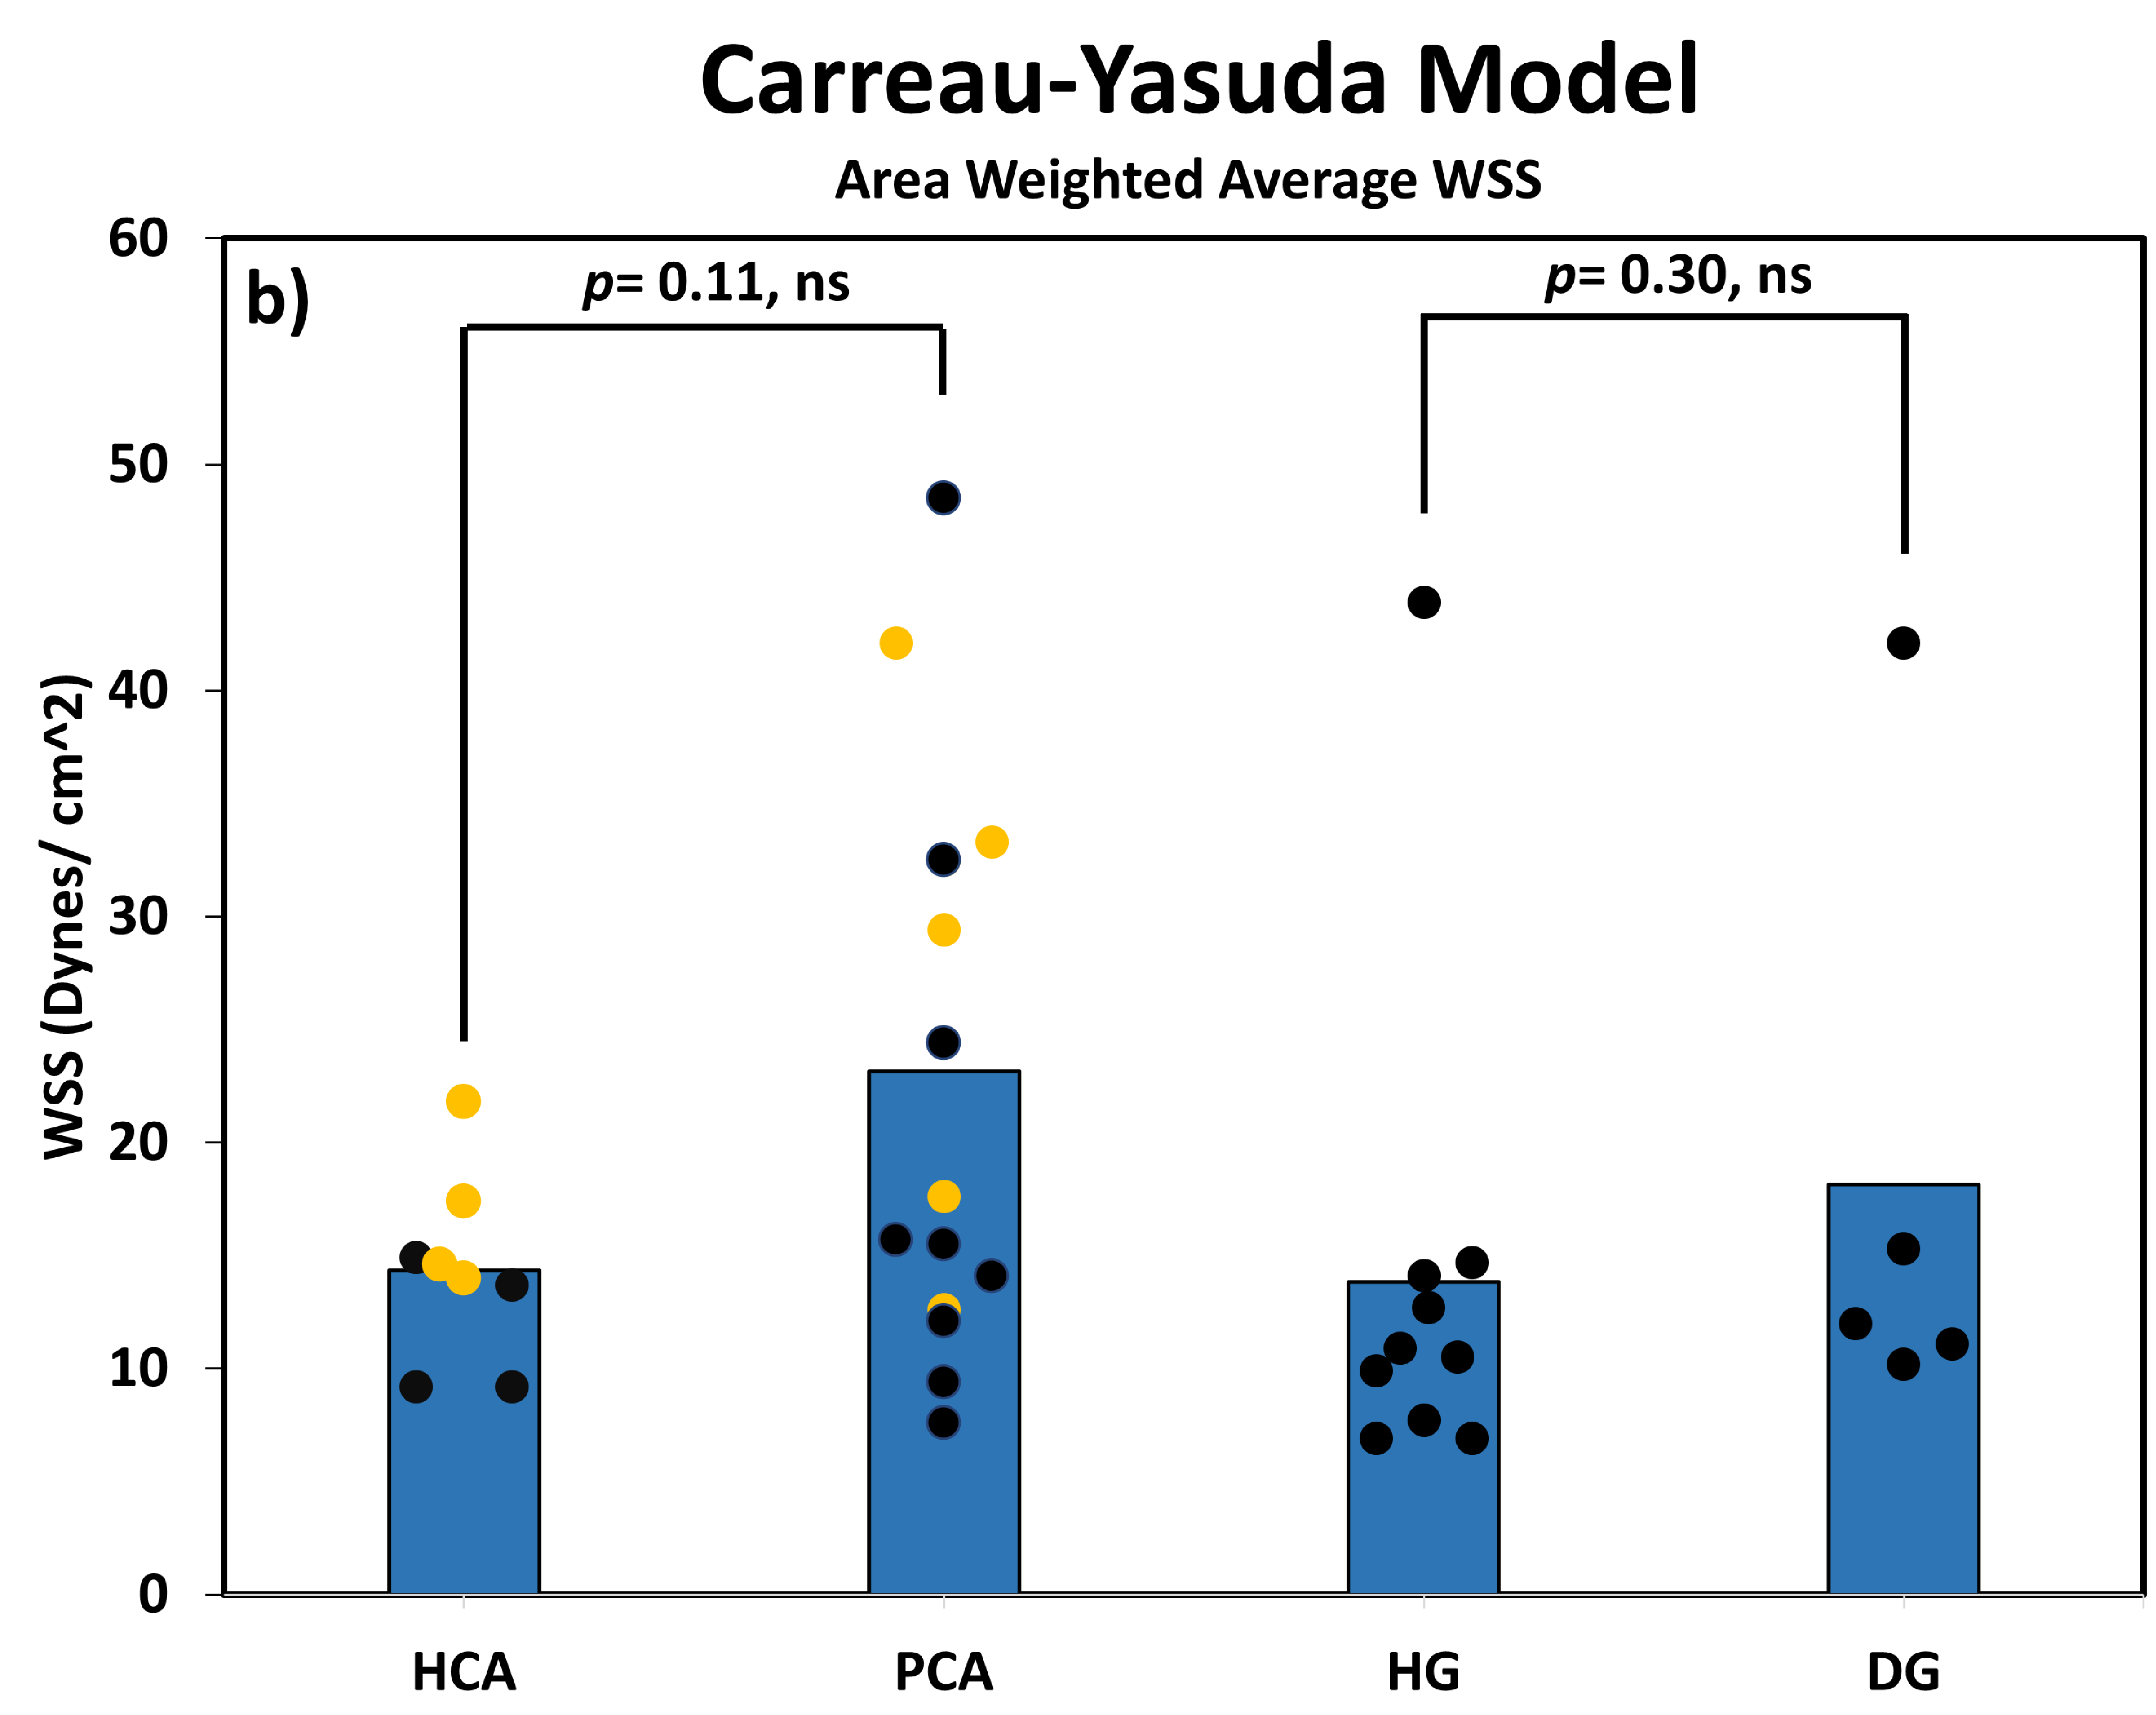
\includegraphics[width=9cm,height=7cm]{Carreau AWAWSS (2) (1).pdf}
    \end{subfigure}
    \\
    \hspace{-2cm}
    \centering
    \begin{subfigure}[c]{0.5\textwidth}
        \centering
        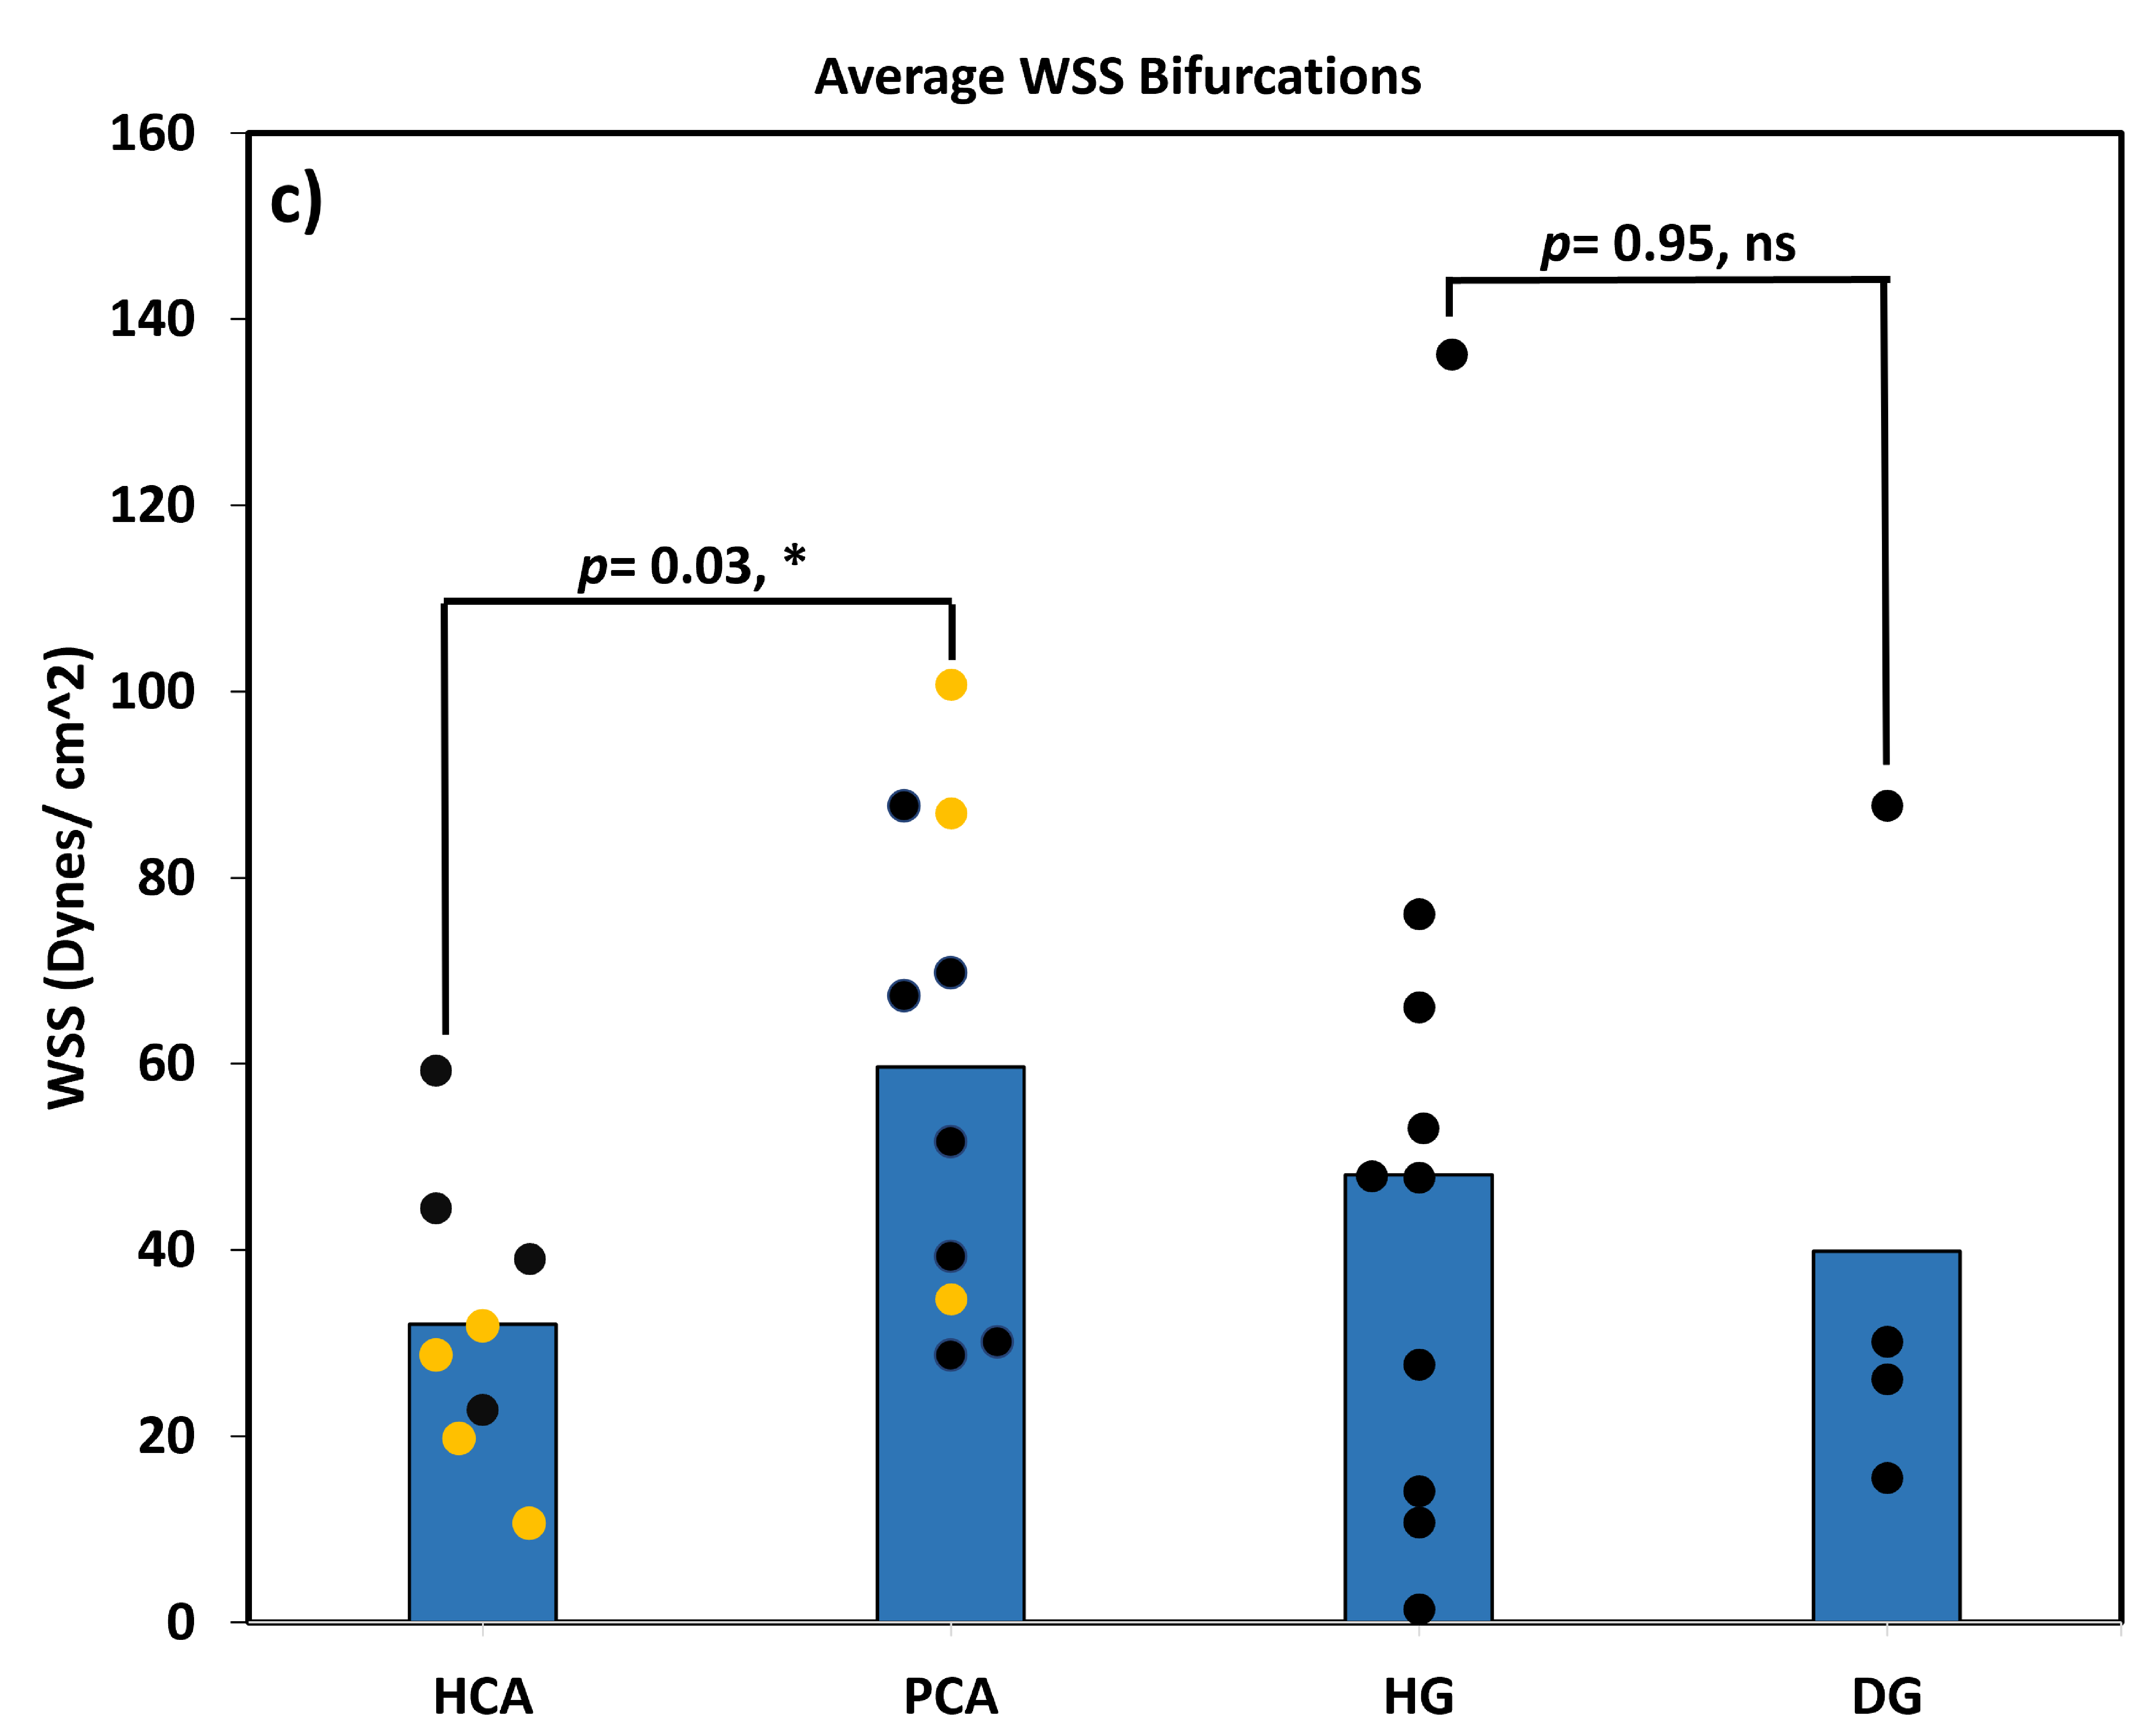
\includegraphics[width=9cm,height=7cm]{WSS Bifurcaions Newtonain (1) (1).pdf}
    \end{subfigure}
    \hspace{1cm}
    \begin{subfigure}[d]{0.5\textwidth}
        \centering
        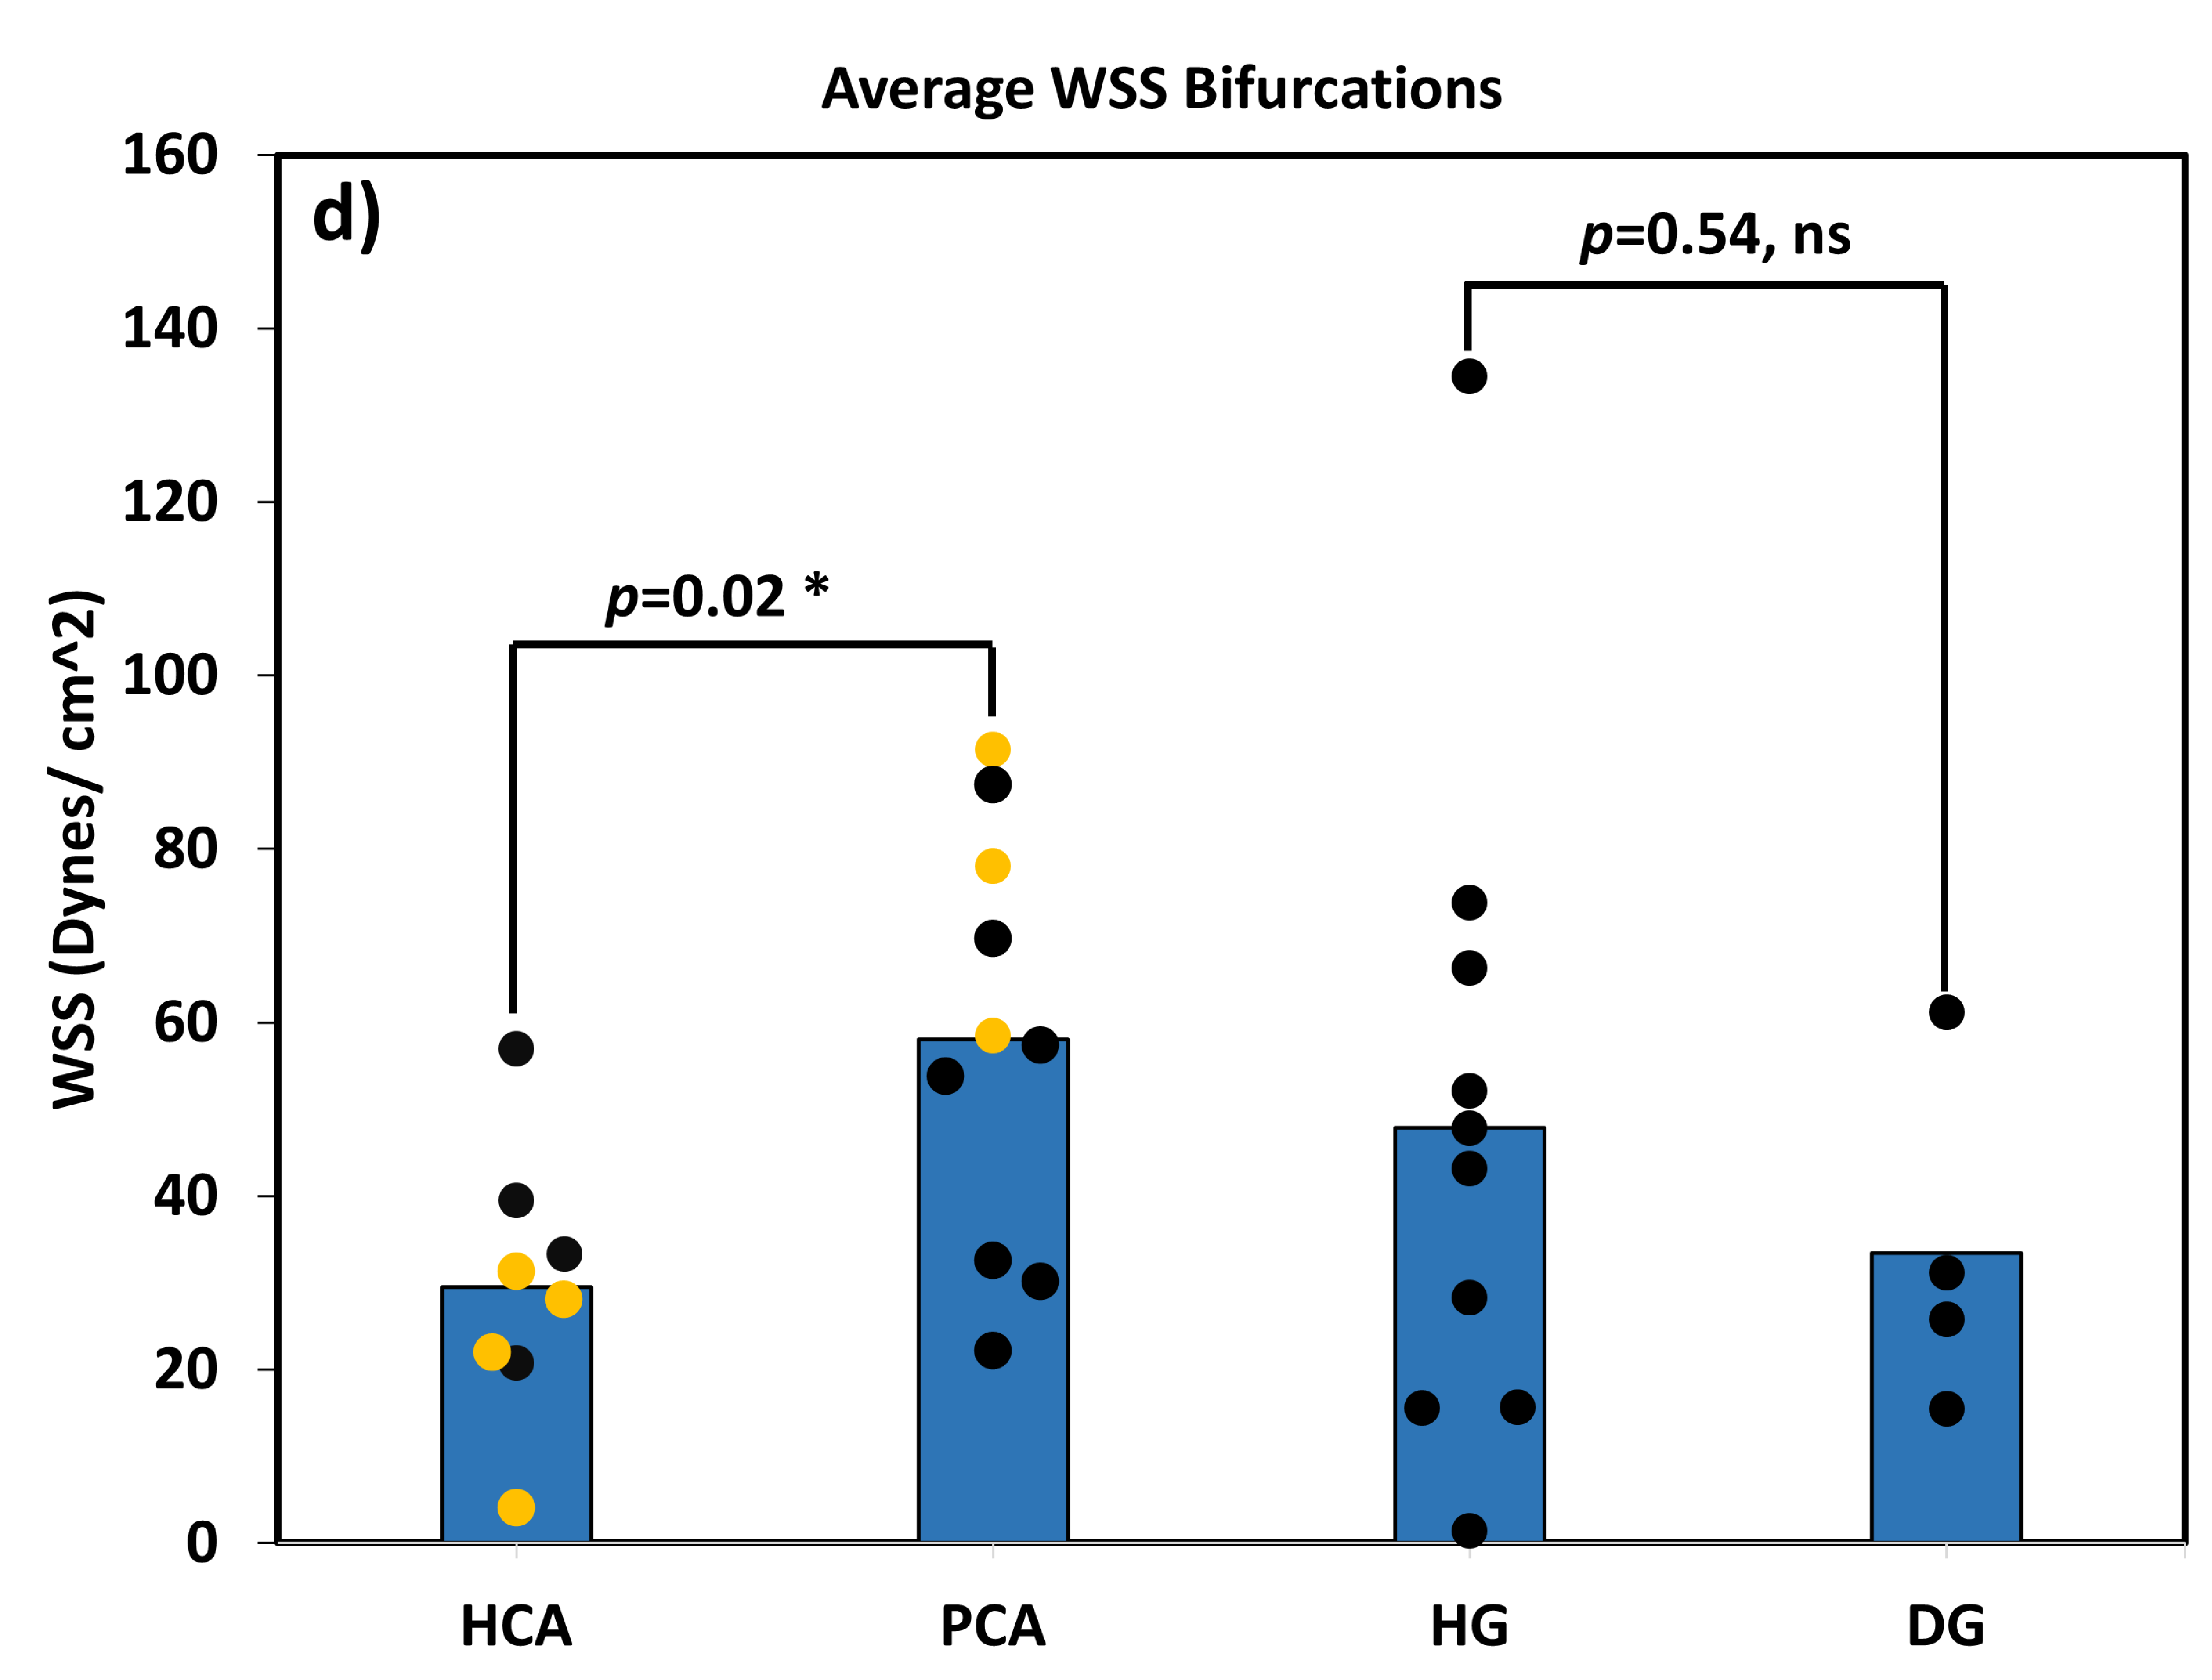
\includegraphics[width=9cm,height=7cm]{Carreau WSS Bifurcations (1) (1).pdf}
    \end{subfigure}
    \\
   \hspace{-2cm}
    \centering
    \begin{subfigure}[c]{0.5\textwidth}
        \centering
        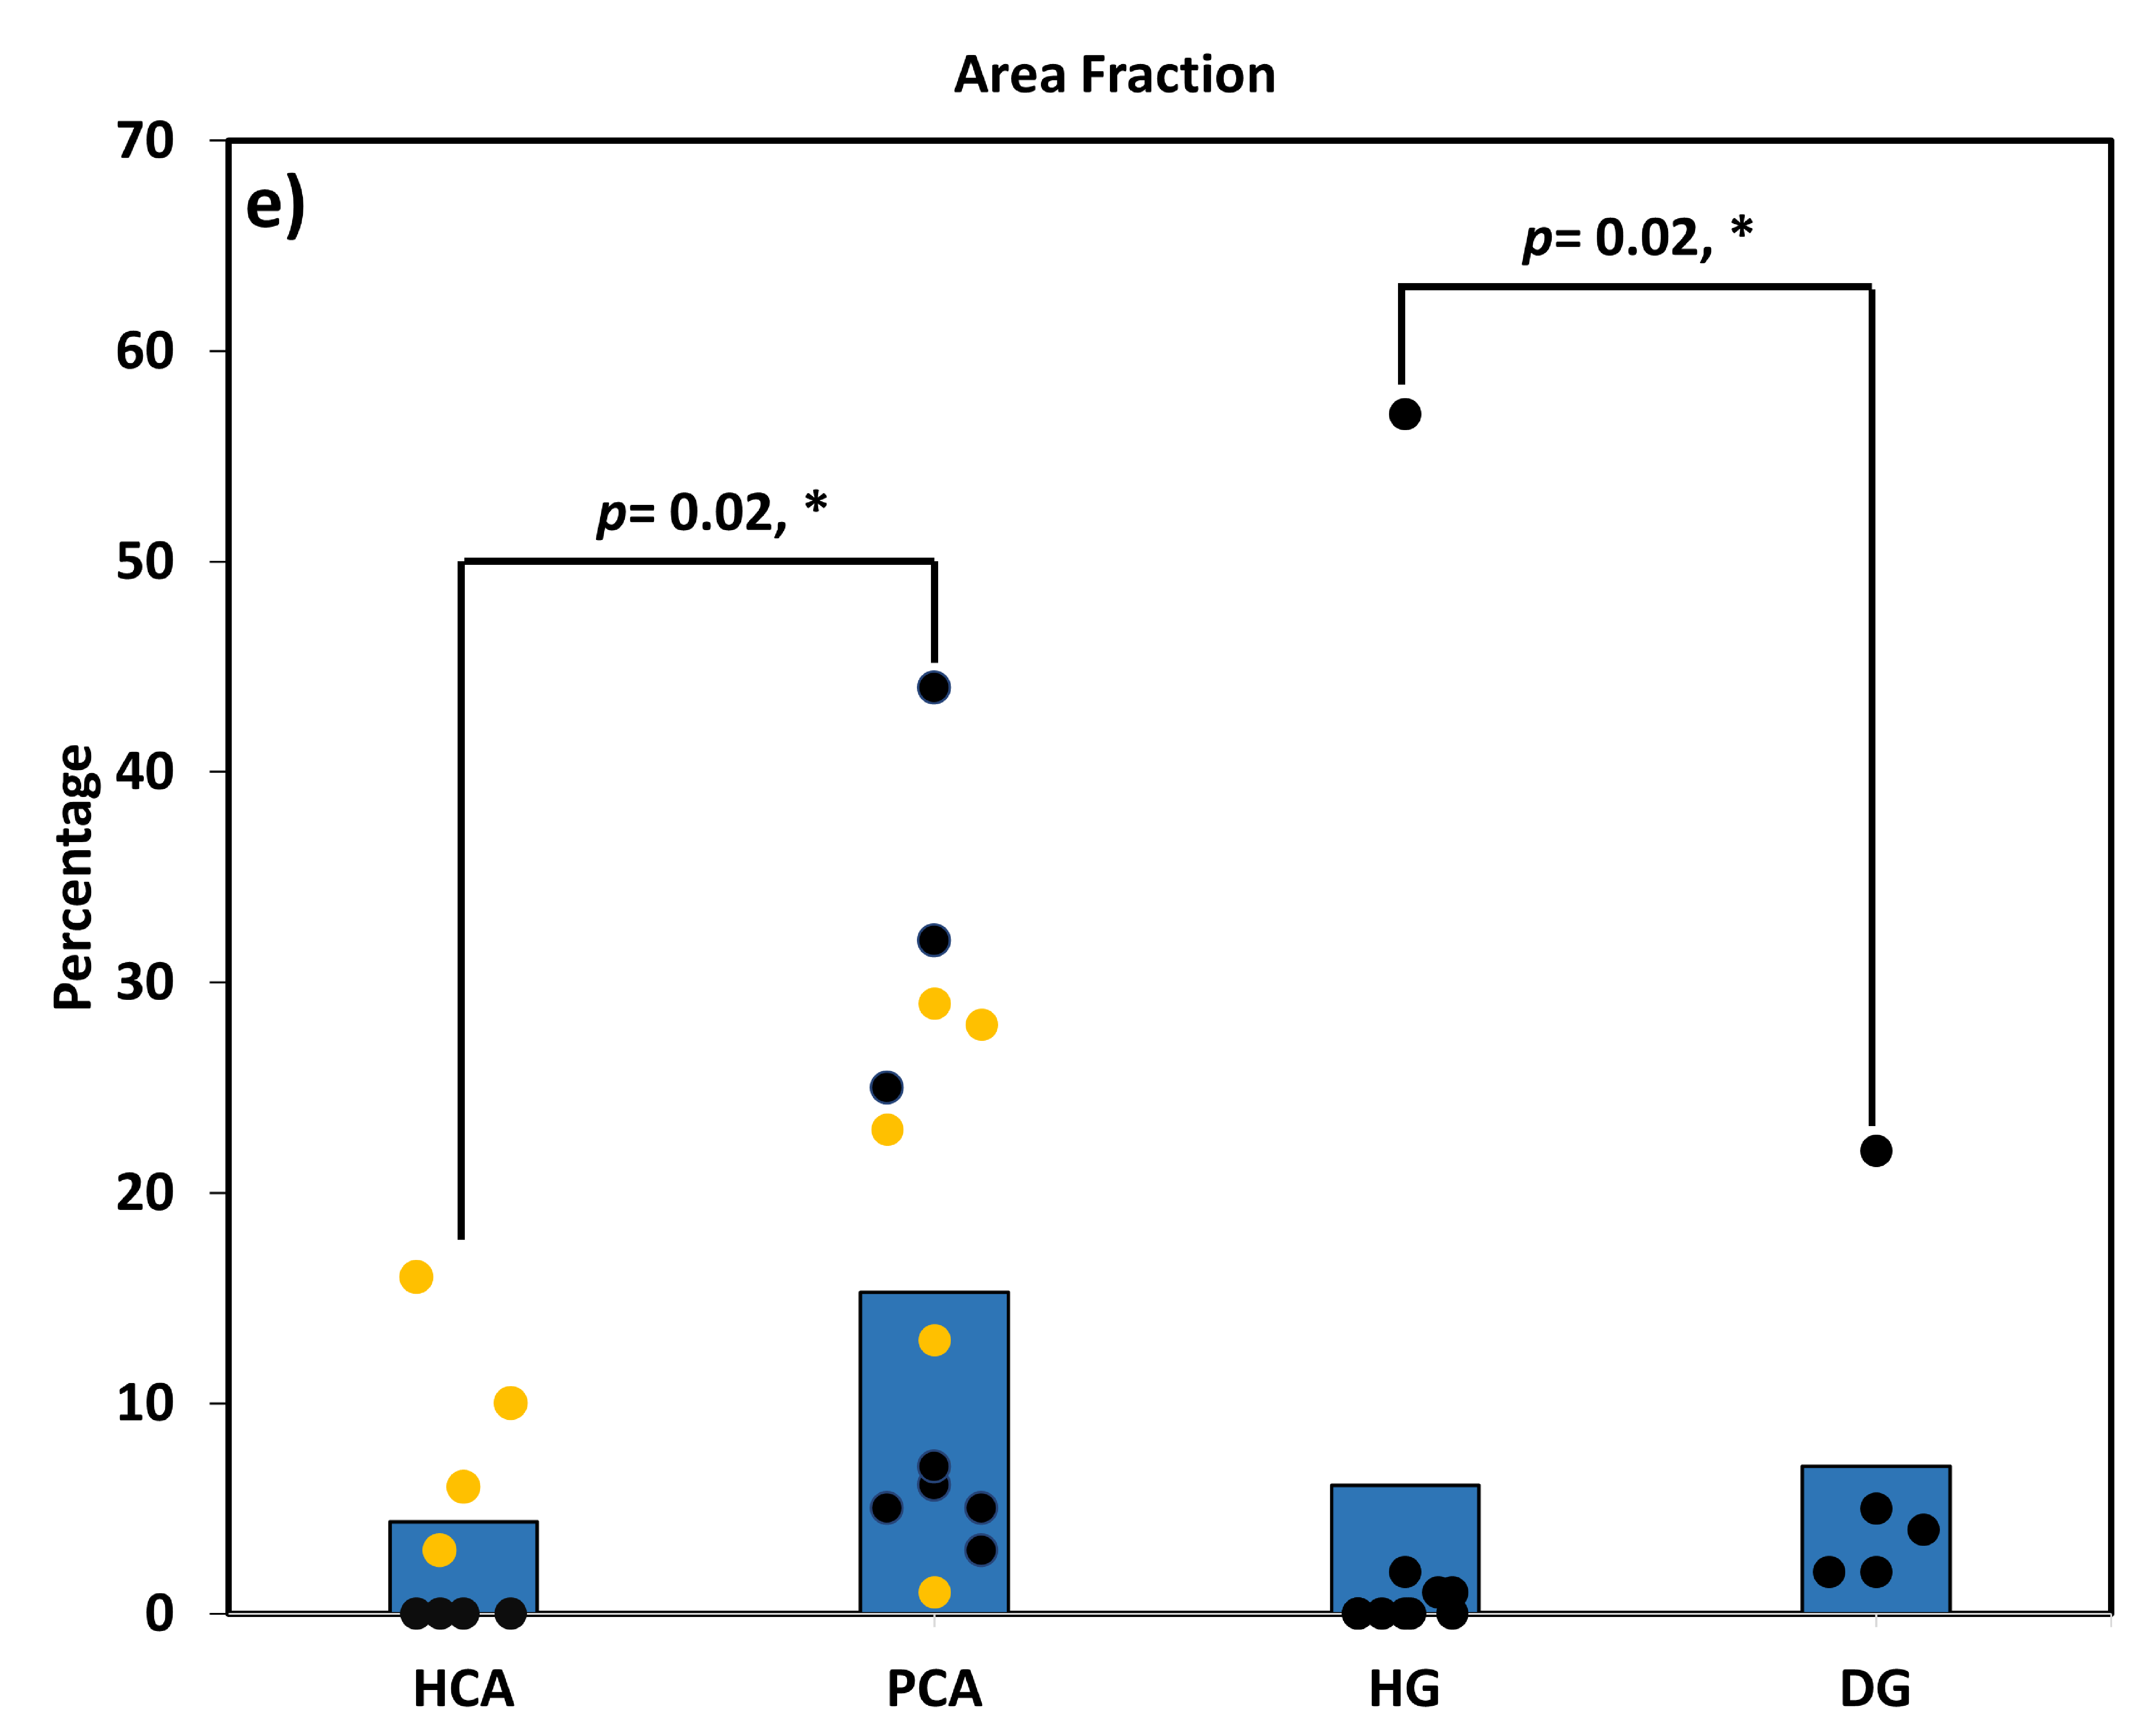
\includegraphics[width=9cm,height=7cm]{Area Fraction Newtonian (1) (1).pdf}
    \end{subfigure}
    \hspace{1cm}
    \begin{subfigure}[d]{0.5\textwidth}
        \centering
        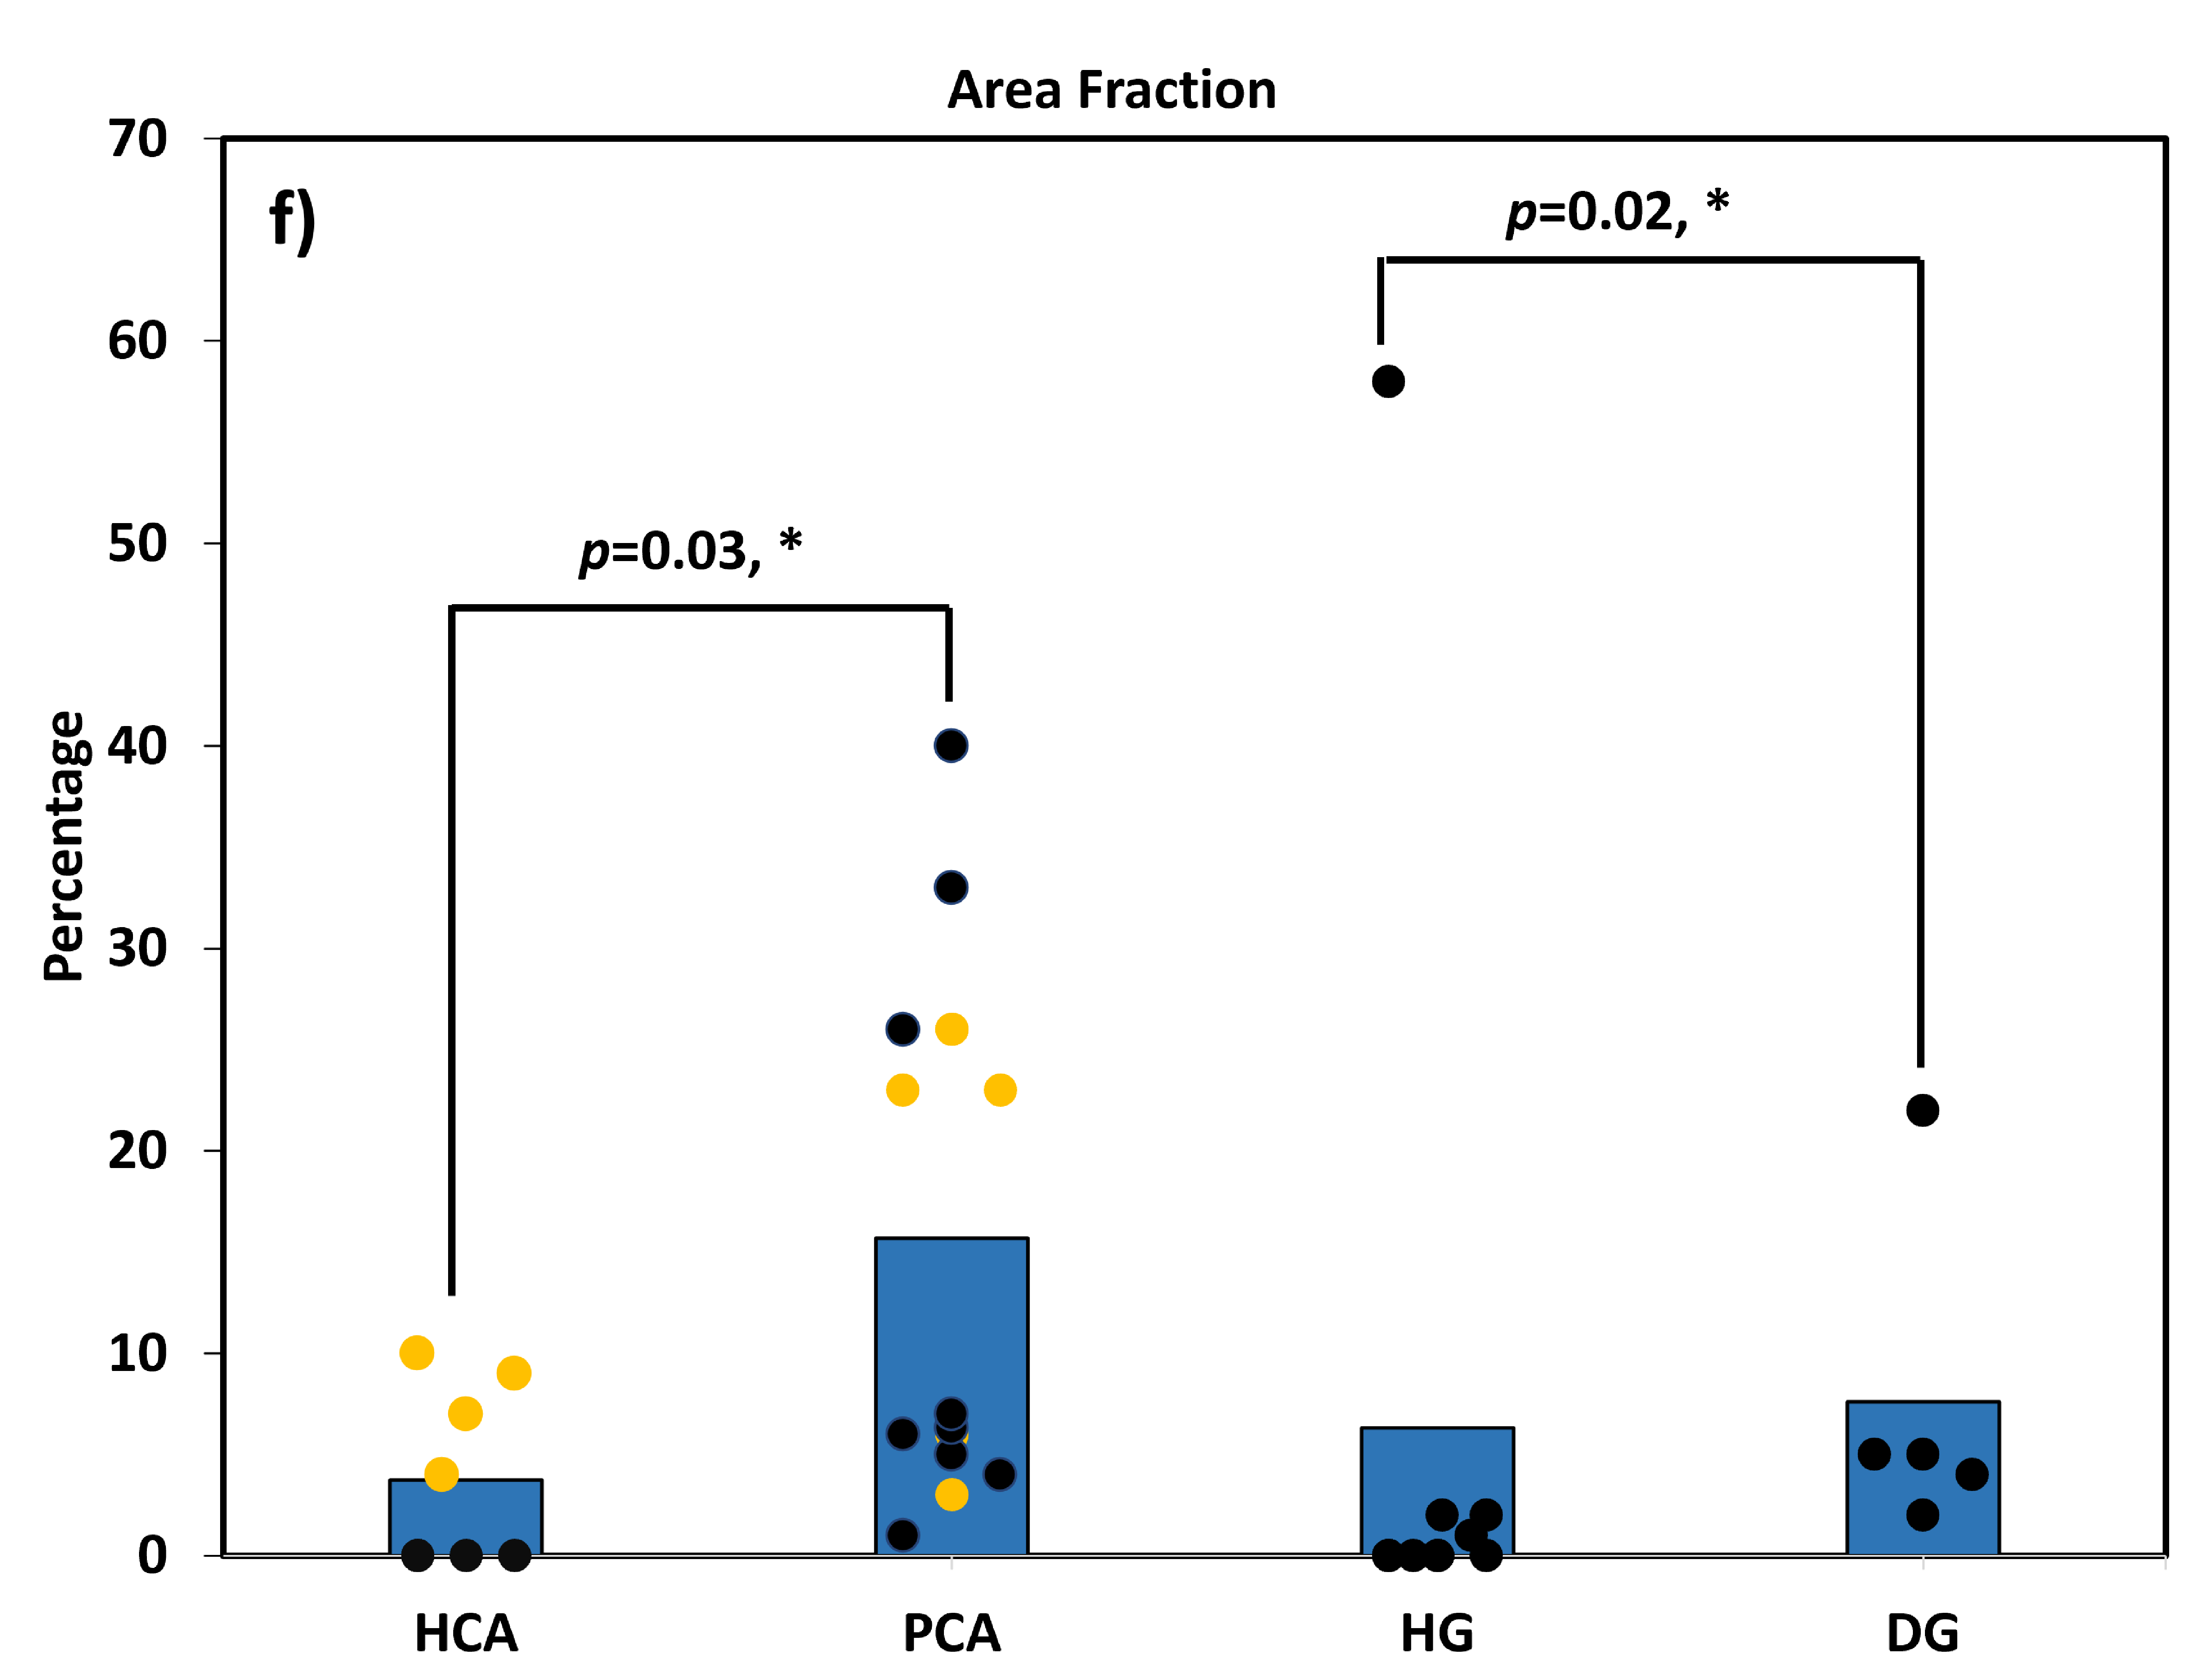
\includegraphics[width=9cm,height=7cm]{Carreau Area Fraction (1) (1).pdf}
    \end{subfigure}
\end{figure}

% Start the second page for the figures and continue the caption
\begin{figure}[h!]
    \ContinuedFloat
    \hspace{-2cm}
    \centering
    \begin{subfigure}[c]{0.5\textwidth}
        \centering
        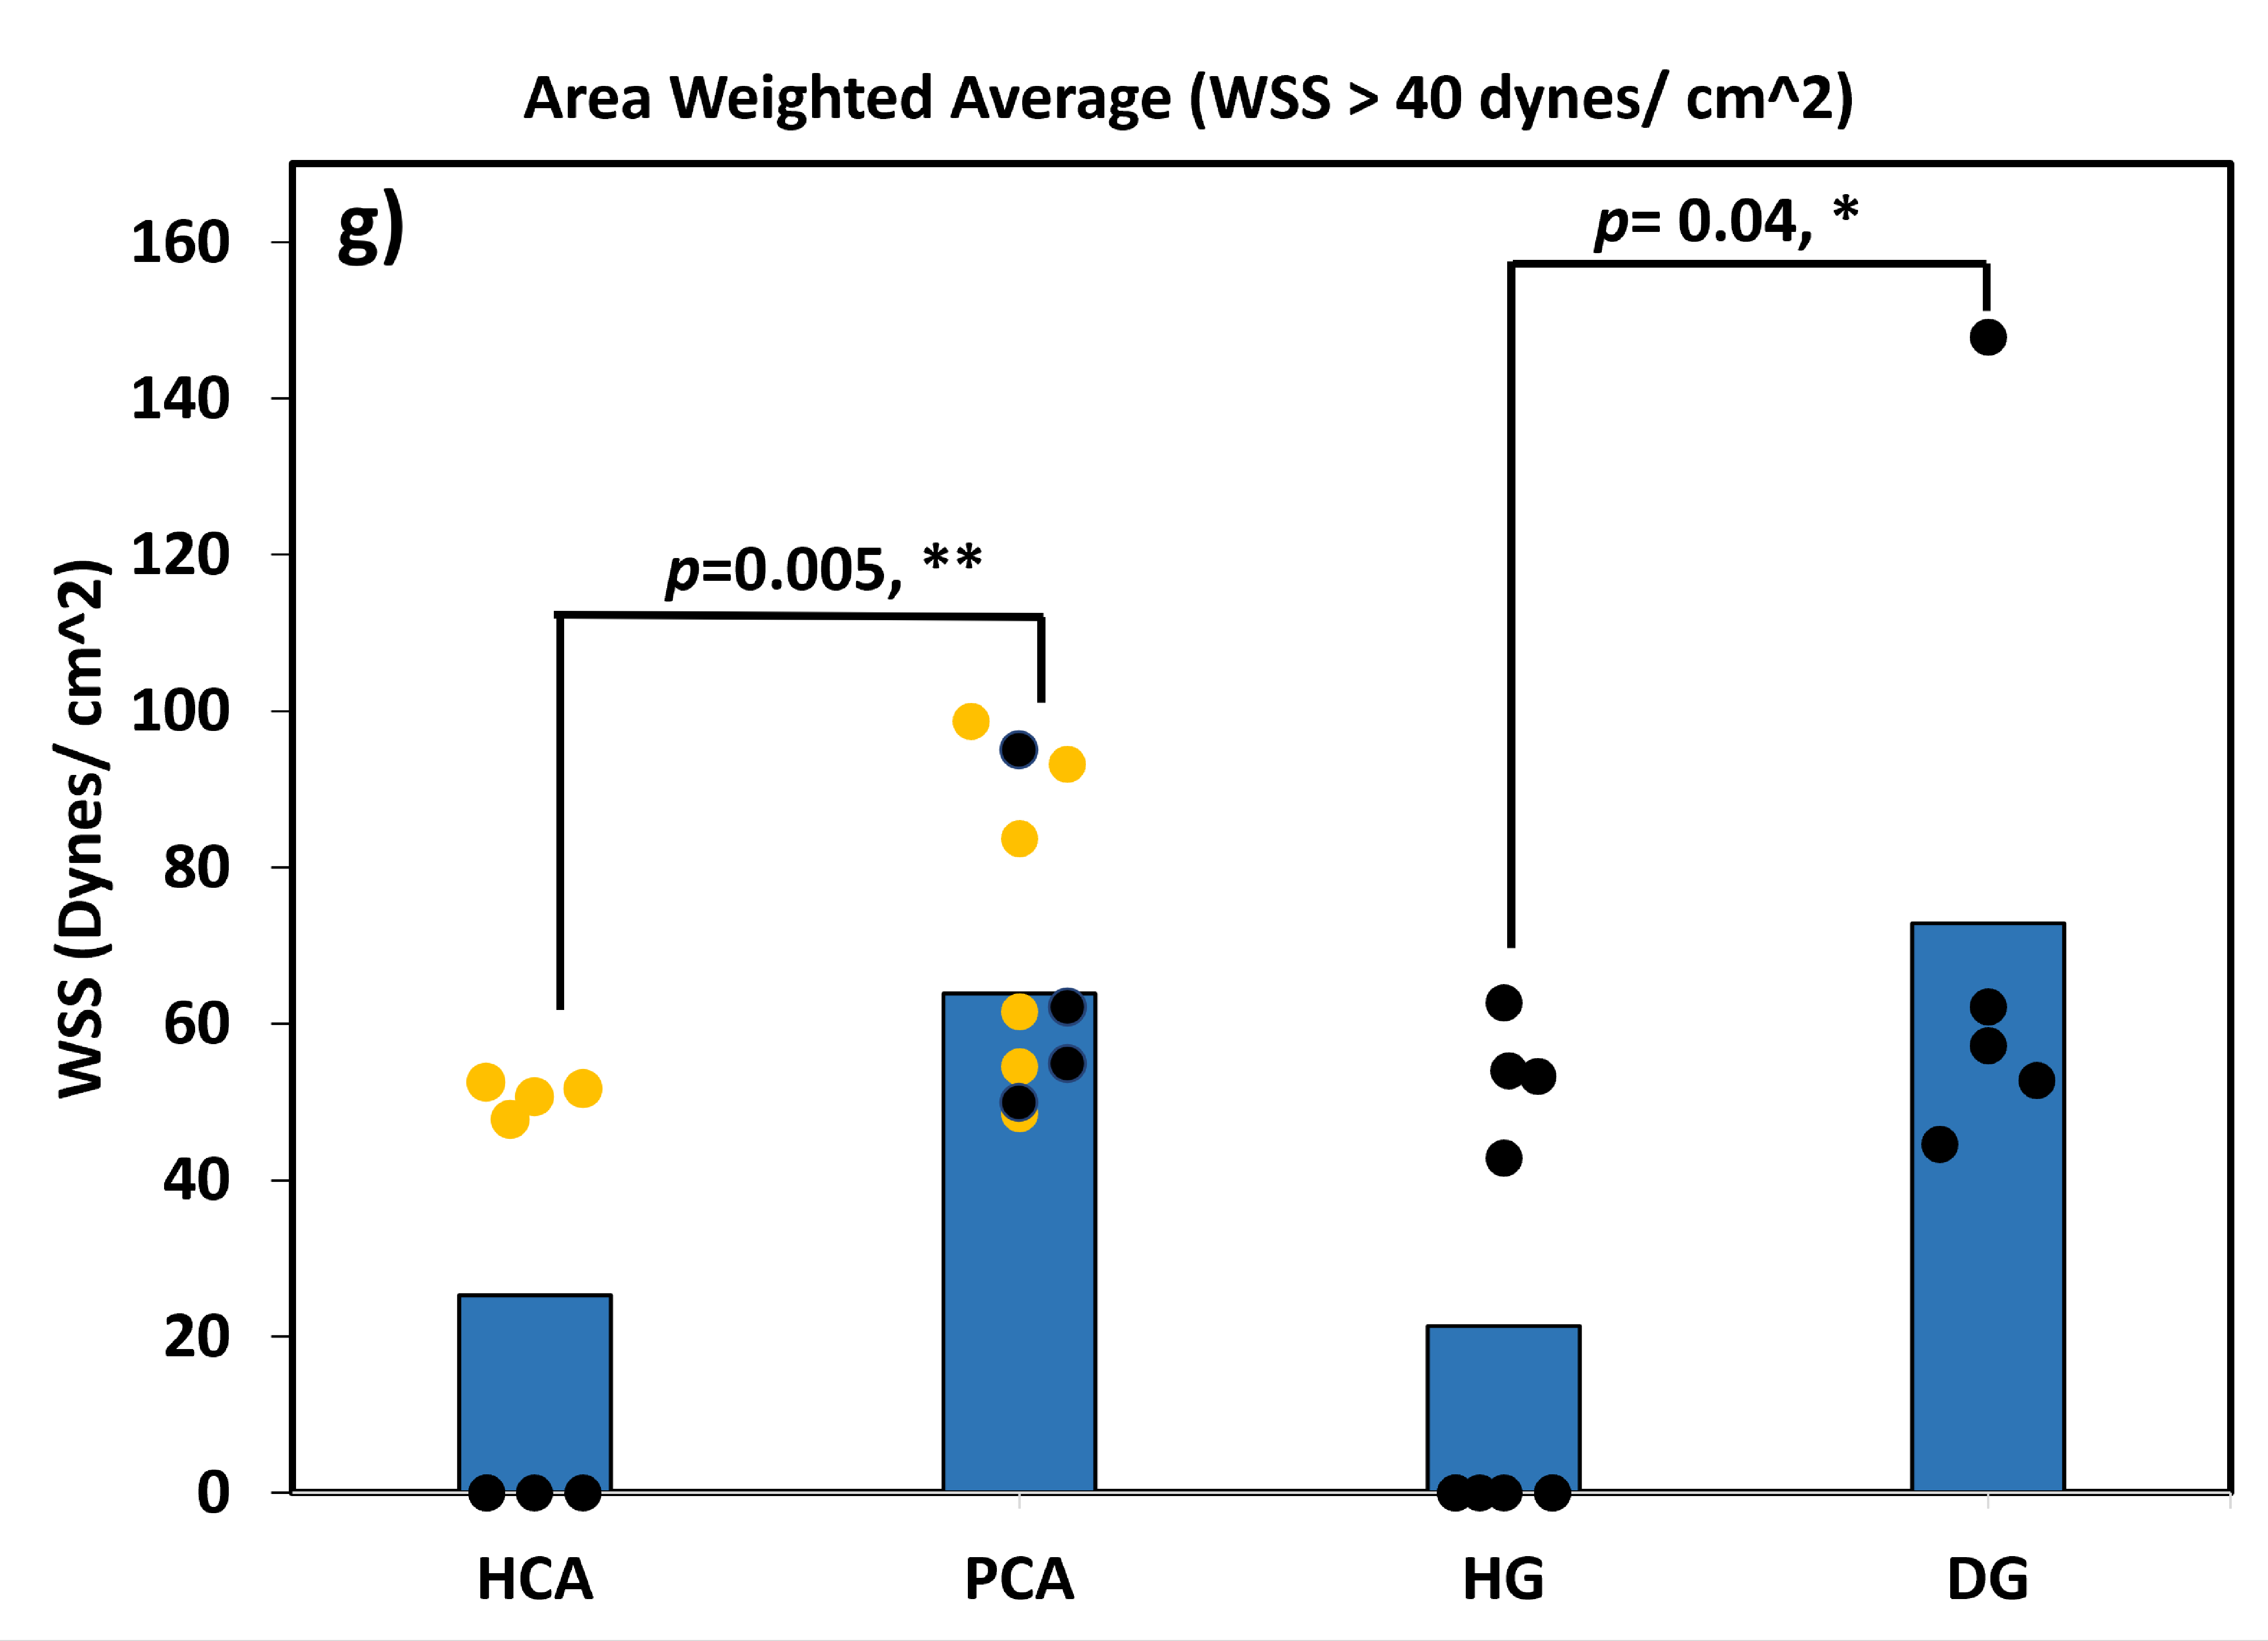
\includegraphics[width=9cm,height=7cm]{Newtonian AWAWSS Greater than 40 (1) (1).pdf}
    \end{subfigure}
    \hspace{1cm}
    \begin{subfigure}[d]{0.5\textwidth}
        \centering
        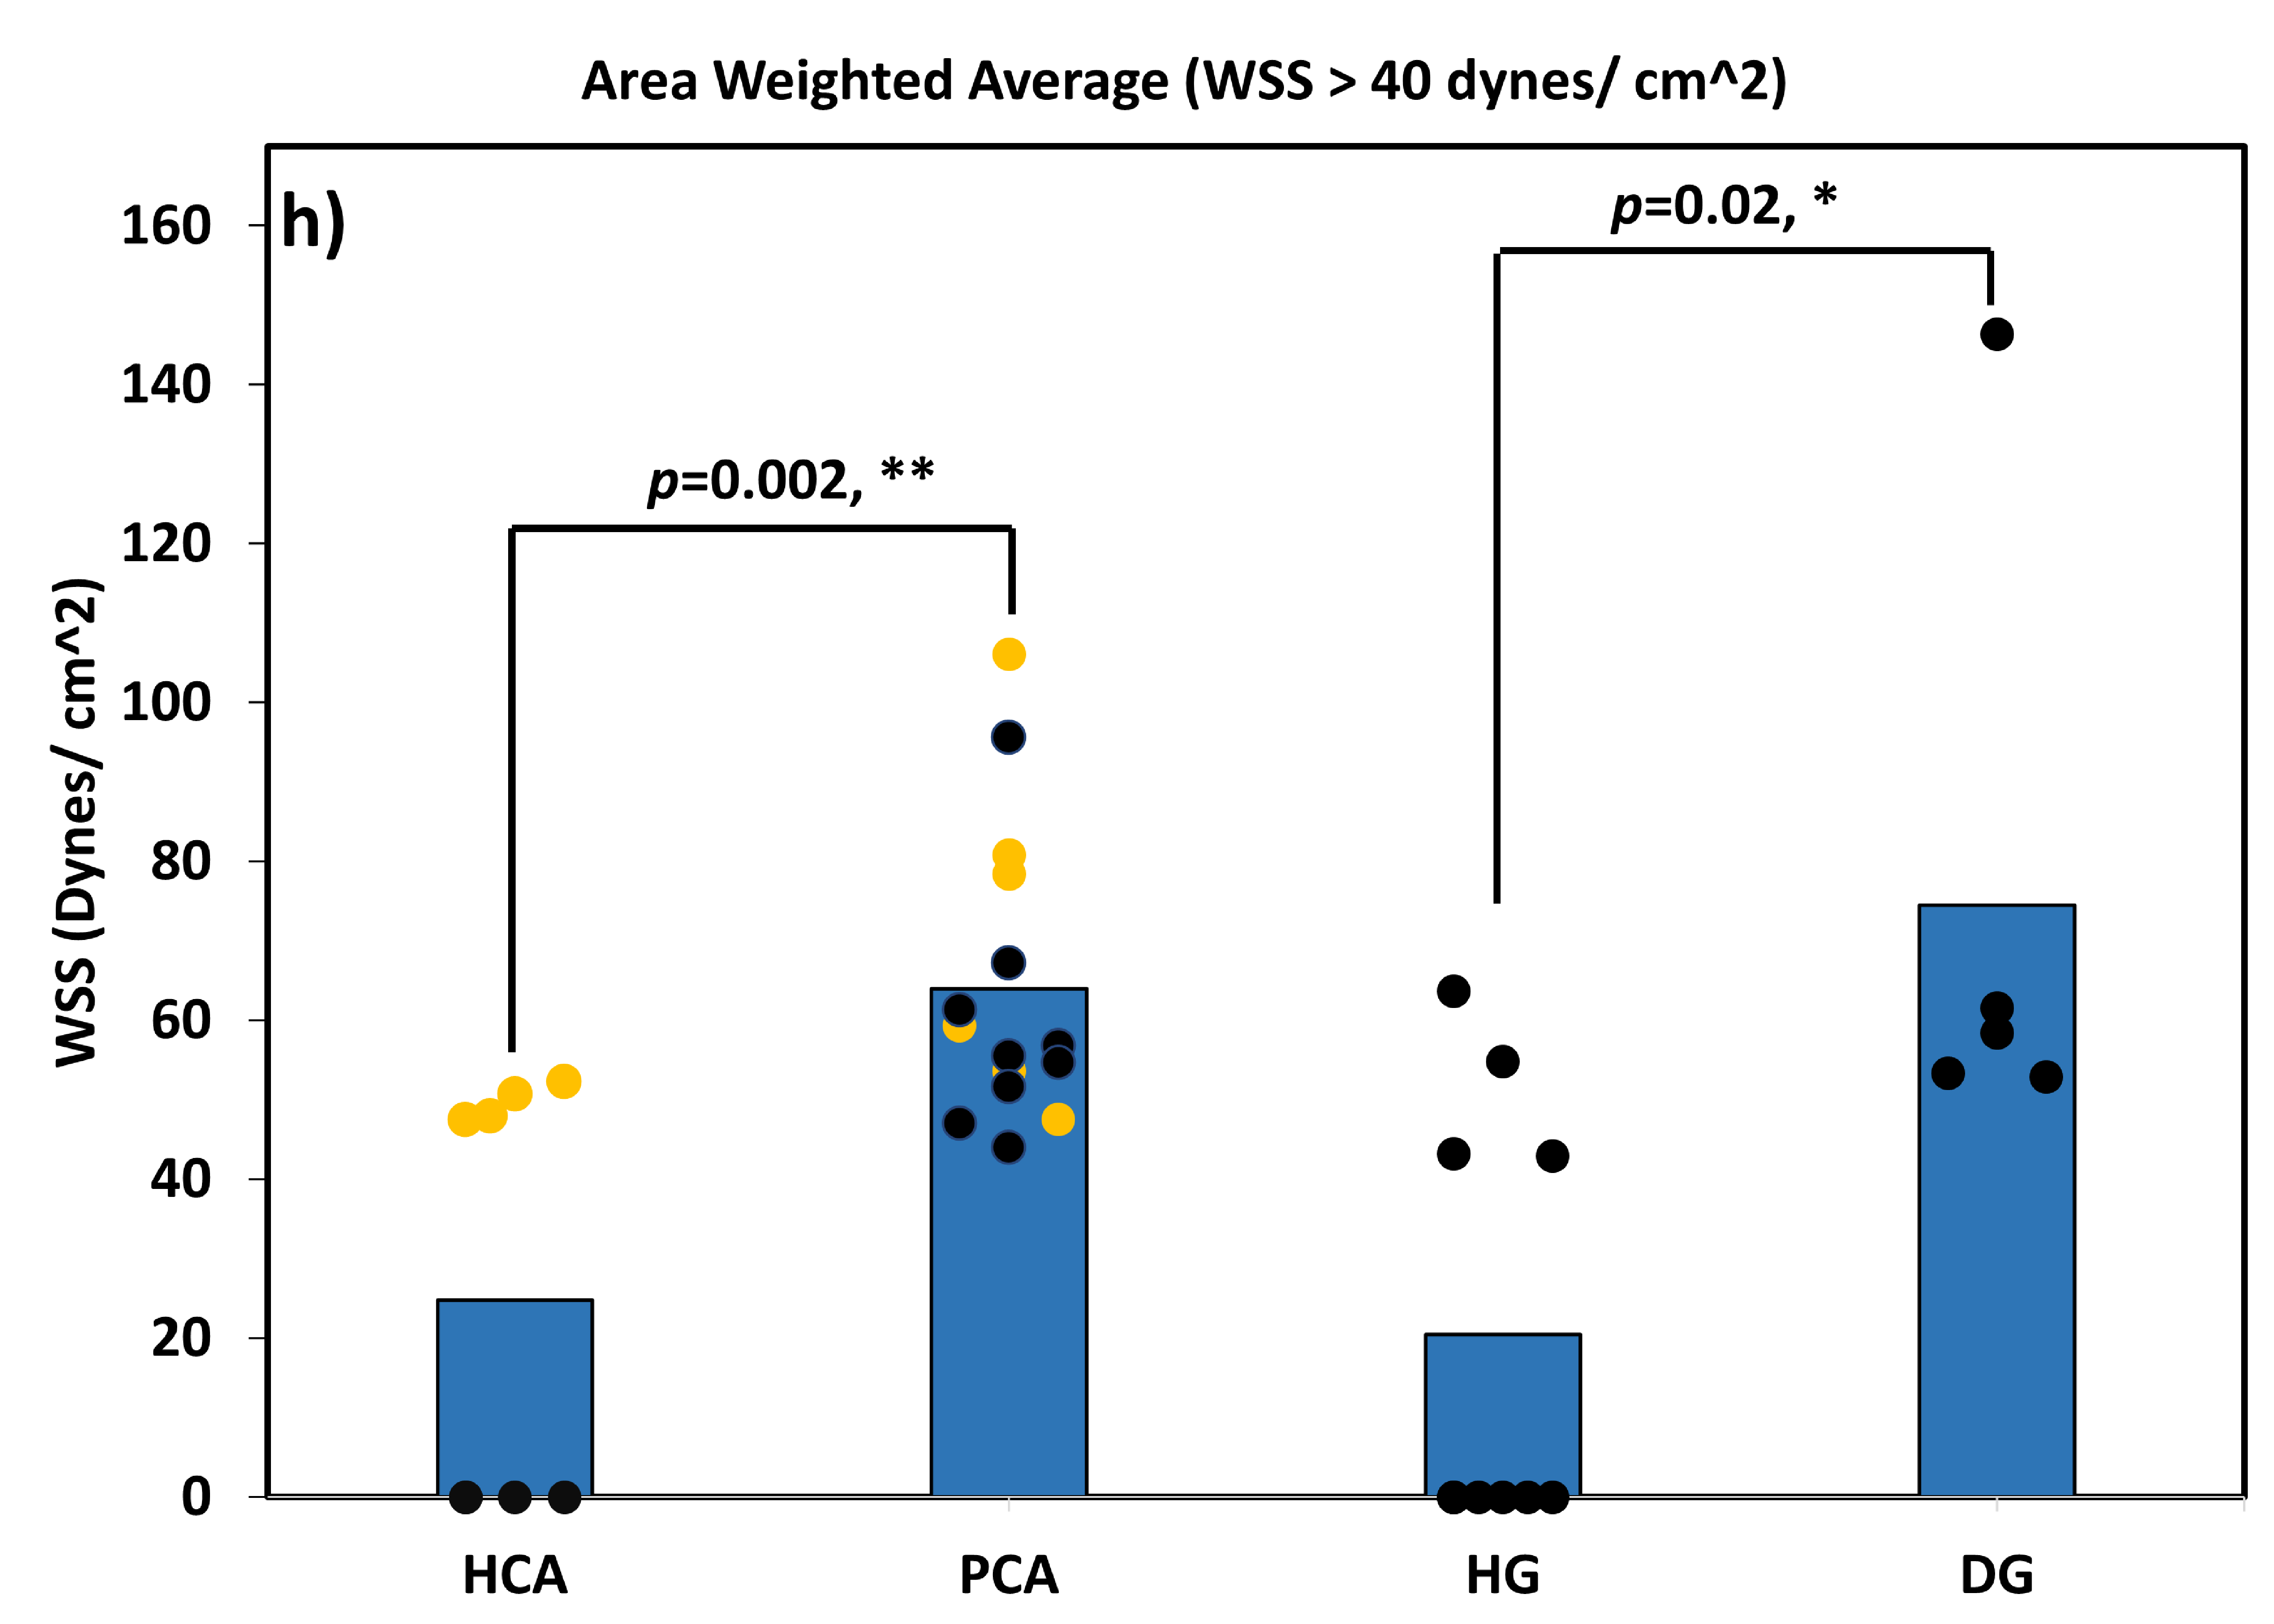
\includegraphics[width=9cm,height=7cm]{Carreau AWAWSS Greater than 40 (1) (1).pdf}
    \end{subfigure}
    \\
    \hspace{-2cm}
    \begin{subfigure}[d]{0.5\textwidth}
        \centering
        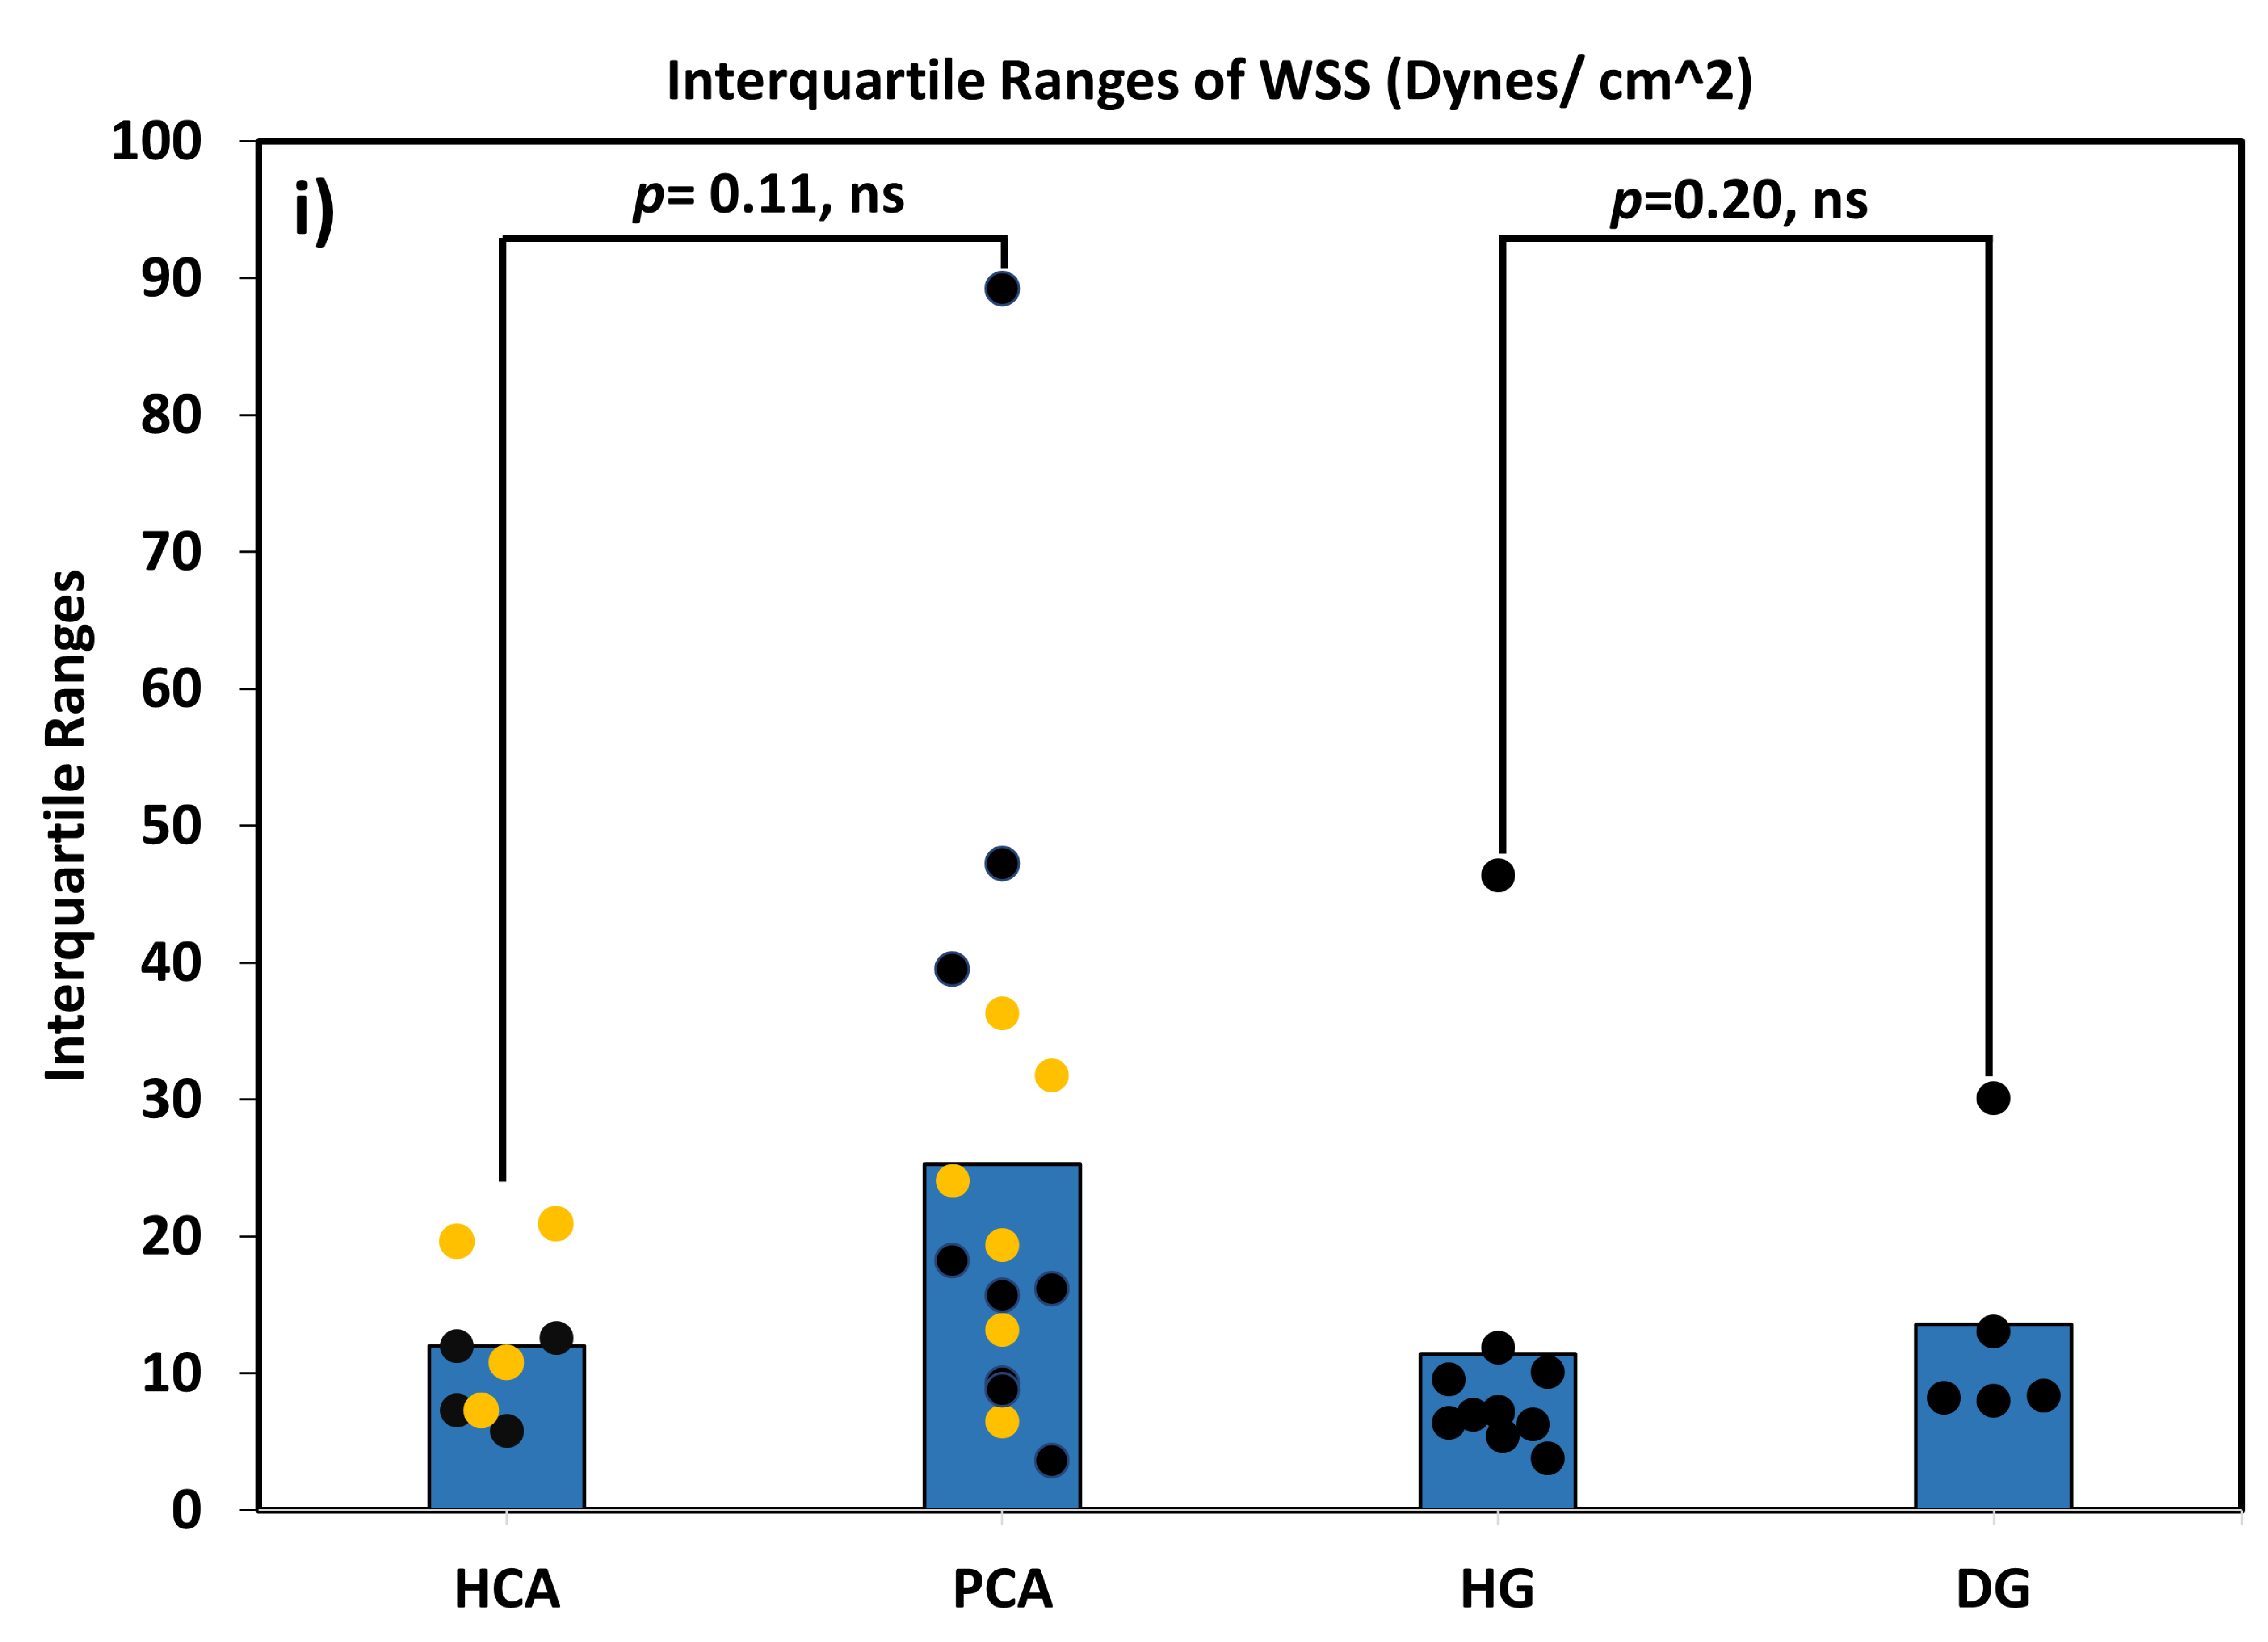
\includegraphics[width=9cm,height=7cm]{Newtonain ICR (1) (1).pdf}
    \end{subfigure}
    \hspace{1cm}
    \centering
    \begin{subfigure}[c]{0.5\textwidth}
        \centering
        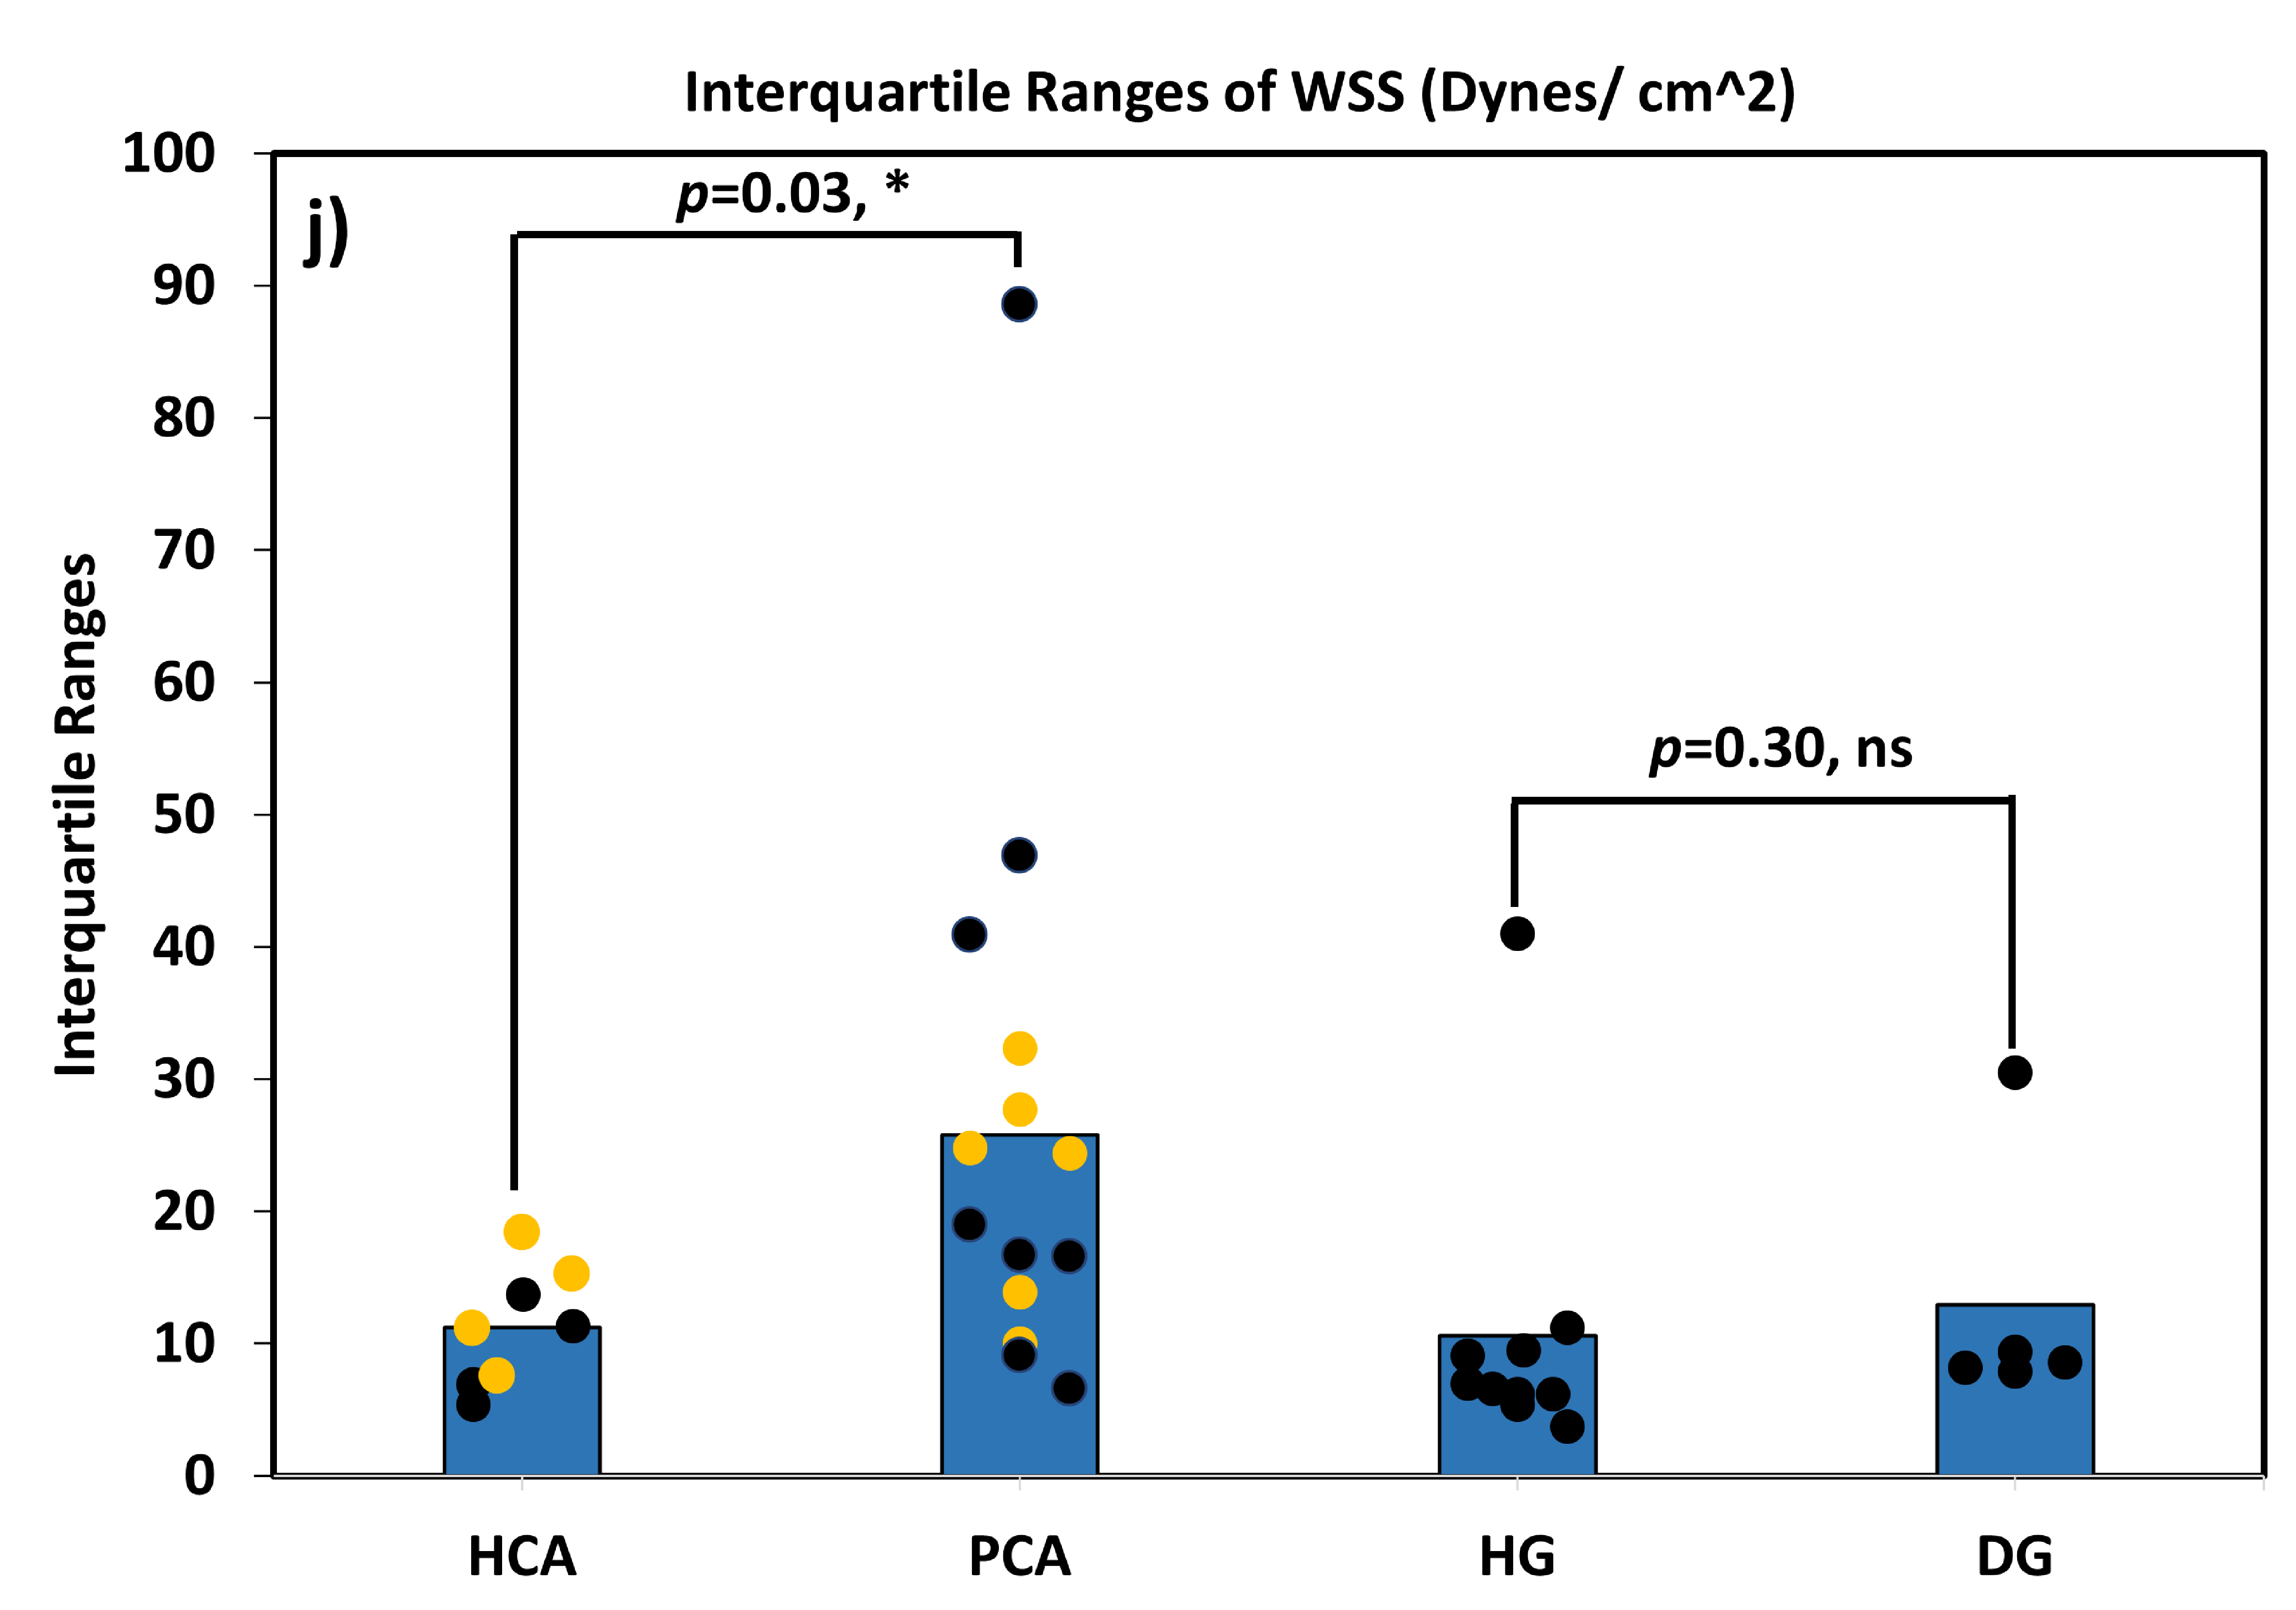
\includegraphics[width=9cm,height=7cm]{Carreau AWAWSS ICA (1) (1).pdf}
    \end{subfigure}
    \caption{Comparison of parameters between healthy and diseased vessels, with black points representing data from the Vascular Model Respiratory dataset and yellow points representing data from the ASOCA dataset. The parameters shown are: a) \& b) Area-weighted average WSS, c) \& d) Average WSS at bifurcations, e) \& f) Area fraction, g) \& h) Area-weighted average WSS greater than 40 dynes/cm$^2$, and i) \& j) Interquartile range of area-weighted average WSS.}
    \label{fig:3} 
\end{figure}

In overall, our analyses revealed differences between coronary arteries of healthy controls and patients with CAD and also between diseased and healthy grafts of CABG patients. While high WSS values were were mostly localized to bifurcations and maximally stenotic zones, they could also be present in other areas outside the primary stenosis, depending on overall arterial geometry changes. Wall area fraction exposed to high WSS above 40 dynes/ cm$^2$ was higher in diseased arteries and grafts, and these high-risk zones are mostly scattered at multiple points. We also noticed that WSS values could focally increase to very high values, that would not be obvious when overall overage WSS are calculated along arteries. These high WSS values were more sensitively detected with the Carreau-Yasuda model, indicating the importance of non-Newtonian models for assessing WSS of complex and disturbed flow dynamics in arterial geometries affected by atherosclerotic changes. The increased WSS in PCAs and DGs reflects abnormal flow dynamics caused by stenosis or atherosclerosis, conditions that disrupt smooth laminar flow and elevate shear forces on vessel walls. Detection of zones with high WSS can be important to assess the risk for plaque vulnerability during follow up of patients, that can lead to a severe graft failure and acute myocardial infarction. 


Previous studies, including those by Khan et al. \cite{3}, have linked low WSS to plaque progression and stenosis in SVGs. These studies evaluated parameters such as time-averaged WSS, oscillatory shear index (OSI), local and vessel-averaged WSS, normalized WSS (WSS*), low shear area (LSA), and flow rate. They found that WSS* was significantly lower in pre-diseased SVG segments compared to control segments without disease. While these findings are consistent with other research associating very low WSS with atherosclerotic plaque formation \cite{33, 42, 49, 50}, these studies did not observe differences in average WSS values between healthy and diseased grafts, nor did they provide detailed analysis of high WSS zones. Our study, however, aimed to identify differences in WSS distribution between healthy and diseased conditions relevant to CAD and SVGs, rather than to detect potential zones of plaque development or restenosis based on WSS values. This was due to the lack of longitudinal prospective imaging data. Instead of simply comparing WSS measurements averaged across entire arteries, we analyzed bifurcation and non-bifurcation areas separately, setting a threshold to identify and quantify focal zones of high WSS. This approach revealed that, compared to healthy controls, the right and left coronary arteries of CAD patients had a higher fraction of zones with WSS greater than 40 dynes/cm$^2$. The average WSS in these "hot-spot" zones was significantly higher, and the average WSS at bifurcations specifically was also elevated, even though overall average WSS values did not differ significantly. Furthermore, the same distinction was observed when comparing healthy and diseased saphenous vein grafts.


\subsubsection{Correlation Analysis}
\subsubsubsection{Correlation analysis in Newtonian Model:}
The correlation matrices are visualized as heat maps (Table~\ref{tableheatmapnewtonian}). Pearson correlation analysis revealed several strong and moderate relationships among the hemodynamic variables. In particular, a strong positive correlation was observed between the flow rates in Graft~2 (healthy, Graft~2(H)) and Graft~3 (diseased, Graft~3(D)) (\(r = 0.94\), \(p < 0.05\)), indicating closely coupled hemodynamic behavior of these grafts following coronary artery bypass surgery. In addition, inlet diameter and inlet velocity exhibited a very strong positive correlation (\(r = 0.99\)), reflecting their direct proportional relationship in the normalized geometric models.



With respect to WSS, strong positive relationships have been established with costs in Graft 2(H) (r = 0.71) and Graft 3(D) (r = 0.75), suggesting that increased volume costs in these grafts contribute to the growth of WSS, especially in affected segments. Moderate negative correlations with costs in RCA (r = -0.27) and LCA (r = -0.28) indicate a compensatory decrease in WSS in native arteries with an increase in local costs. Correlations with the diameter and speed of the entrance turned out to be weak and positive (r = 0.03 and r = 0.06, respectively), and with Graft 1(H) weakly positive (r = 0.23). The overall spectrum of correlations with WSS varies from weak to strong, with a predominance of positive relationships with costs in grafts (average |r| for WSS = 0.33).

\begin{table}[h!]
\centering
\caption{Correlation Matrix: Newtonian Model}
\resizebox{\textwidth}{!}{
\begin{tabular}{lcccccccc}
\hline
 & Inlet Diameter & Inlet & RCA & LCA & Graft 1 (H) & Graft 2 (H) & Graft 3 (D) & WSS \\
\hline
Inlet Diameter & \cellcolorcorr{1.00}1.00 & \cellcolorcorr{0.99}0.99 & \cellcolorcorr{0.58}0.58 & \cellcolorcorr{-0.28}-0.28 & \cellcolorcorr{-0.39}-0.39 & \cellcolorcorr{0.33}0.33 & \cellcolorcorr{0.25}0.25 & \cellcolorcorr{0.03}0.03 \\
Inlet          & \cellcolorcorr{0.99}0.99 & \cellcolorcorr{1.00}1.00 & \cellcolorcorr{0.60}0.60 & \cellcolorcorr{-0.29}-0.29 & \cellcolorcorr{-0.39}-0.39 & \cellcolorcorr{0.34}0.34 & \cellcolorcorr{0.26}0.26 & \cellcolorcorr{0.06}0.06 \\
RCA            & \cellcolorcorr{0.58}0.58 & \cellcolorcorr{0.60}0.60 & \cellcolorcorr{1.00}1.00 & \cellcolorcorr{-0.06}-0.06 & \cellcolorcorr{-0.39}-0.39 & \cellcolorcorr{0.14}0.14 & \cellcolorcorr{-0.02}-0.02 & \cellcolorcorr{-0.27}-0.27 \\
LCA            & \cellcolorcorr{-0.28}-0.28 & \cellcolorcorr{-0.29}-0.29 & \cellcolorcorr{-0.06}-0.06 & \cellcolorcorr{1.00}1.00 & \cellcolorcorr{-0.31}-0.31 & \cellcolorcorr{-0.32}-0.32 & \cellcolorcorr{0.49}0.49 & \cellcolorcorr{-0.28}-0.28 \\
Graft 1 (H)    & \cellcolorcorr{-0.39}-0.39 & \cellcolorcorr{-0.39}-0.39 & \cellcolorcorr{-0.39}-0.39 & \cellcolorcorr{-0.31}-0.31 & \cellcolorcorr{1.00}1.00 & \cellcolorcorr{0.40}0.40 & \cellcolorcorr{0.44}0.44 & \cellcolorcorr{0.23}0.23 \\
Graft 2 (H)    & \cellcolorcorr{0.33}0.33 & \cellcolorcorr{0.34}0.34 & \cellcolorcorr{0.14}0.14 & \cellcolorcorr{-0.32}-0.32 & \cellcolorcorr{0.40}0.40 & \cellcolorcorr{1.00}1.00 & \cellcolorcorr{0.94}0.94 & \cellcolorcorr{0.71}0.71 \\
Graft 3 (D)    & \cellcolorcorr{0.25}0.25 & \cellcolorcorr{0.26}0.26 & \cellcolorcorr{-0.02}-0.02 & \cellcolorcorr{0.49}0.49 & \cellcolorcorr{0.44}0.44 & \cellcolorcorr{0.94}0.94 & \cellcolorcorr{1.00}1.00 & \cellcolorcorr{0.75}0.75 \\
WSS            & \cellcolorcorr{0.03}0.03 & \cellcolorcorr{0.06}0.06 & \cellcolorcorr{-0.27}-0.27 & \cellcolorcorr{-0.28}-0.28 & \cellcolorcorr{0.23}0.23 & \cellcolorcorr{0.71}0.71 & \cellcolorcorr{0.75}0.75 & \cellcolorcorr{1.00}1.00 \\
\hline
\end{tabular}
}
\label{tableheatmapnewtonian}
\end{table}

Thus, these results reflect key aspects of hemodynamics in the post-CABG patient: increased flow in the SVG, especially in those affected by stenosis (Graft 3(D)), contributes to the local increase in WSS, which corresponds to the mechanisms of atherosclerosis progression. High WSS activates endothelial signaling cascades, including matrix metalloproteinases (MMPs), leading to the degradation of the fibrous capsule of plaques and increasing the risk of acute rupture \cite{10.1093/rb/rbw021}. Negative correlations with arterial flow illustrate the body's adaptive response: a decrease in flow in the RCA/LCA compensates for hyperflow in the grafts, preventing diffuse endothelial stress but increasing the local risk of thrombosis in the shunts. This highlights the vulnerability of SVGD, where the Newtonian model, by ignoring the dependence of blood viscosity on shear rate, underestimates the biological sensitivity to nonlinear effects such as endothelial apoptosis and intraplaque hemorrhage, which is consistent with clinical observations.

From the point of view of hydrodynamics, these results illustrate the fundamental principles of laminar and transient flows in branching vessels: positive correlations with flow rates in grafts reflect an increased velocity gradient in the zones of constriction and curvature, where Newtonian viscosity ($\mu = \text{const}$) leads to a quadratic increase in WSS, especially in the poststenotic segments of Graft 3(D). This corresponds to the Bernoulli effect in local flow accelerations, where increased flow generates turbulent vortices at the wall, increasing the OSI and contributing to unsteady fluctuations in the WSS. Negative correlations with arteries (RCA/LCA) demonstrate hydrodynamic compensation through pressure distribution: reducing flow in native branches minimizes recirculation zones, stabilizing flow according to the law of conservation of mass, but enhances the local hydrostatic gradient in shunts. In the Newtonian model assuming constant viscosity, such connections overestimate linear effects, leading to overestimated correlations by 10--15\% compared to real turbulent regimes (Re $>$ 1000), as noted in CFD simulations of coronary networks \cite{10.1016/j.ijnonlinmec.2020.103477}. This highlights the limitations of linear rheology in predicting high hydraulic displacement zones, where ignoring dynamic viscosity leads to errors in estimating the vortex structure of the flow.
 


\subsubsubsection{Correlation analysis in Carreau--Yasuda:}

In the non--Newtonian Carreau--Yasuda model (Table~\ref{tableheatmapcarreau}), strong positive correlations are confirmed between expenses in Graft 2(H) and Graft 3(D) (r = 0.91; p < 0.05), as well as moderate positive associations of these expenses with WSS (r = 0.62 for Graft 2(H) and r = 0.66 for Graft 3(D)), emphasizing the increased sensitivity of the model to nonlinear viscosity effects in high-risk areas. The ideal correlation between Inlet Diameter and Inlet Velocity is preserved (r = 0.99).

The correlations of WSS with RCA (r = -0.26) and LCA (r = -0.26) remain moderately negative, similar to the Newtonian model, indicating a stabilizing effect in the arteries. Weak positive bonds are observed with Graft 1(H) (r = 0.12), and weak negative ones with the diameter and speed of entry (r = -0.02 and r = -0.03, respectively). In contrast to the Newtonian model, here correlations with expenses in graphs show a less pronounced positive trend, with moderate values for the affected segments (average |r| for WSS = 0.28).

\begin{table}[h!]
\centering
\caption{Correlation Matrix: Carreau--Yasuda Model}
\resizebox{\textwidth}{!}{
\begin{tabular}{lcccccccc}
\hline
 & Inlet Diameter & Inlet & RCA & LCA & Graft 1 (H) & Graft 2 (H) & Graft 3 (D) & WSS \\
\hline
Inlet Diameter & \cellcolorcorr{1.00}1.00 & \cellcolorcorr{0.99}0.99 & \cellcolorcorr{0.65}0.65 & \cellcolorcorr{-0.30}-0.30 & \cellcolorcorr{-0.45}-0.45 & \cellcolorcorr{0.38}0.38 & \cellcolorcorr{0.21}0.21 & \cellcolorcorr{-0.02}-0.02 \\
Inlet          & \cellcolorcorr{0.99}0.99 & \cellcolorcorr{1.00}1.00 & \cellcolorcorr{0.67}0.67 & \cellcolorcorr{-0.31}-0.31 & \cellcolorcorr{-0.42}-0.42 & \cellcolorcorr{0.33}0.33 & \cellcolorcorr{0.18}0.18 & \cellcolorcorr{-0.03}-0.03 \\
RCA            & \cellcolorcorr{0.65}0.65 & \cellcolorcorr{0.67}0.67 & \cellcolorcorr{1.00}1.00 & \cellcolorcorr{-0.05}-0.05 & \cellcolorcorr{-0.43}-0.43 & \cellcolorcorr{0.19}0.19 & \cellcolorcorr{-0.05}-0.05 & \cellcolorcorr{-0.26}-0.26 \\
LCA            & \cellcolorcorr{-0.30}-0.30 & \cellcolorcorr{-0.31}-0.31 & \cellcolorcorr{-0.05}-0.05 & \cellcolorcorr{1.00}1.00 & \cellcolorcorr{-0.15}-0.15 & \cellcolorcorr{-0.36}-0.36 & \cellcolorcorr{0.31}0.31 & \cellcolorcorr{0.12}0.12 \\
Graft 1 (H)    & \cellcolorcorr{-0.45}-0.45 & \cellcolorcorr{-0.42}-0.42 & \cellcolorcorr{-0.43}-0.43 & \cellcolorcorr{-0.15}-0.15 & \cellcolorcorr{1.00}1.00 & \cellcolorcorr{0.66}0.66 & \cellcolorcorr{0.10}0.10 & \cellcolorcorr{0.62}0.62 \\
Graft 2 (H)    & \cellcolorcorr{0.38}0.38 & \cellcolorcorr{0.33}0.33 & \cellcolorcorr{0.19}0.19 & \cellcolorcorr{-0.36}-0.36 & \cellcolorcorr{0.66}0.66 & \cellcolorcorr{1.00}1.00 & \cellcolorcorr{0.91}0.91 & \cellcolorcorr{0.60}0.60 \\
Graft 3 (D)    & \cellcolorcorr{0.21}0.21 & \cellcolorcorr{0.18}0.18 & \cellcolorcorr{-0.05}-0.05 & \cellcolorcorr{0.31}0.31 & \cellcolorcorr{0.10}0.10 & \cellcolorcorr{0.91}0.91 & \cellcolorcorr{1.00}1.00 & \cellcolorcorr{0.66}0.66 \\
WSS            & \cellcolorcorr{-0.02}-0.02 & \cellcolorcorr{-0.03}-0.03 & \cellcolorcorr{-0.26}-0.26 & \cellcolorcorr{0.12}0.12 & \cellcolorcorr{0.62}0.62 & \cellcolorcorr{0.60}0.60 & \cellcolorcorr{0.66}0.66 & \cellcolorcorr{1.00}1.00 \\
\hline
\end{tabular}
}
\label{tableheatmapcarreau}
\end{table}

Thus, this illustrates the advantage of taking into account the non-Newtonian behavior of blood (reduction of viscosity at high shear), which enhances WSS in the stenotic zones of grafts, simulating real conditions of hypercoagulation and endothelial dysfunction. Moderate correlations with WSS in affected grafts (Graft 3(D)) correlate with the mechanisms of plaques vulnerability: a high shift provokes activation of the NF-kB pathway, promoting inflammation and apoptosis, which leads to acute coronary syndrome \cite{10.1016/j.vph.2024.107452}. Negative correlation with arteries suggest a protective effect in native vessels, where low flow minimizes oxidative stress, but in grafts it increases the risk, especially in patients with diffuse atherosclerosis. In contrast to the Newtonian model, Carreau--Yasuda better reproduces experimental data on elevated WSS in bifurcations associated with plaque rupture \cite{10.3389/fphys.2025.1509875} and explains why patients with SVG show a more aggressive disease progression compared to arterial shunts, emphasizing the need for personalized monitoring for the progression of atherothrombosis.

Hydrodynamically, this demonstrates the role of dynamic viscosity in the nonlinear rheology of blood: increased correlations with WSS in grafts (Graft 3(D)) are due to a decrease in $\dot{\gamma} > 100 \,\text{s}^{-1}$, which enhances the velocity gradient in the stenotic zones, leading to an exponential growth of $\tau_w$ and the formation of secondary flows in the curved segments. The Carreau--Yasuda model captures the pseudoplasticity of blood as a suspension better, where local viscosity dilution ($\eta_0 \rightarrow \eta_\infty$) enhances convective pulse transport, increasing local WSS peaks by 15--25\% in bifurcations compared to the Newtonian approximation. The negative connections with the arteries illustrate hydrodynamic adaptation: in RCA/LCA, low flow contributes to the laminar Poiseuille profile, minimizing viscous dissipation, whereas in grafts nonlinear viscosity enhances turbulent diffusion, generating pressure fluctuations and vortex cores at the wall. This is consistent with experimental PIV data on coronary flow, where non--Newtonian models more accurately reproduce the zones of recirculation and increased OSI ($>$0.1) in shunts \cite{10.1016/j.jbiomech.2005.01.034}, explaining a higher sensitivity to geometric defects (stenoses of 50--70\%), such as an increase in hydraulic resistance. Thus, the model reveals hydrodynamic mechanisms where the nonlinearity of viscosity enhances the unsteadiness of the flow, improving the prediction of risk zones.

\subsubsubsection{Comparison of viscosity models:}

Comparison of correlation matrices revealed similarities in strong relationships between graft flow rates (r $>$ 0.90 in both models), but the Newtonian model demonstrates stronger positive correlations of WSS with Graft 2(H) and Graft 3(D) (0.71--0.75) compared to the Carreau--Yasuda (0.62--0.66), reflecting overestimation of linear effects under constant viscosity conditions. Negative correlations with arterial flows (RCA, LCA) are almost identical (r $\approx$ -0.26-- -0.28), while the correlations with input parameters remain weak in both models. In general, the non--Newtonian model demonstrates lower variability of correlations with WSS (std = 0.24 vs. 0.27 in the Newtonian model), which confirms its advantage in identifying hemodynamic risks due to its realistic account of nonlinearity (the average |r| for WSS is $\sim$15\% lower). These differences highlight the role of nonlinear viscosity in enhancing the predictive power of the analysis, despite the apparent "strength" of correlations in the Newtonian model.

Biologically, the differences in the models illustrate the critical role of shear-rate-dependent viscosity in predicting vascular pathology: Carreau--Yasuda enhances the detection of high WSS zones in grafts, reflecting the actual physiology of blood as a suspension of red blood cells, where a decrease in viscosity at shear rates $>$100 s$^{-1}$ enhances endothelial stress and thrombogenesis \cite{10.3389/fphys.2020.00861}. This is consistent with the finding that the Newtonian model overestimates correlations but underestimates the risk of plaque rupture by 20--30\% in stenoses \cite{10.1136/neurintsurg-2011-010089}, while the non--Newtonian model better correlates with clinical outcomes such as acute SVG occlusion. The increased predictive power in affected grafts highlights the biological vulnerability of post-CABG patients to asymmetric vascular remodeling, where high WSS in the shunts provokes local atherothrombosis, in contrast to arteries where compensatory mechanisms (e.g., vasodilation) mitigate the effect. These findings justify the transition to non--Newtonian models for accurate risk assessment.


From a hydrodynamic perspective, the differences in the models highlight the transition from linear (Newtonian: constant $\mu$) to nonlinear rheology (Carreau--Yasuda: $\eta(\dot{\gamma})$), where stronger correlations in the Newtonian model reflect a simplified assessment of viscous dissipation in high-shear regimes: in stenoses, the constant viscosity enhances inertial forces (local Re $\rightarrow \infty$), leading to turbulent bursts and an increase in turbulent kinetic energy ($k$) in the $k$-$\omega$ SST model. Stable negative connections with arteries demonstrate the universality of the Darcy--Weisbach law for laminar branches, where both models predict minimal gradients, but Carreau--Yasuda model more accurately simulates the transition to turbulence in shunts (critical Re $\approx 2000$). Lower variability in the non--Newtonian model indicates its ability to capture asymmetric velocity profiles and increased local WSS by 20\%. This confirms the experimental CFD data on the Newtonian model's overestimation of dissipation in bifurcations \cite{10.1007/s42452-020-03561-w}, where ignoring the dependence of viscosity on shear rate distorts the balance of forces (inertia vs viscosity), leading to errors in predicting secondary flows and hydraulic resistance. As a result, the transition to the Carreau--Yasuda model is justified for accurately modeling mixed flow regimes in CABG systems, improving the estimation of energy losses and hydrodynamic stress zones.


\subsection{\label{PINN Results}{Physics-Informed Neural Network Results}}

\hspace*{\parindent}
\addp{We trained PINN surrogate models on CFD data from twelve patient cases representing healthy, diseased, and SVG categories. For every patient, rheology-matched physics losses produce a Newtonian surrogate trained against the Newtonian CFD and a Carreau--Yasuda surrogate trained against the Carreau--Yasuda CFD. To distinguish predictive from interpolative accuracy as recommended by the reviewers, each surrogate is evaluated under a per-patient spatial holdout in which 20\% of the mesh points are withheld from training under a fixed random seed and used solely for evaluation. The training-fit (interpolation) and held-out (prediction) values are summarised in Table~\ref{tab:pinn_holdout} for the Newtonian surrogate and in Table~\ref{tab:pinn_holdout_cy} for the Carreau--Yasuda surrogate. Both tables report three metrics. The Normalized Root Mean Square Error (NRMSE) expresses error as a percentage of the patient-specific WSS range, allowing comparison across geometries. The coefficient of determination $R^2$ measures the proportion of CFD variance explained by the surrogate. The Pearson correlation coefficient $r$ is reported on the held-out subset. The held-out subset is a uniform random sample of the same vasculature and directly probes the surrogate's ability to predict at locations on the same patient that it has not seen during training.}

\begin{table}[!htbp]
\color{red}% mark this entire table as a revision-stage addition
\centering
\setlength{\tabcolsep}{4pt}
\renewcommand{\arraystretch}{0.95}
\caption{\textcolor{red}{PINN held-out performance under a per-patient spatial holdout (20\% of mesh points withheld with a fixed seed). Metrics are reported on the training subset (interpolation) and on the held-out subset (prediction); the latter quantifies the surrogate's ability to predict at unseen locations on the same vasculature.}}
\label{tab:pinn_holdout}
\begin{tabular}{|c|c|c|c|c|c|c|}
\hline
\multirow{2}{*}{\textbf{Patient}} & \multirow{2}{*}{\textbf{Category}} & \multicolumn{2}{c|}{\textbf{NRMSE (\%)}} & \multicolumn{2}{c|}{\textbf{$R^2$}} & \textbf{Pearson $r$} \\
\cline{3-6}
 & & Train & Holdout & Train & Holdout & Holdout \\
\hline
H1 & Healthy & 2.87 & 2.83 & 0.691 & 0.714 & 0.946 \\
H2 & Healthy & 3.60 & 3.52 & 0.419 & 0.413 & 0.871 \\
H3 & Healthy & 1.54 & 2.41 & 0.708 & 0.693 & 0.899 \\
H4 & Healthy & 0.91 & 0.84 & 0.908 & 0.911 & 0.971 \\
BG1 & SVG & 2.48 & 2.53 & 0.766 & 0.755 & 0.923 \\
BG2 & SVG & 1.36 & 1.55 & 0.721 & 0.736 & 0.909 \\
BG3 & SVG & 1.91 & 1.92 & 0.794 & 0.803 & 0.946 \\
BG4 & SVG & 3.44 & 3.74 & 0.836 & 0.839 & 0.945 \\
BG5 & SVG & 4.53 & 4.33 & 0.623 & 0.617 & 0.902 \\
D1 & Diseased & 2.14 & 2.37 & 0.803 & 0.801 & 0.938 \\
D2 & Diseased & 0.83 & 1.04 & 0.793 & 0.757 & 0.949 \\
D3 & Diseased & 2.51 & 2.46 & 0.800 & 0.803 & 0.934 \\
\hline
\textbf{Mean} & -- & \textbf{2.34} & \textbf{2.46} & \textbf{0.739} & \textbf{0.737} & \textbf{0.928} \\
\hline
\end{tabular}
\end{table}

\begin{table}[!htbp]
\color{red}% mark this entire table as a revision-stage addition
\centering
\setlength{\tabcolsep}{4pt}
\renewcommand{\arraystretch}{0.95}
\caption{\textcolor{red}{PINN held-out performance under the same per-patient spatial holdout (20\% of mesh points withheld with a fixed seed) for the Carreau--Yasuda surrogate. Same protocol and reporting convention as Table~\ref{tab:pinn_holdout}; gradient-norm-balanced loss weights are recomputed per patient from a Carreau--Yasuda forward pass.}}
\label{tab:pinn_holdout_cy}
\begin{tabular}{|c|c|c|c|c|c|c|}
\hline
\multirow{2}{*}{\textbf{Patient}} & \multirow{2}{*}{\textbf{Category}} & \multicolumn{2}{c|}{\textbf{NRMSE (\%)}} & \multicolumn{2}{c|}{\textbf{$R^2$}} & \textbf{Pearson $r$} \\
\cline{3-6}
 & & Train & Holdout & Train & Holdout & Holdout \\
\hline
H1 & Healthy & 3.97 & 3.95 & 0.403 & 0.380 & 0.909 \\
H2 & Healthy & 3.59 & 3.71 & 0.524 & 0.534 & 0.905 \\
H3 & Healthy & 5.19 & 5.50 & 0.611 & 0.609 & 0.897 \\
H4 & Healthy & 1.67 & 1.95 & 0.896 & 0.890 & 0.966 \\
BG1 & SVG & 3.69 & 4.65 & 0.903 & 0.902 & 0.968 \\
BG2 & SVG & 2.73 & 3.57 & 0.733 & 0.718 & 0.938 \\
BG3 & SVG & 3.54 & 3.70 & 0.815 & 0.785 & 0.949 \\
BG4 & SVG & 4.59 & 4.61 & 0.664 & 0.651 & 0.905 \\
BG5 & SVG & 2.74 & 2.98 & 0.825 & 0.829 & 0.959 \\
D1 & Diseased & 1.85 & 2.08 & 0.809 & 0.791 & 0.953 \\
D2 & Diseased & 2.53 & 3.46 & 0.727 & 0.707 & 0.902 \\
D3 & Diseased & 1.72 & 2.03 & 0.640 & 0.620 & 0.883 \\
\hline
\textbf{Mean} & -- & \textbf{3.15} & \textbf{3.52} & \textbf{0.713} & \textbf{0.701} & \textbf{0.928} \\
\hline
\end{tabular}
\end{table}

\addp{Across all twelve patients the held-out NRMSE and $R^2$ track the training values closely under both rheologies, indicating that the surrogate generalises within each patient's geometry rather than memorising the training mesh. For the Newtonian surrogate (Table~\ref{tab:pinn_holdout}) the mean train-versus-holdout values are NRMSE $2.34\%$ vs $2.46\%$ and $R^2$ $0.739$ vs $0.737$, and the held-out Pearson $r$ averages $0.928$. For the Carreau--Yasuda surrogate (Table~\ref{tab:pinn_holdout_cy}) the corresponding values are NRMSE $3.15\%$ vs $3.52\%$ and $R^2$ $0.713$ vs $0.701$, and the held-out Pearson $r$ averages $0.928$. Per-patient train-to-holdout drops in $R^2$ stay below $0.04$ in every case under both rheologies, and the held-out Pearson $r$ exceeds $0.87$ for every patient. The Carreau--Yasuda surrogate is uniformly slightly less accurate than the Newtonian one, with a mean NRMSE gap of about one percentage point. This reflects the additional non-linearity introduced by the strain-rate-dependent viscosity in both the momentum residual and the WSS-from-gradient consistency loss. The rheology-matched Pearson correlations are nonetheless close, confirming that the surrogate captures the spatial structure of WSS in both Newtonian and non-Newtonian regimes. These results directly address the interpolation-versus-prediction concern raised in the review. Under either rheology, the PINN predicts at unseen locations on the same vasculature with negligible accuracy loss compared with the training subset.}

% \hspace*{\parindent}
\addp{When the held-out errors are stratified by anatomical category, the Newtonian held-out NRMSE means are 2.40\% for healthy cases, 2.81\% for SVG cases, and 1.96\% for diseased cases. The corresponding Carreau--Yasuda means are 3.78\%, 3.90\%, and 2.52\%. The diseased category therefore achieves the lowest mean NRMSE under both rheologies despite its more complex flow patterns, primarily because diseased vessels have wider WSS dynamic ranges that reduce relative error. At the per-patient level, the lowest Newtonian NRMSE is obtained for H4 (0.84\%), which also attains the highest $R^2$ in that set (0.911). Under Carreau--Yasuda, BG1 attains the highest $R^2$ (0.902) and H4 again the lowest NRMSE (1.95\%).}

\addp{The observed performance variability across patients reflects differences in geometric complexity and WSS dynamic range. Healthy patients with narrow WSS ranges, notably H1 and H2, show comparatively higher NRMSE because the same absolute error becomes a larger relative quantity; the corresponding contour maps nonetheless show modest pointwise errors. SVG patients exhibit consistent performance across both rheologies (Newtonian NRMSE 1.55--4.33\%, Carreau--Yasuda 2.98--4.65\%), confirming that the surrogate captures multi-anastomosis bypass-graft hemodynamics. Together these results suggest that PINNs can reliably serve as surrogates for CFD across diverse coronary anatomies and rheological assumptions, from healthy vessels to severely diseased arteries and post-surgical grafts.}

\added[id=pinn]{The per-patient PINN performance under the spatial holdout is summarised graphically in Figure~\ref{fig:pinn_holdout_summary}.} Figure~\ref{fig:pinn_wss_h1} shows the H1 (Healthy) Newtonian comparison and Figure~\ref{fig:pinn_wss_svg_diseased} shows the BG2 (SVG) and D3 (Diseased) Newtonian comparisons, each in two orthogonal projections. \addp{Figures~\ref{fig:pinn_wss_h1_cy} and~\ref{fig:pinn_wss_svg_diseased_cy} repeat the same exemplars under the Carreau--Yasuda surrogate using identical projections, allowing the two rheologies to be inspected side by side. In all PINN contour figures, the three columns show CFD ground truth, PINN prediction, and absolute error, with WSS and error values reported in dynes/cm$^2$.} The healthy case (H1) demonstrates the high fidelity of the surrogate model in capturing WSS distributions across diverse coronary anatomies. The SVG case (BG2) validates the PINN’s capability in complex bypass graft geometries with multiple anastomoses (G1, G2, and G3). The diseased case (D3) further confirms reliable model performance in stenotic vessels characterized by complex flow disturbances. The absolute error maps reveal that prediction errors are predominantly low across all patient geometries, with slightly elevated errors localized at high-curvature regions and bifurcations where WSS gradients are steepest. In H1, errors remain predominantly below 6~dynes/cm$^2$, with slightly elevated values of approximately 8--12~dynes/cm$^2$ near bifurcations. These localized errors are expected due to the inherent difficulty in capturing sharp gradients, but remain within acceptable bounds. Across all views and patient categories, the WSS distributions show excellent spatial agreement, with the PINN accurately capturing both the magnitude and the spatial distribution of the WSS. High-WSS regions at bifurcations, stenoses, and graft anastomoses are reproduced accurately, and the non-Newtonian closure does not introduce qualitatively new error patterns compared with the Newtonian surrogate.


\begin{figure}[!htbp]
\centering
\begin{subfigure}[t]{\textwidth}
\centering

\includegraphics[width=\textwidth]{newtonian/H1/H1_full_patient_wss_XY.png}
\caption{H1 (Healthy, XY coronal view).}
\label{fig:pinn_wss_h1_xy}
\end{subfigure}\\[4pt]
\begin{subfigure}[t]{\textwidth}
\centering

\includegraphics[width=\textwidth]{newtonian/H1/H1_full_patient_wss_XZ.png}
\caption{H1 (Healthy, XZ sagittal view).}
\label{fig:pinn_wss_h1_xz}
\end{subfigure}
\caption{\addp{Full-patient WSS comparison for the healthy case H1 under the \emph{Newtonian} surrogate, shown in XY and XZ projections.}}
\label{fig:pinn_wss_h1}
\end{figure}

\begin{figure}[!htbp]
\centering
\begin{subfigure}[t]{\textwidth}
\centering

\includegraphics[width=\textwidth]{newtonian/BG2/BG2_full_patient_wss_XY.png}
\caption{BG2 (SVG, XY coronal view).}
\label{fig:pinn_wss_bg2_xy}
\end{subfigure}\\[4pt]
\begin{subfigure}[t]{\textwidth}
\centering

\includegraphics[width=\textwidth]{newtonian/BG2/BG2_full_patient_wss_XZ.png}
\caption{BG2 (SVG, XZ sagittal view).}
\label{fig:pinn_wss_bg2_xz}
\end{subfigure}\\[4pt]
\begin{subfigure}[t]{\textwidth}
\centering

\includegraphics[width=\textwidth]{newtonian/D3/D3_full_patient_wss_XY.png}
\caption{D3 (Diseased, XY coronal view).}
\label{fig:pinn_wss_d3_xy}
\end{subfigure}\\[4pt]
\begin{subfigure}[t]{\textwidth}
\centering

\includegraphics[width=\textwidth]{newtonian/D3/D3_full_patient_wss_XZ.png}
\caption{D3 (Diseased, XZ sagittal view).}
\label{fig:pinn_wss_d3_xz}
\end{subfigure}
\caption{\addp{Full-patient WSS comparison under the \emph{Newtonian} surrogate for the SVG case BG2 (panels a, b) and the diseased case D3 (panels c, d).}}
\label{fig:pinn_wss_svg_diseased}
\end{figure}

\begin{figure}[!htbp]
\centering
\begin{subfigure}[t]{\textwidth}
\centering
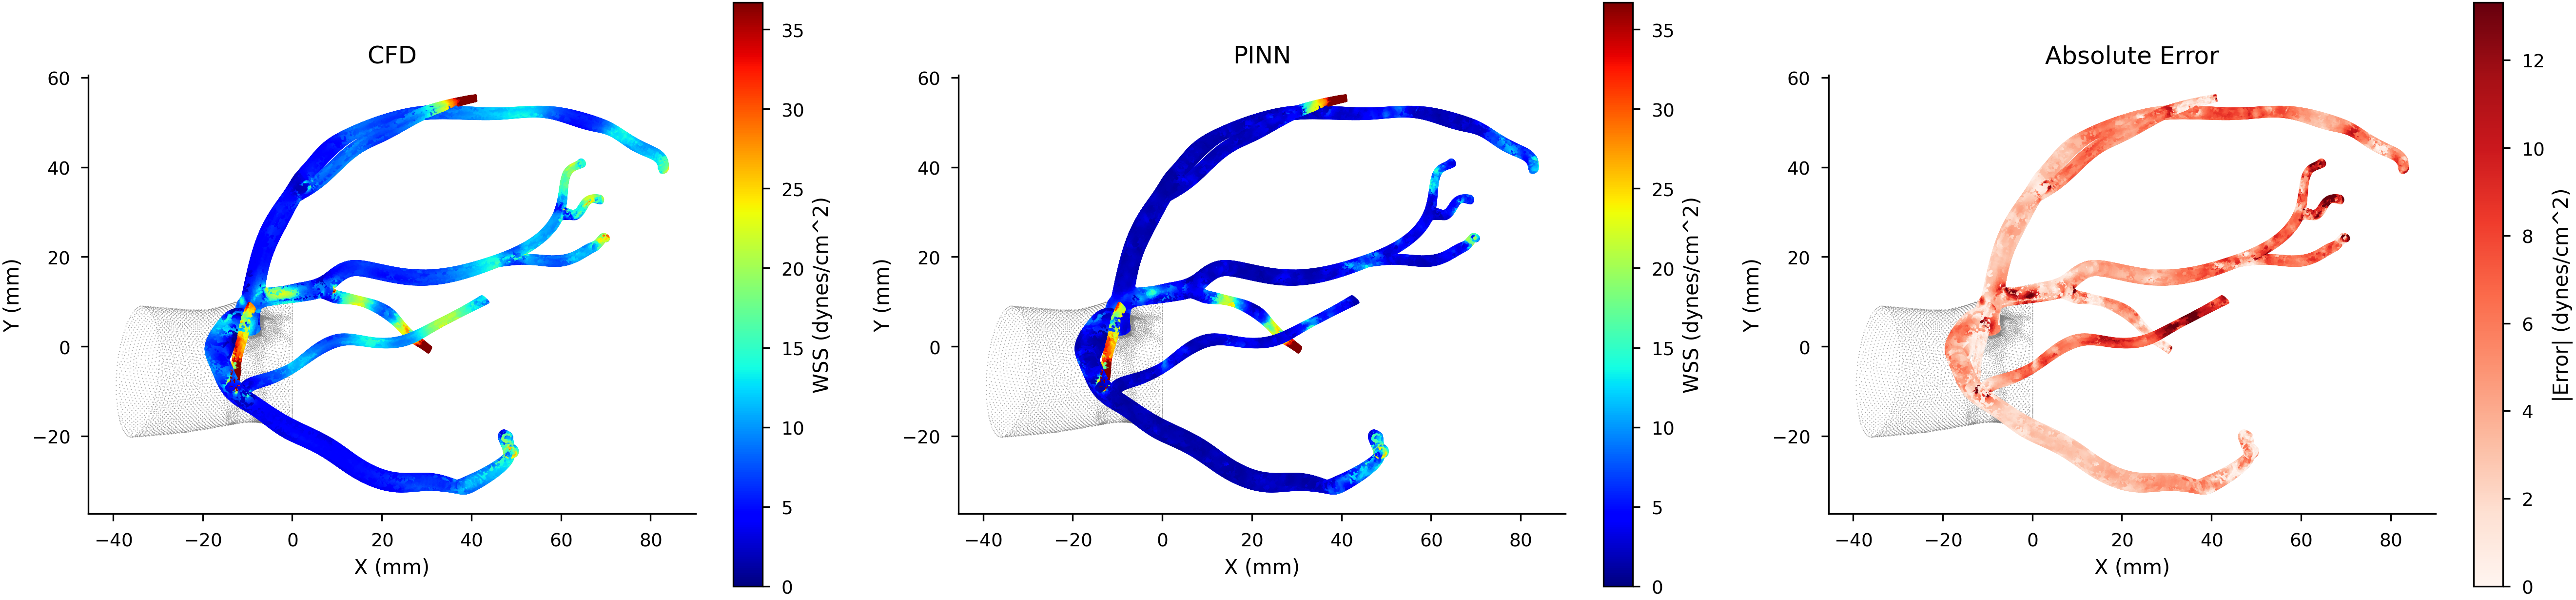
\includegraphics[width=\textwidth]{carreau_yasuda/H1/H1_full_patient_wss_XY.png}
\caption{H1 (Healthy, XY coronal view).}
\label{fig:pinn_wss_h1_cy_xy}
\end{subfigure}\\[4pt]
\begin{subfigure}[t]{\textwidth}
\centering
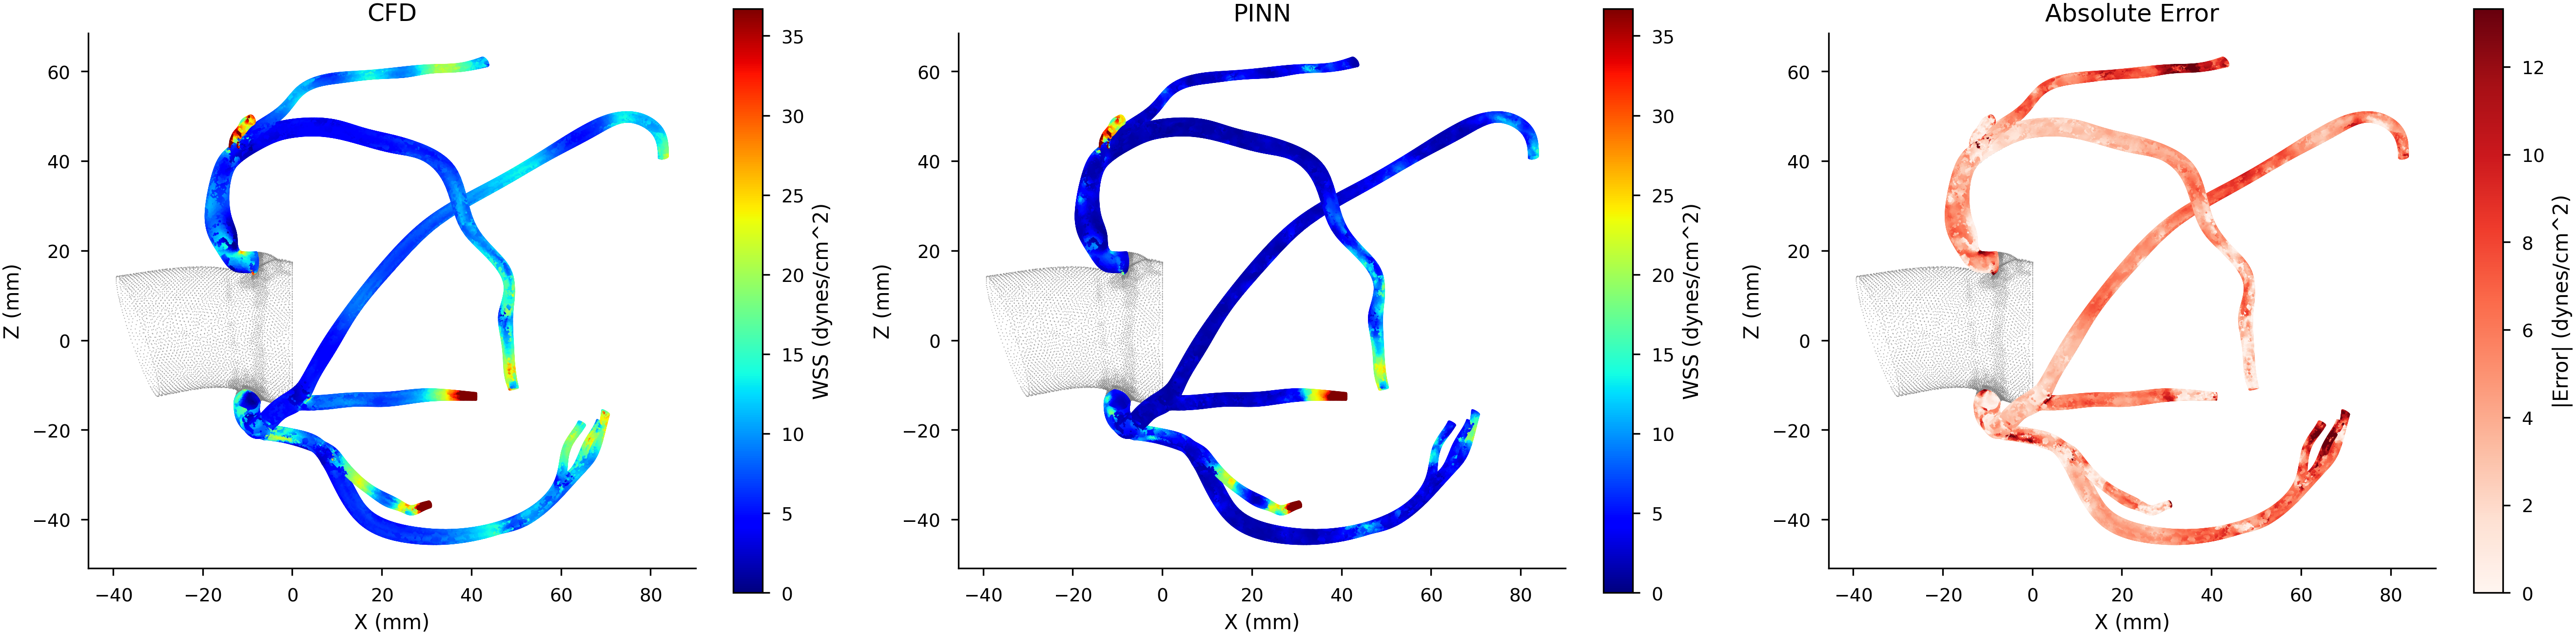
\includegraphics[width=\textwidth]{carreau_yasuda/H1/H1_full_patient_wss_XZ.png}
\caption{H1 (Healthy, XZ sagittal view).}
\label{fig:pinn_wss_h1_cy_xz}
\end{subfigure}
\caption{\addp{Full-patient WSS comparison for the healthy case H1 under the \emph{Carreau--Yasuda} surrogate, shown in the same projections as Figure~\ref{fig:pinn_wss_h1}.}}
\label{fig:pinn_wss_h1_cy}
\end{figure}

\begin{figure}[!htbp]
\centering
\begin{subfigure}[t]{\textwidth}
\centering
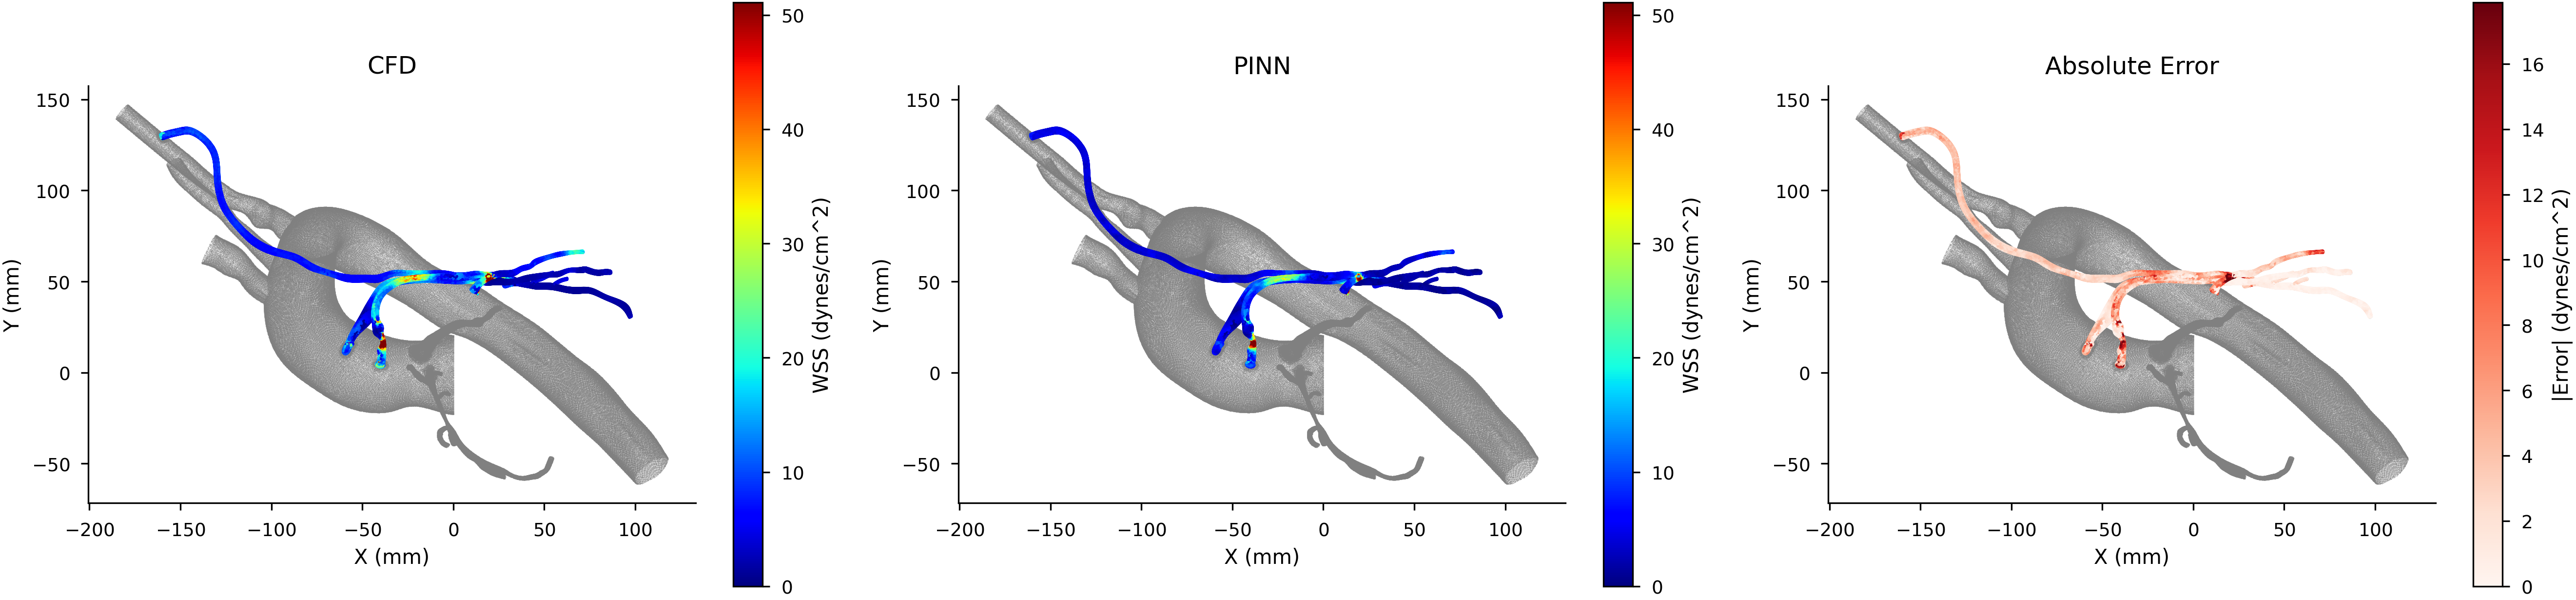
\includegraphics[width=\textwidth]{carreau_yasuda/BG2/BG2_full_patient_wss_XY.png}
\caption{BG2 (SVG, XY coronal view).}
\label{fig:pinn_wss_bg2_cy_xy}
\end{subfigure}\\[4pt]
\begin{subfigure}[t]{\textwidth}
\centering
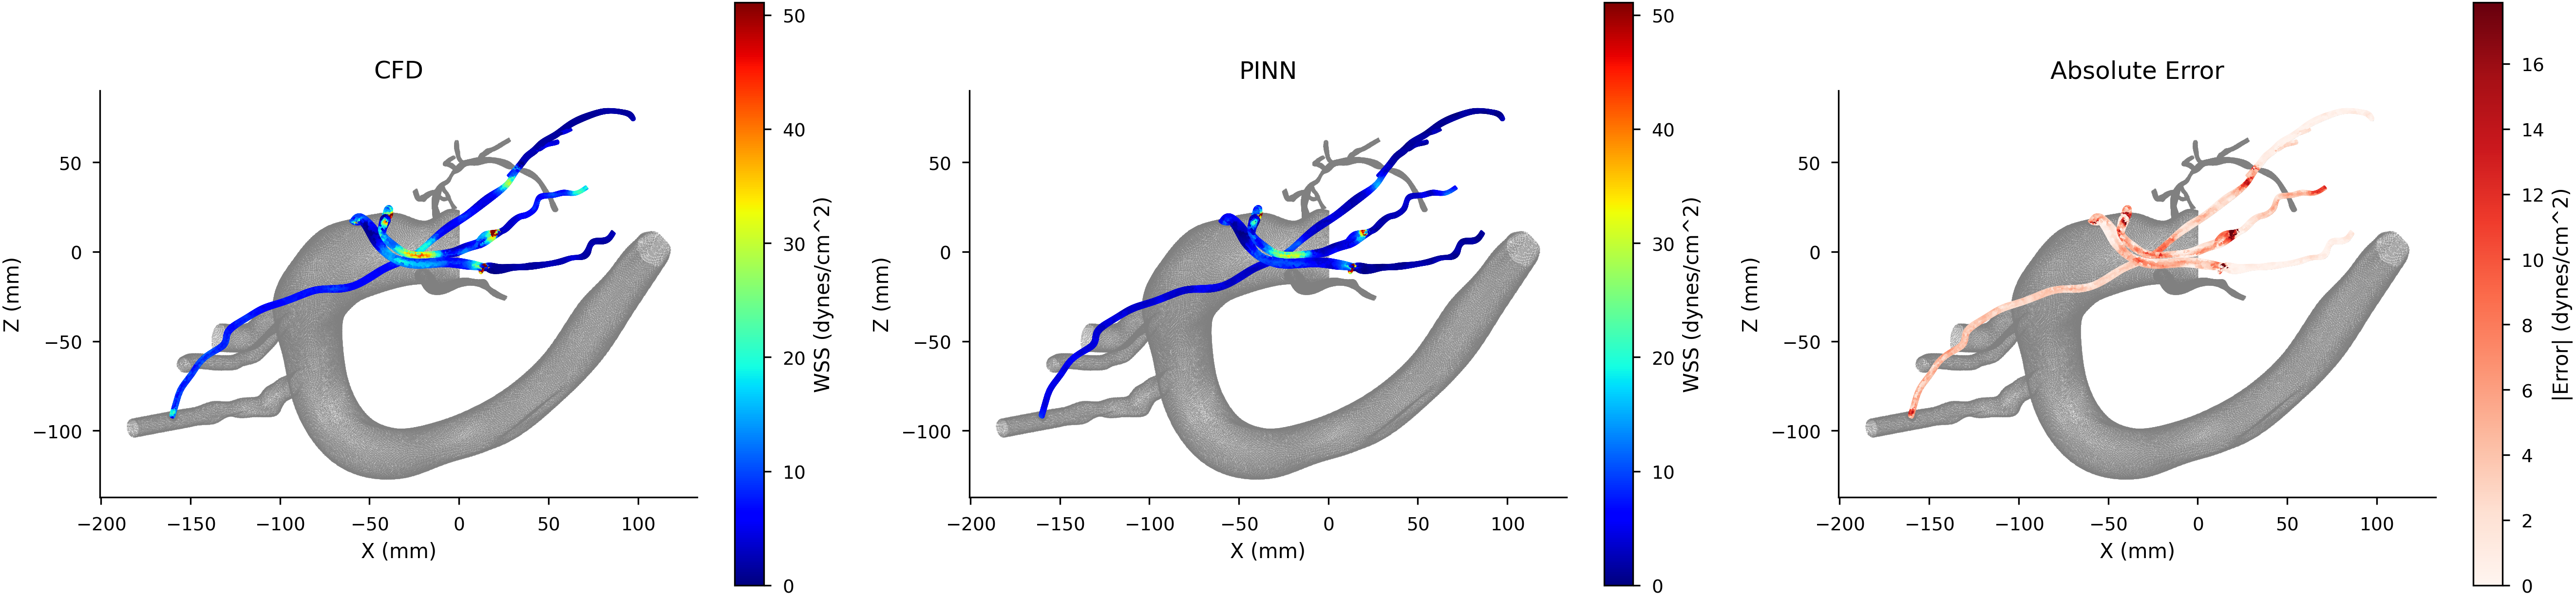
\includegraphics[width=\textwidth]{carreau_yasuda/BG2/BG2_full_patient_wss_XZ.png}
\caption{BG2 (SVG, XZ sagittal view).}
\label{fig:pinn_wss_bg2_cy_xz}
\end{subfigure}\\[4pt]
\begin{subfigure}[t]{\textwidth}
\centering
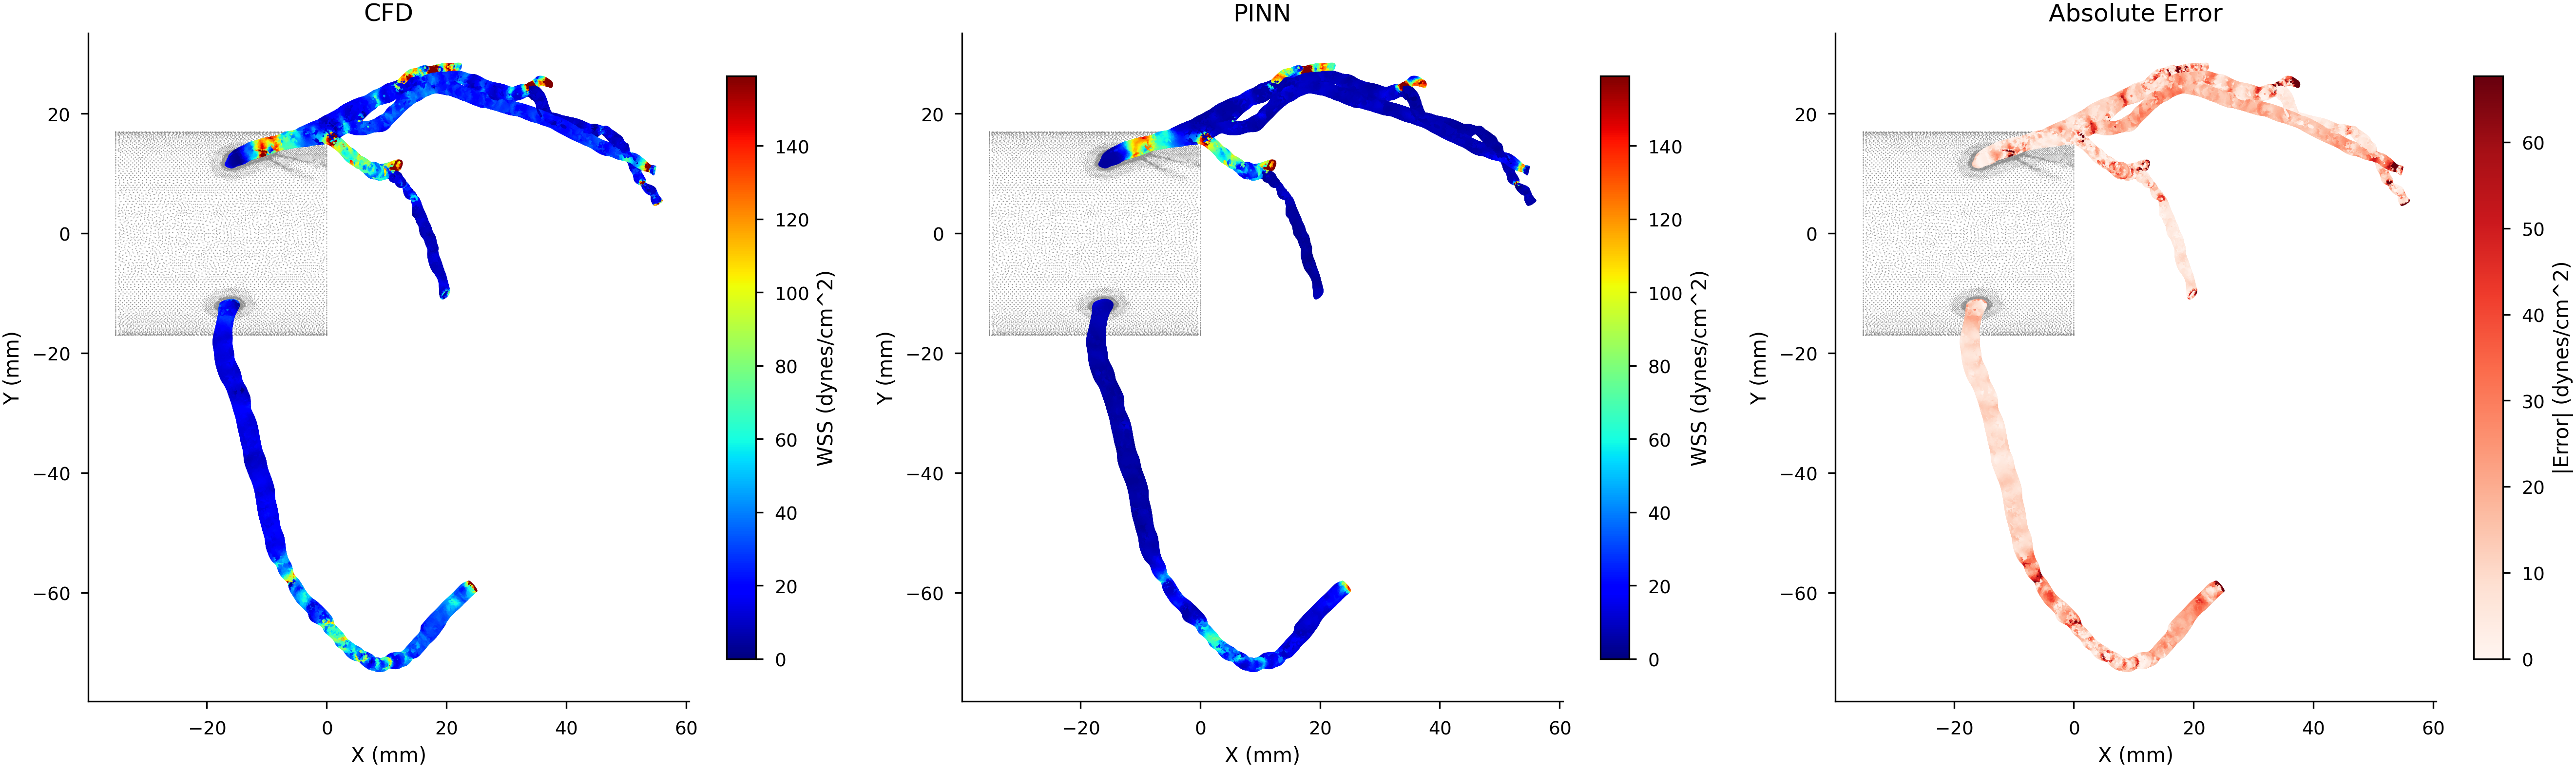
\includegraphics[width=\textwidth]{carreau_yasuda/D3/D3_full_patient_wss_XY.png}
\caption{D3 (Diseased, XY coronal view).}
\label{fig:pinn_wss_d3_cy_xy}
\end{subfigure}\\[4pt]
\begin{subfigure}[t]{\textwidth}
\centering
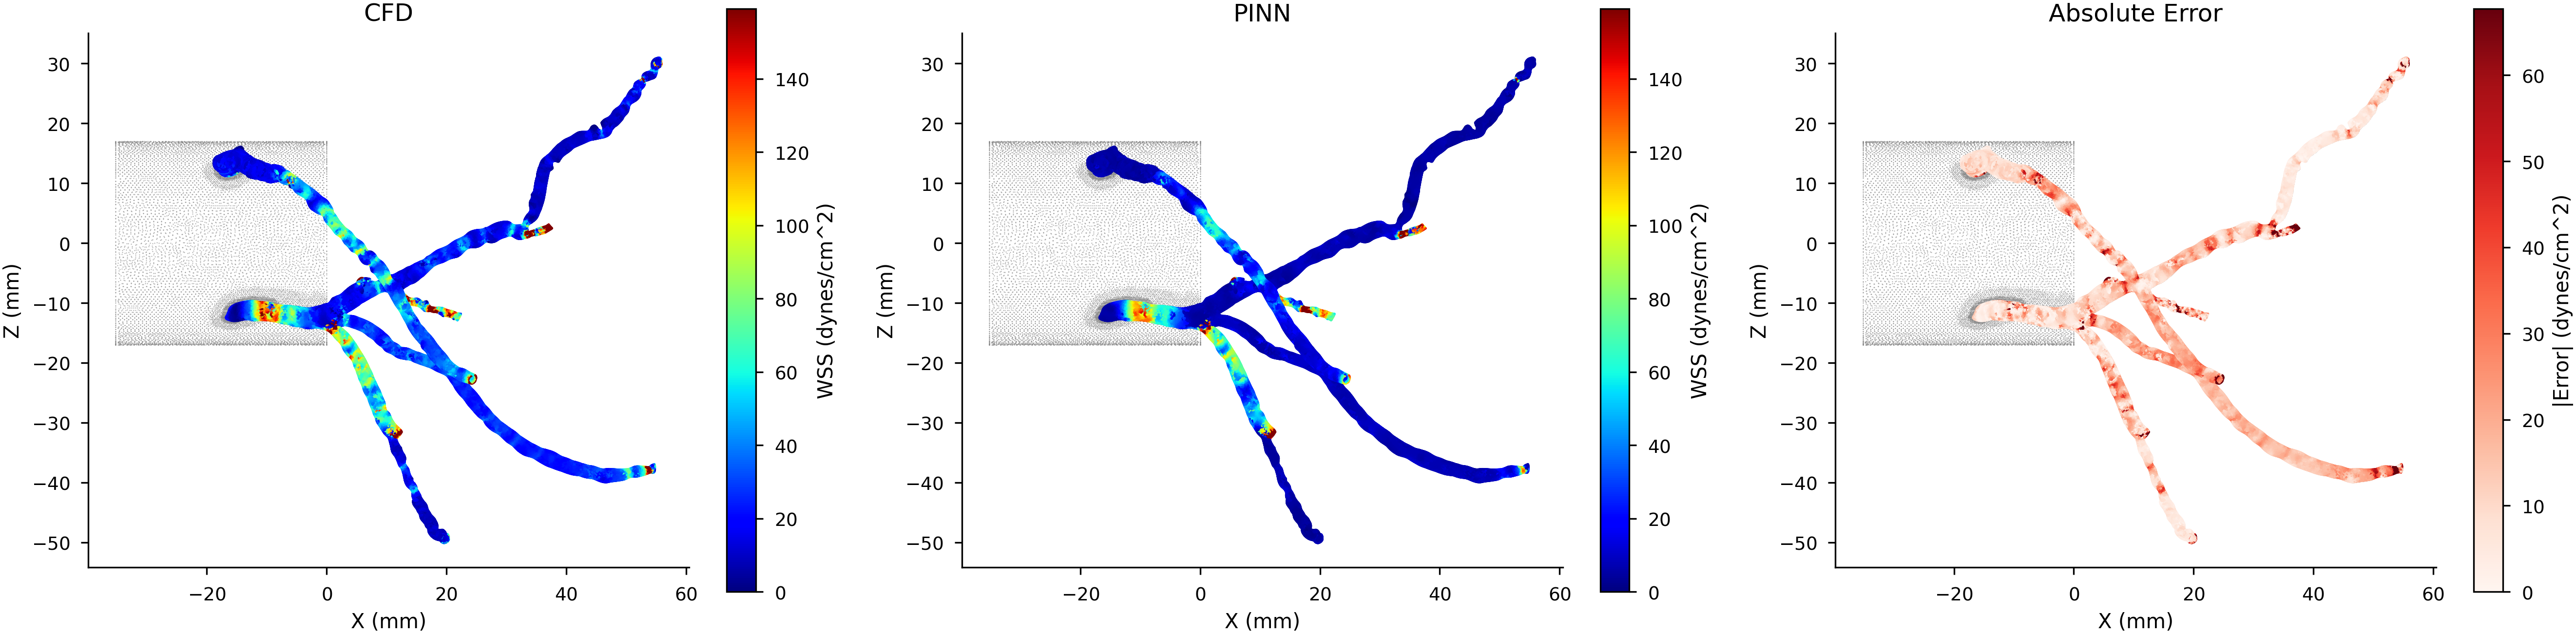
\includegraphics[width=\textwidth]{carreau_yasuda/D3/D3_full_patient_wss_XZ.png}
\caption{D3 (Diseased, XZ sagittal view).}
\label{fig:pinn_wss_d3_cy_xz}
\end{subfigure}
\caption{\addp{Full-patient WSS comparison under the \emph{Carreau--Yasuda} surrogate for the SVG case BG2 (panels a, b) and the diseased case D3 (panels c, d), shown in the same projections as Figure~\ref{fig:pinn_wss_svg_diseased}.}}
\label{fig:pinn_wss_svg_diseased_cy}
\end{figure}

\begin{figure}[htbp]
\centering
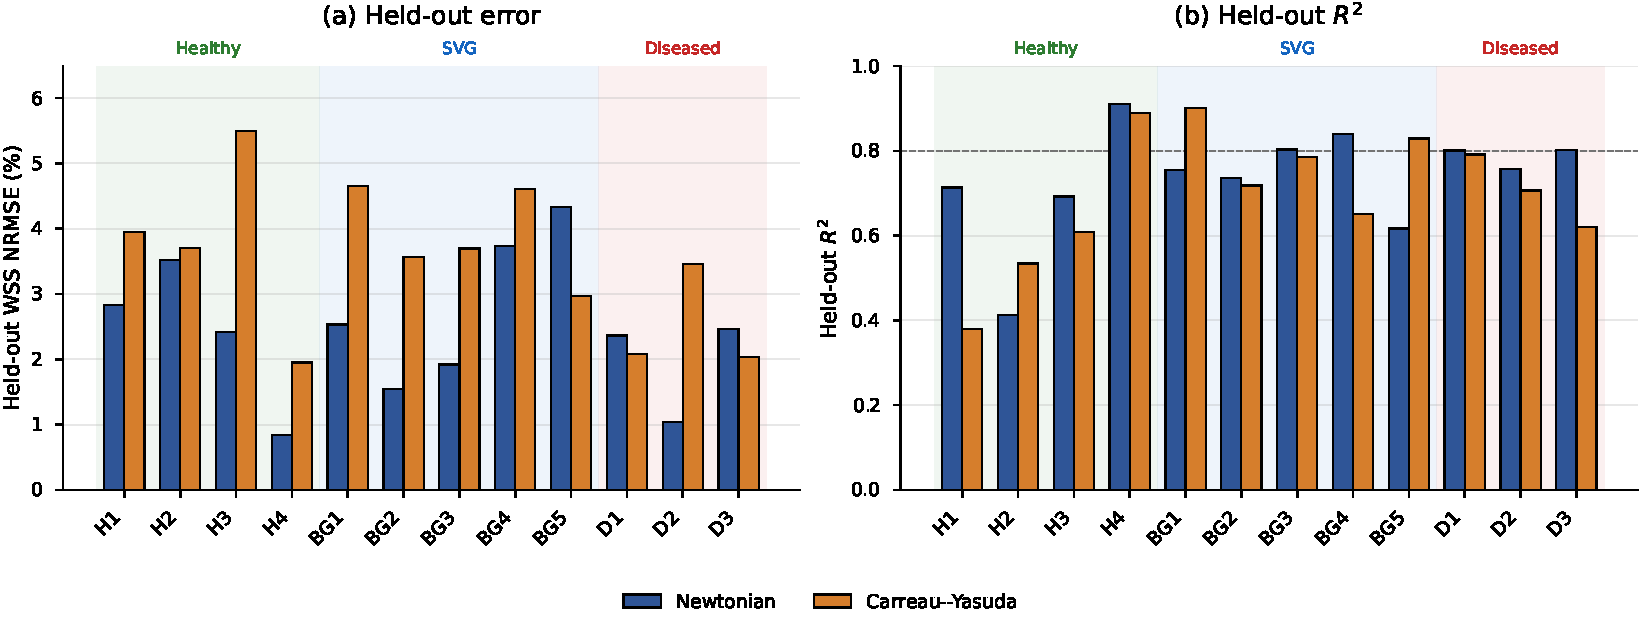
\includegraphics[width=\textwidth]{pinn_holdout_comparison.pdf}
\caption{\textcolor{red}{Per-patient PINN performance under a 20\% spatial holdout for both rheology-matched surrogates. Panel (a) compares held-out WSS NRMSE, and panel (b) compares held-out $R^2$; exact train and holdout values are reported in Tables~\ref{tab:pinn_holdout} and~\ref{tab:pinn_holdout_cy}.}}
\label{fig:pinn_holdout_summary}
\end{figure}

\addp{\subsubsection*{Sensitivity to PINN hyperparameters}
To verify that the reported PINN performance is robust to design choices flagged by the reviewers, we performed three short sensitivity sweeps on the representative patient (H4, Newtonian) using a $200$-epoch training budget. The first probes the loss-balancing scheme by sweeping the clinical-priority factor $\rho_{\mathrm{NS}}$ over four orders of magnitude, $\{0.01, 0.1, 1, 10, 100\}$. The second probes the physics-loss collocation density by sweeping the per-iteration count, $n_c\in\{256, 512, 1024, 2048, 4096\}$. The third probes run-to-run reproducibility by re-training under five random seeds, $\{0,1,2,3,4\}$, at the default hyperparameters. Held-out WSS NRMSE values for all three sweeps are summarised in Table~\ref{tab:pinn_sensitivity}.}

\addp{Across the four orders of magnitude probed for $\rho_{\mathrm{NS}}$, the held-out NRMSE varies between $1.32\%$ and $2.08\%$, a range of $0.76$ percentage points; within $\pm$one order of magnitude of the gradient-norm-balanced default the variation is only $0.36$ percentage points. The collocation sweep shows monotonic improvement with diminishing returns: NRMSE decreases by only $0.10$ percentage points when the count is doubled from $2{,}048$ to $4{,}096$, justifying the production setting. The seed sweep gives a held-out NRMSE of $1.35 \pm 0.17\%$ across five seeds (range $1.14\%$ to $1.55\%$), confirming run-to-run reproducibility. Together these results show that the surrogate's accuracy on held-out points is set primarily by the data and the architecture, and is robust to the specific values of the loss-balancing and collocation hyperparameters.}

\begin{table}[!htbp]
\color{red}
\centering
\setlength{\tabcolsep}{4pt}
\renewcommand{\arraystretch}{0.95}
\caption{\textcolor{red}{PINN sensitivity sweeps on the representative patient (H4, Newtonian) under a $200$-epoch training budget. Each row reports the held-out WSS NRMSE on the same $20\%$ spatial-holdout subset used in Table~\ref{tab:pinn_holdout}.}}
\label{tab:pinn_sensitivity}
\begin{tabular}{|l|c|c|}
\hline
\textbf{Sweep} & \textbf{Setting} & \textbf{Held-out NRMSE (\%)} \\
\hline
\multirow{5}{*}{Loss-weight ($\rho_{\mathrm{NS}}$)}
 & 0.01  & 1.32 \\
 & 0.1   & 1.45 \\
 & 1.0 (default) & 1.55 \\
 & 10.0  & 1.81 \\
 & 100.0 & 2.08 \\
\hline
\multirow{5}{*}{Collocation count $n_c$}
 & 256   & 1.75 \\
 & 512   & 1.68 \\
 & 1024  & 1.65 \\
 & 2048  & 1.60 \\
 & 4096 (default) & 1.55 \\
\hline
\multirow{5}{*}{Random seed}
 & 0 & 1.55 \\
 & 1 & 1.22 \\
 & 2 & 1.48 \\
 & 3 & 1.14 \\
 & 4 & 1.37 \\
\hline
Seed summary & Mean $\pm$ s.d. & $1.35 \pm 0.17$ \\
\hline
\end{tabular}
\end{table}


\section{\label{Clinical Relevance and Limitations}Clinical Relevance and Limitations} 
\hspace*{\parindent}The clinical relevance of this study lies in its ability to simulate and analyze the behavior of WSS in healthy and problematic coronary arteries and grafts, making cross-comparisons between native arteries and SVGs and not limiting the analyses to the primary stenotic regions but trying to find the heterogenous nature of hot-spots with high-WSS that can characterize arteries affected by CAD. It should be remembered that the majority of acute coronary syndromes and myocardial infarctions result from thrombosis and/or embolization due to rupture of the fibrous cap of a nonobstructive coronary plaque \cite{43}. Because WSS is a key factor in the progression of atherosclerosis, plaque formation, and thrombosis, by identifying regions of elevated WSS, clinicians can better predict the plaque zones of high-risk for rupture and acute thrombosis in native coronary arteries and grafts, improving the prognosis of patients undergoing CABG. 

As CFD technology advances and becomes more accessible, it may provide valuable insights into graft performance and facilitate early detection of potential issues, ultimately leading to improved patient outcomes. CFD can potentially become  a valuable tool for both preoperative planning and postoperative monitoring of grafts. Identifying these regions can guide clinical decision-making, leading to more targeted interventions such as stenting or optimized graft placement to reduce the risk of complications. Li et al. \cite{1} presented a universal deep learning technique to predict hemodynamic parameters, comparing its outcomes with CFD. The deep learning model accurately predicted pressure fields for coronary arteries and grafts, effectively replicating pressure distributions and velocity fields in cardiovascular models. The results closely matched CFD and provided reliable clinical indicators for CABG surgery. Sankaran et al. \cite{2} investigated the impact of bypass grafts shape on haemodynamic parameters such as WSS and local velocities in the aorta. They discovered that an anastomosis angle of 70$^0$ best serves the patient's haemodynamics. Their computational tools suggest that individualized surgical geometry could improve the lifespan of grafts. Frauenfelder et al. \cite{5} employed CFD analysis to study how patient-specific geometries in side-to-side and end-to-side anastomoses influence perianastomotic hemodynamics. Their study revealed significant spatial variations in WSS, with side-to-side anastomoses exhibiting more stable hemodynamics and fewer stagnation zones, while end-to-side anastomoses were associated with higher WSS. Nordgaard et al. \cite{6} employed computational fluid dynamics in a swine coronary artery bypass model to examine the effect of competitive flow on WSS in left internal mammary artery (LIMA) grafts. Their findings indicated a negative correlation between high competitive flow and WSS, with high levels leading to low and oscillatory WSS that could cause endothelial dysfunction and graft failure. Conversely, partial competitive flow showed WSS values similar to the ideal no competitive flow condition, suggesting it might be more beneficial. Our results can be interpreted as a guide to focus the future research on assessment of plaque vulnerability in CAD and SVG disease, and we suggest that the assessment should not be limited to the plaques with highest level of stenosis but should also include the bifurcations and also other high-WSS zones determined by the arterial geometry.

{From a clinical translation perspective, the development of PINN-based surrogate models may help address some of the practical barriers that have hindered wider adoption of CFD in cardiovascular care. At present, high-fidelity CFD simulations require access to high-performance computing clusters, commercial software licenses, and considerable computational time resources that are typically available only at specialized research institutions and large academic medical centres. By contrast, a trained PINN model can produce patient-specific WSS predictions within seconds on a standard clinical workstation, potentially bringing hemodynamic biomarkers within reach of community hospitals and outpatient cardiology practices. Looking further ahead, the near-instantaneous inference time of these surrogate models opens intriguing possibilities for intraoperative decision support, where a surgeon might rapidly evaluate alternative graft configurations or stent placements and their likely hemodynamic consequences during the procedure itself. While considerable validation work remains before such applications become clinical reality, these results represent a step toward making patient-specific hemodynamic analysis more accessible.}

While this study provides valuable insights into coronary artery hemodynamics, several limitations must be acknowledged. First, the boundary conditions assume a uniform inlet velocity and zero pressure at the outlet, which may not fully replicate the complex pulsatile flow typically observed in coronary arteries. Blood flow to the coronary arteries primarily occurs during diastolic phase \cite{70, 71}. In clinical scenarios, blood flow is inherently pulsatile, with varying velocities and pressures that influence shear stress dynamics throughout the cardiac cycle. Regarding the pulsatile flow, we neglect this by choice, so that we can maintain the flow rate in the coronary arteries, but it can be done. Future studies incorporating pulsatile flow conditions could provide a more comprehensive understanding of WSS distribution. Second, the no-slip boundary condition used in the simulations neglects the interaction between the blood flow and the vessel walls, which would be captured more accurately by using fluid-structure interaction (FSI) models. FSI models account for the mechanical properties of vessel walls and their deformation under flow-induced forces, providing a more realistic simulation of coronary artery behavior. Lastly, the exclusion of particulate components of blood, such as red blood cells, may underestimate the complexity of blood flow, particularly in regions of high shear. Third, it should be noted that the simplified stenosis model was adopted. Nevertheless, the topic of the present paper is to exhibit the difference between Newtonian and non-Newtonian models. So, this kind of geometry is not idealized and can be regarded as patient-specific to show discrepancy in results. In future study, it is planned to use FSI blood flow model in more complex patient-specific geometry with unsteady boundary conditions. 

About 3 to 5 percent of the total cardiac output reaches coronary arteries, with actual level being higher diastolic phase as noted above. In our work, we assumed that the graft flow is identical to the coronary arteries and distributed the flow accordingly. This may not be the real case in CABG patients and the presence of prior infarcts or collateral remodelling can influence the flow distribution and can be different from healthy controls. Accurately setting flow rates in coronary artery bypass grafts (CABGs) is crucial for studying hemodynamic factors. The literature presents various approaches for defining inlet and outlet conditions in CABG simulations. Some studies employ velocity inlet conditions to model the blood flow entering the graft, while others use mass flow rates to represent the amount of blood supplied. Similarly, at the outlet, boundary conditions may include pressure-based or mass flow rate-based approaches. These variations highlight the complexity and importance of selecting appropriate boundary conditions to ensure realistic simulations and accurate analysis of hemodynamics within CABGs. For instance, Dehlaghi et al. \cite{12} used fully developed inlet boundary conditions and zero pressure outlet boundary conditions with rigid walls and no-slip conditions on the artery walls while studying the effects of stent geometry on blood flow in stented human coronary arteries using 2D and 3D CFD models. Other studies employed a lumped parameter heart model at the inlet and a lumped parameter coronary vascular model at the outlets, with a three-element Windkessel model applied to the descending thoracic aorta \cite{13, 14, 18}. Tran et al. \cite{15, 17} applied pulsatile flow inlet boundary conditions and set resistance and capacitance boundary conditions at the outlets. Koyama et al. \cite{16} used flow rate inlet boundary conditions and peripheral impedance at the outlet boundary conditions. Additionally, Mohammadi et al. \cite{19} compared velocity-based and pressure-based boundary conditions in CFD simulations of stenosed coronary arteries, finding that both methods yield similar flow rates and velocities up to a 10\% diameter reduction. In our study, we utilized a range of boundary conditions, including uniform velocity at the inlet and pressure or mass flow outlets, to achieve the target flow in the coronary arteries. These varied methodologies highlight the importance of selecting appropriate boundary conditions to accurately capture the physiological characteristics and flow dynamics in CABG simulations. Proper consideration of boundary conditions is crucial for replicating the realistic hemodynamic environment, thus improving the predictive accuracy of CFD models for surgical planning and evaluation. 

Because CFD results are mainly shaped by the vessel geometry, accurate 3D reconstruction of the coronary artery lumen is essential for the accuracy of the results \cite{75}. CT angiograms can introduce artifacts or incorrectly image complex 3D geometry, particularly at bifurcations \cite{76, 77}. This study was based on  repositories that were prepared for prior studies but then were made available either publicly or upon request. While we are limited by the accuracy of the prior sources, the high spatial resolution and detail of the 3D models that were used in this study, and the fact that whole aortic arch and coronary branches were included in the models especially for the Vascular Model Datasets increases the strength of our study.

Finally, we did not associate CFD simulation results with underlying geometric measurement. Future work on better characterization of the vascular structure features that lead to high WSS zones, can be beneficial for understanding the nature of WSS changes in CAD and SVG disease.

\addp{The PINN surrogate has its own caveats, distinct from those of the underlying CFD. Most importantly, each trained model is specific to a single patient geometry. The reported per-patient accuracy therefore quantifies how well the surrogate reproduces CFD on the same vasculature it was trained on. It does not measure generalisation across patients. Applying the approach to a new patient requires a fresh training run, with the per-patient wall-clock cost reported below. Cross-patient generalisation, for example via transfer learning from a pre-trained backbone or a multi-patient encoder shared across geometries, is a natural extension and is left for future work.}

\addp{PINN training takes between $5$ and $55$~min per patient on a single mid-range GPU. The trained surrogate then predicts a full 3D WSS field in under one second, several orders of magnitude faster than re-running a fresh CFD simulation on the same geometry. The dominant cost in the end-to-end clinical workflow is therefore not the surrogate itself but the upstream image-segmentation and meshing pipeline, which is shared with the CFD route and is unaffected by the choice of solver. The surrogate becomes most attractive when many predictions per patient are needed --- for example to evaluate alternative graft configurations or to support intraoperative decision making --- because the one-off training cost is then amortised across many inferences.}

\addp{Three further caveats follow from the way the surrogate is supervised. First, because the PINN learns from CFD data, the fidelity of its predictions is fundamentally tied to the quality of the underlying simulations, and any modelling assumptions or numerical errors present in the CFD solution carry through to the surrogate. Second, the implementation is restricted to steady-state conditions, matching the CFD simulations performed here; extending the framework to pulsatile, time-varying flow would require substantial changes to the network architecture and substantially larger training datasets. Third, the held-out errors reported in Tables~\ref{tab:pinn_holdout} and~\ref{tab:pinn_holdout_cy} are aggregated over each patient's full mesh. The per-patient WSS contour comparisons (Figures~\ref{fig:pinn_wss_h1}--\ref{fig:pinn_wss_svg_diseased_cy}) qualitatively show that the largest pointwise residuals concentrate at high-curvature regions and at the immediate neighbourhoods of bifurcations, anastomoses and stenoses, where wall-normal velocity gradients are steepest. A formal near-wall versus core decomposition with bounding-box-tagged stenosis and bifurcation regions is the natural next step and is left for future work. Outside the conditions seen during training, the surrogate's predictions should be treated with caution, as neural networks generally extrapolate poorly.}

Despite these limitations, this study offers valuable insights into the hemodynamics of coronary arteries and grafts, providing a foundation for future research to improve clinical outcomes in CAD. Incorporating more sophisticated models, including FSI and pulsatile flow, could yield more clinically applicable results. 

\section{\label{Conclusion}Conclusion} 
\hspace*{\parindent} 
This study highlights the critical role of WSS in identifying diseased regions in coronary arteries and SVGs used in CABG surgery, {combining traditional CFD analysis with physics-informed machine learning}. By employing both Newtonian and Carreau-Yasuda models, our findings reinforce the clinical relevance of WSS thresholds in detecting high-risk areas linked to cardiovascular disease progression. Our analysis from the five computed parameters reveals that areas exceeding 40 dynes/cm$^2$ may indicate diseased conditions resulting from stenosis, abnormal curvatures, tortuosity, or problematic bifurcations with high-risk plaques. While 3D WSS contours showed little visible difference between healthy and diseased vessels, statistical analysis provided clearer distinctions, with the Carreau–Yasuda model demonstrating higher sensitivity than the Newtonian model in detecting elevated WSS. Conversely, regions below this threshold are deemed healthy. 

{We created PINN surrogate models that forecast WSS distributions while satisfying the incompressible Navier--Stokes equations as soft physics constraints, with the aim of lowering the computational cost of recurrent CFD simulations. \addp{The surrogates were trained on twelve patient cases spanning healthy, diseased, and SVG categories using rheology-matched physics losses against both Newtonian and Carreau--Yasuda CFD. On a 20\% spatial holdout, the Newtonian surrogate reached a mean NRMSE of 2.46\% and $R^2 = 0.74$. The Carreau--Yasuda surrogate reached 3.52\% and $R^2 = 0.70$ on the same protocol. The held-out Pearson correlation was $r = 0.93$ under both rheologies. These results demonstrate that physics-informed neural networks can accurately reproduce CFD results for coronary hemodynamic analysis.} \replaced[id=pinn]{Once trained, each PINN model predicts a full 3D WSS field in under one second on the same hardware, several orders of magnitude faster than re-running CFD on the same geometry.}{Once trained, each PINN model can predict full 3D WSS fields in seconds compared to the hours required for traditional CFD simulations.}}

These results underscore the value of advanced CFD modeling {in combination with physics-informed surrogate models} for improving patient outcomes and guiding personalized treatment strategies.

\section*{Conflicts of Interest}
The authors have no conflicts to disclose.

\section*{Author Contribution}{Author Contributions: Conceptualization, M.A.U.R. (Muhammad Abaid Ur Rehman), Ö.E. (Özgür Ekici), Ş.E.E. (Şefik Evren Erdener), M.A.O. (Michael Ajao-Olarinoye) and {A.G.K. (Alex G. Kuchumov)}; methodology, M.A.U.R., Ö.E. {and M.A.O.}; software, M.A.U.R., Ö.E. {and M.A.O.}; validation, M.A.U.R., Ö.E., Ş.E.E., {M.A.O.} and  F.J. (Fei Jia); formal analysis, M.A.U.R., Ö.E., Ş.E.E., { M.A.O.} and F.J.; investigation, M.A.U.R., Ö.E. and Ş.E.E.; resources, M.A.U.R., Ö.E. and Ş.E.E.; data curation, M.A.U.R., Ö.E. and Ş.E.E.; writing original draft preparation, M.A.U.R., A.G.K., Ş.E.E. {and M.A.O.}; writing review and editing, M.A.U.R., Ö.E., Ş.E.E. {and M.A.O.}; visualization, M.A.U.R., Ö.E., Ş.E.E., {M.A.O.} and  F.J. ; supervision, Ö.E. and Ş.E.E.; {physics-informed neural network development and implementation, M.A.O.} All authors have read and agreed to the published version of the manuscript.}

\section*{Data Availability}{The data generated in this study can be made available by corresponding author following a request. {The PyTorch codes and CFD training data used to generate the PINN results in the manuscript are publicly available on GitHub at \url{https://github.com/michaelajao/CABG_WSS_PINN}.}}

\section*{Compliance with Ethical Standards}

\subsection*{Disclosure of Potential Conflicts of Interest}
The authors declare that they have no conflict of interest.

\subsection*{Research Involving Human Participants and/or Animals}
This research utilizes open-source models related to Coronary Artery Bypass Grafting (CABG) from the \url{www.vascularmodel.org} website and ASOCA. All models are publicly available and do not involve direct research with human participants or animals.

\subsection*{Informed Consent}
Informed consent was not applicable as this study did not involve human participants.


\newpage
\clearpage
		
\begin{thebibliography}{}
\bibitem{1} Li, G., Wang, H., Zhang, M., Tupin, S., Qiao, A., Liu, Y., ... \& Anzai, H. (2021). Prediction of 3D Cardiovascular hemodynamics before and after coronary artery bypass surgery via deep learning. Communications biology, 4(1), 99. \url{https://doi.org/10.1038/s42003-020-01638-1}

\bibitem{2} ankaran, S., Esmaily Moghadam, M., Kahn, A. M., Tseng, E. E., Guccione, J. M., \& Marsden, A. L. (2012). Patient-specific multiscale modeling of blood flow for coronary artery bypass graft surgery. Annals of biomedical engineering, 40, 2228-2242. \url{https://doi.org/10.1007/s10439-012-0579-3} 

\bibitem{3} Khan, M. O., Tran, J. S., Zhu, H., Boyd, J., Packard, R. R. S., Karlsberg, R. P., ... \& Marsden, A. L. (2021). Low wall shear stress is associated with saphenous vein graft stenosis in patients with coronary artery bypass grafting. Journal of cardiovascular translational research, 14, 770-781. \url{https://doi.org/10.1007/s12265-020-09982-7}

\bibitem{4} Mehta, D., Izzat, M. B., Bryan, A. J., \& Angelini, G. D. (1997). Towards the prevention of vein graft failure. International journal of cardiology, 62, S55-S63.
\url{https://doi.org/10.1016/S0167-5273(97)00214-3}

\bibitem{5} Frauenfelder, T., Boutsianis, E., Schertler, T., Husmann, L., Leschka, S., Poulikakos, D., ... \& Alkadhi, H. (2007). Flow and wall shear stress in end-to-side and side-to-side anastomosis of venous coronary artery bypass grafts. Biomedical engineering online, 6, 1-13. \url{https://doi.org/10.1186/1475-925X-6-35} 

\bibitem{6} Nordgaard, H., Swillens, A., Nordhaug, D., Kirkeby-Garstad, I., Van Loo, D., Vitale, N., ... \& Lovstakken, L. (2010). Impact of competitive flow on wall shear stress in coronary surgery: computational fluid dynamics of a LIMA–LAD model. Cardiovascular Research, 88(3), 512-519. \url{https://doi.org/10.1093/cvr/cvq210}

\bibitem{7} Sandeep, S., \& Shine, S. R. (2021). Effect of stenosis and dilatation on the hemodynamic parameters associated with left coronary artery. Computer Methods and Programs in Biomedicine, 204, 106052. \url{https://doi.org/10.1016/j.cmpb.2021.106052}

\bibitem{8} Xu, K., Yu, L., Wan, J., Wang, S., \& Lu, H. (2020). The influence of the elastic modulus of the plaque in carotid artery on the computed results of FFRCT. Computer Methods in Biomechanics and Biomedical Engineering, 23(5), 201-211. \url{https://doi.org/10.1080/10255842.2019.1710741}

\bibitem{9} Johnston, B. M., Johnston, P. R., Corney, S., \& Kilpatrick, D. (2004). Non-Newtonian blood flow in human right coronary arteries: steady state simulations. Journal of biomechanics, 37(5), 709-720. \url{https://doi.org/10.1016/j.jbiomech.2003.09.016}

\bibitem{10} Johnston, B. M., Johnston, P. R., Corney, S., \& Kilpatrick, D. (2006). Non-Newtonian blood flow in human right coronary arteries: transient simulations. Journal of biomechanics, 39(6), 1116-1128. \url{https://doi.org/10.1016/j.jbiomech.2005.01.034}

\bibitem{11} Dur, O., Coskun, S. T., Coskun, K. O., Frakes, D., Kara, L. B., \& Pekkan, K. (2011). Computer-aided patient-specific coronary artery graft design improvements using CFD coupled shape optimizer. Cardiovascular engineering and technology, 2, 35-47. \url{https://doi.org/10.1007/s13239-010-0029-z}

\bibitem{12} Dehlaghi, V., Shadpoor, M. T., \& Najarian, S. (2008). Analysis of wall shear stress in stented coronary artery using 3D computational fluid dynamics modeling. Journal of materials processing technology, 197(1-3), 174-181. \url{https://doi.org/10.1016/j.jmatprotec.2007.06.010}

\bibitem{13} Kim, H. J., Vignon-Clementel, I. E., Coogan, J. S., Figueroa, C. A., Jansen, K. E., \& Taylor, C. A. (2010). Patient-specific modeling of blood flow and pressure in human coronary arteries. Annals of biomedical engineering, 38, 3195-3209. \url{https://doi.org/10.1007/s10439-010-0083-6}

\bibitem{14} Rezaeimoghaddam, M., Oguz, G. N., Ates, M. S., Bozkaya, T. A., Piskin, S., Samaneh Lashkarinia, S., ... \& Pekkan, K. (2020). Patient-specific hemodynamics of new coronary artery bypass configurations. Cardiovascular Engineering and Technology, 11, 663-678. \url{https://doi.org/10.1007/s13239-020-00493-9}

\bibitem{15} Tran-Nguyen, N., Yan, A. T., Fremes, S., Triverio, P., \& Jimenez-Juan, L. (2023). Abnormal wall shear stress area is correlated to coronary artery bypass graft remodeling 1 year after surgery. Annals of Biomedical Engineering, 51(7), 1588-1601. \url{https://doi.org/10.1007/s10439-023-03167-4}

\bibitem{16} Koyama, S., Kitamura, T., Itatani, K., Yamamoto, T., Miyazaki, S., Oka, N., ... \& Miyaji, K. (2016). Impact of top end anastomosis design on patency and flow stability in coronary artery bypass grafting. Heart and vessels, 31, 643-648. \url{https://doi.org/10.1007/s00380-015-0680-2}

\bibitem{17} Tran-Nguyen, N., Condemi, F., Yan, A., Fremes, S., Triverio, P., \& Jimenez-Juan, L. (2022). Wall shear stress differences between arterial and venous coronary artery bypass grafts one month after surgery. Annals of Biomedical Engineering, 50(12), 1882-1894. \url{https://doi.org/10.1007/s10439-022-03007-x}

\bibitem{18} Seo, J., Ramachandra, A. B., Boyd, J., Marsden, A. L., \& Kahn, A. M. (2022, June). Computational evaluation of venous graft geometries in coronary artery bypass surgery. In Seminars in thoracic and cardiovascular surgery (Vol. 34, No. 2, pp. 521-532). WB Saunders. \url{https://doi.org/10.1053/j.semtcvs.2021.03.007}

\bibitem{19} Mohammadi, H., \& Bahramian, F. (2009). Boundary conditions in simulation of stenosed coronary arteries. Cardiovascular Engineering, 9, 83-91. \url{https://doi.org/10.1007/s10558-009-9078-z}

\bibitem{20} Sankaranarayanan, M., Chua, L. P., Ghista, D. N., \& Tan, Y. S. (2005). Computational model of blood flow in the aorto-coronary bypass graft. Biomedical engineering online, 4, 1-13. \url{https://doi.org/10.1186/1475-925X-4-14}

\bibitem{21} Golshirazi, A. H., \& Javanbakht, V. (2023). Effects of anastomotic angles and distances of the bypass graft to the stenosis on blood flow hydrodynamics in a bypass grafting coronary artery. Journal of Clinical Cardiology, 3(2), 60-70.\url{https://doi.org/10.33696/cardiology.2.036}

\bibitem{22} Thakare, V., Sontakke, N. G., Wasnik Sr, P., \& Kanyal, D. (2023). Recent Advances in Coronary Artery Bypass Grafting Techniques and Outcomes: A Narrative Review. Cureus, 15(9). \url{https://doi.org/10.7759/cureus.45511}

\bibitem{23} Marzoog, B. A., Alexandrovich, K. O., Nikolaevich, T. M., \& Vladimirovich, K. S. (2023). Post-Coronary Artery Bypass Graft Complications; Potential Causes and Risk Factors. MedRxiv, 2022-12. \url{https://doi.org/10.1101/2022.12.29.22284005}

\bibitem{24} Dong, S., Zhao, Z., Huang, X., Ma, M., Yang, Z., Fan, C., ... \& Zhou, Y. (2023). Triglyceride-glucose index is associated with poor prognosis in acute coronary syndrome patients with prior coronary artery bypass grafting undergoing percutaneous coronary intervention. Cardiovascular Diabetology, 22(1), 286. \url{https://doi.org/10.1186/s12933-023-02029-6}

\bibitem{25} Sethi, P. S., Nance, J., Johnson, D., Wilke, J., Wilson, K., Hall, R., ... \& Morrison, D. A. (2003). A comprehensive cardiac rehabilitation program in post-CABG patients: a rationale and critical pathway. Critical Pathways in Cardiology, 2(1), 20-33. \url{https://doi.org/10.1097/01.HPC.0000057391.93352.AA}

\bibitem{26} Berger, S. A., \& Jou, L. D. (2000). Flows in stenotic vessels. Annual review of fluid mechanics, 32(1), 347-382.  \url{https://doi.org/10.1146/annurev.fluid.32.1.347}

\bibitem{27} Pedley, T.J., (1980). The Fluid Mechanics of Large Blood Vessels. Cambridge University Press, Cambridge. \url{https://doi.org/10.1017/cbo9780511896996}

\bibitem{29} Sadeghi, M. R., Jahangiri, M., \& Saghafian, M. (2020). The impact of uniform magnetic field on the pulsatile non-Newtonian blood flow in an elastic stenosed artery. Journal of the Brazilian Society of Mechanical Sciences and Engineering, 42, 1-15. \url{https://doi.org/10.1007/s40430-020-02651-5}  

\bibitem{30} Liu, H., Lan, L., Abrigo, J., Ip, H. L., Soo, Y., \& Zheng, D. (2021). Comparison of Newtonian and non-Newtonian fluid models in blood flow simulation in patients with intracranial arterial stenosis. Front Physiol. 2021; 12: 718540. \url{https://doi.org/10.3389/fphys.2021.718540}

\bibitem{31} Gharleghi, R., Adikari, D., Ellenberger, K., Webster, M., Ellis, C., Sowmya, A., ... \& Beier, S. (2023). Annotated computed tomography coronary angiogram images and associated data of normal and diseased arteries. Scientific Data, 10(1), 128. \url{https://doi.org/10.1038/s41597-023-02016-2}

\bibitem{32} Lynch, S., Nama, N., \& Figueroa, C. A. (2022). Effects of non-Newtonian viscosity on arterial and venous flow and transport. Scientific Reports, 12(1), 20568. \url{https://doi.org/10.1038/s41598-022-19867-1}

\bibitem{33} Shimizu, T., Ito, S., Kikuchi, Y., Misaka, M., Hirayama, T., Ishimaru, S., \& Yamashina, A. (2004). Arterial conduit shear stress following bypass grafting for intermediate coronary artery stenosis: a comparative study with saphenous vein grafts. European journal of cardio-thoracic surgery, 25(4), 578-584. \url{https://doi.org/10.1016/j.ejcts.2003.12.039}

\bibitem{34} World Health Organization. (2021, June 11). \textit{Cardiovascular diseases (CVDs)}. Retrieved from: \url{https://www.who.int/news-room/fact-sheets/detail/cardiovascular-diseases-(cvds)}

\bibitem{35} Velagaleti, R. S., \& Vasan, R. S. (2007). Heart failure in the twenty-first century: is it a coronary artery disease or hypertension problem?. Cardiology clinics, 25(4), 487-495. \url{https://doi.org/10.1016/j.ccl.2007.08.010}

\bibitem{36} Writing Committee Members*, Hillis, L. D., Smith, P. K., Anderson, J. L., Bittl, J. A., Bridges, C. R., ... \& Winniford, M. D. (2011). 2011 ACCF/AHA guideline for coronary artery bypass graft surgery: a report of the American College of Cardiology Foundation/American Heart Association Task Force on Practice Guidelines. Circulation, 124(23), e652-e735. \url{https://doi.org/10.1161/CIR.0b013e31823c074e}

\bibitem{37} Goldman, S., Zadina, K., Moritz, T., Ovitt, T., Sethi, G., Copeland, J. G., \& VA Cooperative Study Group. (2004). Long-term patency of saphenous vein and left internal mammary artery grafts after coronary artery bypass surgery: results from a Department of Veterans Affairs Cooperative Study. Journal of the American College of Cardiology, 44(11), 2149-2156. \url{https://doi.org/10.1016/j.jacc.2004.08.064}

\bibitem{38} Xenogiannis, I., Zenati, M., Bhatt, D. L., Rao, S. V., Rodes-Cabau, J., Goldman, S., ... \& Brilakis, E. S. (2021). Saphenous vein graft failure: from pathophysiology to prevention and treatment strategies. Circulation, 144(9), 728-745. \url{https://doi.org/10.1161/CIRCULATIONAHA.120.052163}

\bibitem{39} Litwinowicz, R., Mazur, P., Śliwiński, P., Bryndza, M., Bartuś, K., Filip, G., ... \& Kędziora, A. (2022). Long-term survival following postoperative myocardial infraction after coronary artery bypass surgery. Journal of Thoracic Disease, 14(1), 102. \url{https://doi.org/10.21037/jtd-21-1279}

\bibitem{40} Kolossváry, M., Szilveszter, B., Merkely, B., \& Maurovich-Horvat, P. (2017). Plaque imaging with CT—a comprehensive review on coronary CT angiography based risk assessment. Cardiovascular diagnosis and therapy, 7(5), 489. \url{https://doi.org/10.21037/cdt.2016.11.06}

\bibitem{41} Chan, K. H., \& Ng, M. K. (2013). Is there a role for coronary angiography in the early detection of the vulnerable plaque?. International journal of cardiology, 164(3), 262-266. \url{https://doi.org/10.1016/j.ijcard.2012.01.027}

\bibitem{42} Sun, Z., \& Xu, L. (2014). Computational fluid dynamics in coronary artery disease. Computerized medical imaging and graphics, 38(8), 651-663. \url{https://doi.org/10.1016/j.compmedimag.2014.09.002}

\bibitem{43} Tobis, J., Azarbal, B., \& Slavin, L. (2007). Assessment of intermediate severity coronary lesions in the catheterization laboratory. Journal of the American College of Cardiology, 49(8), 839-848. \url{https://doi.org/10.1016/j.jacc.2006.10.055}

\bibitem{44} Govindaraju, K., Badruddin, I. A., Viswanathan, G. N., Ramesh, S. V., \& Badarudin, A. (2013). Evaluation of functional severity of coronary artery disease and fluid dynamics' influence on hemodynamic parameters: A review. Physica Medica, 29(3), 225-232. \url{https://doi.org/10.1016/j.ejmp.2012.03.008}

\bibitem{45} Kim, Y. K., Jang, C. W., Kwon, S. H., Kim, J. H., Lerman, A., \& Bae, J. H. (2021). Ten‐year clinical outcomes in patients with intermediate coronary stenosis according to the combined culprit lesion. Clinical Cardiology, 44(8), 1161-1168. \url{https://doi.org/10.1002/clc.23668}

\bibitem{46} Morbiducci, U., Kok, A. M., Kwak, B. R., Stone, P. H., Steinman, D. A., \& Wentzel, J. J. (2016). Atherosclerosis at arterial bifurcations: evidence for the role of haemodynamics and geometry. Thrombosis and haemostasis, 115(03), 484-492. \url{https://doi.org/10.1160/TH15-07-0597}

\bibitem{47} Zhou, M., Yu, Y., Chen, R., Liu, X., Hu, Y., Ma, Z., ... \& Wang, L. (2023). Wall shear stress and its role in atherosclerosis. Frontiers in cardiovascular medicine, 10, 1083547. \url{https://doi.org/10.3389/fcvm.2023.1083547}

\bibitem{49} Kumar, A., Hung, O. Y., Piccinelli, M., Eshtehardi, P., Corban, M. T., Sternheim, D., ... \& Samady, H. (2018). Low coronary wall shear stress is associated with severe endothelial dysfunction in patients with nonobstructive coronary artery disease. JACC: Cardiovascular Interventions, 11(20), 2072-2080. \url{https://doi.org/10.1016/j.jcin.2018.07.004}

\bibitem{50} Stone, P. H., Saito, S., Takahashi, S., Makita, Y., Nakamura, S., Kawasaki, T., ... \& Feldman, C. L. (2012). Prediction of progression of coronary artery disease and clinical outcomes using vascular profiling of endothelial shear stress and arterial plaque characteristics: the PREDICTION Study. Circulation, 126(2), 172-181. \url{https://doi.org/10.1161/CIRCULATIONAHA.112.096438}

\bibitem{51} Fukumoto, Y., Hiro, T., Fujii, T., Hashimoto, G., Fujimura, T., Yamada, J., ... \& Matsuzaki, M. (2008). Localized elevation of shear stress is related to coronary plaque rupture: a 3-dimensional intravascular ultrasound study with in-vivo color mapping of shear stress distribution. Journal of the American College of Cardiology, 51(6), 645-650. \url{https://doi.org/10.1016/j.jacc.2007.10.030}

\bibitem{52} Samady, H., Eshtehardi, P., McDaniel, M. C., Suo, J., Dhawan, S. S., Maynard, C., ... \& Giddens, D. P. (2011). Coronary artery wall shear stress is associated with progression and transformation of atherosclerotic plaque and arterial remodeling in patients with coronary artery disease. Circulation, 124(7), 779-788. \url{https://doi.org/10.1161/CIRCULATIONAHA.111.021824}

\bibitem{53} Russo, G., Pedicino, D., Chiastra, C., Vinci, R., Rizzini, M. L., Genuardi, L., ... \& Liuzzo, G. (2023). Coronary artery plaque rupture and erosion: Role of wall shear stress profiling and biological patterns in acute coronary syndromes. International Journal of Cardiology, 370, 356-365. \url{https://doi.org/10.1016/j.ijcard.2022.10.139}

\bibitem{54} Dhawan, S. S., Avati Nanjundappa, R. P., Branch, J. R., Taylor, W. R., Quyyumi, A. A., Jo, H., ... \& Samady, H. (2010). Shear stress and plaque development. Expert review of cardiovascular therapy, 8(4), 545-556. \url{https://doi.org/10.1586/erc.10.28}

\bibitem{55} Wellnhofer, E., Osman, J., Kertzscher, U., Affeld, K., Fleck, E., \& Goubergrits, L. (2010). Flow simulation studies in coronary arteries—impact of side-branches. Atherosclerosis, 213(2), 475-481. \url{https://doi.org/10.1016/j.atherosclerosis.2010.09.007}

\bibitem{56} Chaichana, T., Sun, Z., \& Jewkes, J. (2011). Computation of hemodynamics in the left coronary artery with variable angulations. Journal of biomechanics, 44(10), 1869-1878. \url{https://doi.org/10.1016/j.jbiomech.2011.04.033}

\bibitem{57} Dake, P. G., Mukherjee, J., Sahu, K. C., \& Pandit, A. B. (2024). Computational Fluid Dynamics in Cardiovascular Engineering: A Comprehensive Review. Transactions of the Indian National Academy of Engineering, 1-28. \url{https://www.researchgate.net/publication/380410584}

\bibitem{58} Chiastra, C., Zuin, M., Rigatelli, G., D’Ascenzo, F., De Ferrari, G. M., Collet, C., ... \& Morbiducci, U. (2023). Computational fluid dynamics as supporting technology for coronary artery disease diagnosis and treatment: an international survey. Frontiers in Cardiovascular Medicine, 10, 1216796. \url{https://doi.org/10.3389/fcvm.2023.1216796}

\bibitem{59} Eshtehardi, P., McDaniel, M. C., Suo, J., Dhawan, S. S., Timmins, L. H., Binongo, J. N. G., ... \& Samady, H. (2012). Association of coronary wall shear stress with atherosclerotic plaque burden, composition, and distribution in patients with coronary artery disease. Journal of the American Heart Association, 1(4), e002543. \url{https://doi.org/10.1161/JAHA.112.002543}

\bibitem{60} Eshtehardi, P., Brown, A. J., Bhargava, A., Costopoulos, C., Hung, O. Y., Corban, M. T., ... \& Samady, H. (2017). High wall shear stress and high-risk plaque: an emerging concept. The international journal of cardiovascular imaging, 33, 1089-1099. \url{https://doi.org/10.1007/s10554-016-1055-1}

\bibitem{61} Candreva, A., Pagnoni, M., Rizzini, M. L., Mizukami, T., Gallinoro, E., Mazzi, V., ... \& Collet, C. (2022). Risk of myocardial infarction based on endothelial shear stress analysis using coronary angiography. Atherosclerosis, 342, 28-35. \url{https://doi.org/10.1016/j.atherosclerosis.2021.11.010}

\bibitem{62} Tufaro, V., Safi, H., Torii, R., Koo, B. K., Kitslaar, P., Ramasamy, A., ... \& Bourantas, C. V. (2021). Wall shear stress estimated by 3D-QCA can predict cardiovascular events in lesions with borderline negative fractional flow reserve. Atherosclerosis, 322, 24-30. \url{https://doi.org/10.1016/j.atherosclerosis.2021.02.018}

\bibitem{64} Wellnhofer, E., Goubergrits, L., Kertzscher, U., Affeld, K., \& Fleck, E. (2009). Novel non-dimensional approach to comparison of wall shear stress distributions in coronary arteries of different groups of patients. Atherosclerosis, 202(2), 483-490. \url{https://doi.org/10.1016/j.atherosclerosis.2008.05.044}

\bibitem{65} Liu, H., Gong, Y., Leng, X., Xia, L., Wong, K. S., Ou, S., ... \& Shi, L. (2018). Estimating current and long-term risks of coronary artery in silico by fractional flow reserve, wall shear stress and low-density lipoprotein filtration rate. Biomedical Physics \& Engineering Express, 4(2), 025006. \url{https://doi.org/10.1088/2057-1976/aa9a09}

\bibitem{66} Laimoud, M., Faris, F., \& Elghawaby, H. (2019). Coronary atherosclerotic plaque vulnerability rather than stenosis predisposes to non‐ST elevation acute coronary syndromes. Cardiology Research and Practice, 2019(1), 2642740. \url{https://doi.org/10.1155/2019/2642740}

\bibitem{67} Achenbach, S. (2023). What makes a plaque rupture? A simple answer seems too much to ask for. EuroIntervention, 18(12), 952. \url{https://doi.org/10.4244/EIJ-E-22-00051}

\bibitem{68} Wilson, N. M., Ortiz, A. K., \& Johnson, A. B. (2013). The vascular model repository: a public resource of medical imaging data and blood flow simulation results. Journal of medical devices, 7(4), 040923. \url{https://doi.org/10.1115/1.4025983}

\bibitem{69} Gharleghi, R., Adikari, D., Ellenberger, K., Ooi, S. Y., Ellis, C., Chen, C. M., ... \& Beier, S. (2022). Automated segmentation of normal and diseased coronary arteries–the asoca challenge. Computerized Medical Imaging and Graphics, 97, 102049. \url{https://doi.org/10.1016/j.compmedimag.2022.102049}

\bibitem{70} Davies, J. E., Whinnett, Z. I., Francis, D. P., Manisty, C. H., Aguado-Sierra, J., Willson, K., ... \& Mayet, J. (2006). Evidence of a dominant backward-propagating “suction” wave responsible for diastolic coronary filling in humans, attenuated in left ventricular hypertrophy. Circulation, 113(14), 1768-1778. \\url{https://doi.org/10.1161/CIRCULATIONAHA.105.603050}

\bibitem{71} Boutsianis, E., Dave, H., Frauenfelder, T., Poulikakos, D., Wildermuth, S., Turina, M., ... \& Zund, G. (2004). Computational simulation of intracoronary flow based on real coronary geometry. European journal of Cardio-thoracic Surgery, 26(2), 248-256. \url{https://doi.org/10.1016/j.ejcts.2004.02.041}

\bibitem{72} Rouleau, L., Rossi, J., \& Leask, R. L. (2010). The response of human aortic endothelial cells in a stenotic hemodynamic environment: effect of duration, magnitude, and spatial gradients in wall shear stress. \url{https://doi.org/10.1115/1.4001217}

\bibitem{73} Soulis, J. V., Fytanidis, D. K., Seralidou, K. V., \& Giannoglou, G. D. (2014). Wall shear stress oscillation and its gradient in the normal left coronary artery tree bifurcations. Hippokratia, 18(1), 12.

\bibitem{10.1093/rb/rbw021} Wang, Y., Qiu, J., Luo, S., Xie, X., Zheng, Y., Zhang, K., ... \& Wang, G. (2016). High shear stress induces atherosclerotic vulnerable plaque formation through angiogenesis. Regenerative biomaterials, 3(4), 257-267.

\bibitem{10.1016/j.ijnonlinmec.2020.103477} Pinto, S. I. S., Romano, E., António, C. C., Sousa, L. C., \& Castro, C. F. (2020). The impact of non-linear viscoelastic property of blood in right coronary arteries hemodynamics—A numerical implementation. International Journal of Non-Linear Mechanics, 123, 103477.

\bibitem{10.1016/j.vph.2024.107452}  Kardassis, D., Vindis, C., Stancu, C. S., Toma, L., Gafencu, A. V., Georgescu, A., ... \& Mitić, T. (2025). Unravelling molecular mechanisms in atherosclerosis using cellular models and omics technologies. Vascular pharmacology, 158, 107452.

\bibitem{10.3389/fphys.2025.1509875} Chen, A., Chen, Z., Su, J., Pen, J., Luo, T., \& Zhong, H. (2025). The effects of carotid plaque classification and bifurcation angle on plaque: a computational fluid dynamics simulation. Frontiers in Physiology, 16, 1509875.

\bibitem{10.1016/j.jbiomech.2005.01.034}   Johnston, B. M., Johnston, P. R., Corney, S., \& Kilpatrick, D. (2006). Non-Newtonian blood flow in human right coronary arteries: transient simulations. Journal of biomechanics, 39(6), 1116-1128.

\bibitem{10.3389/fphys.2020.00861} Roux, E., Bougaran, P., Dufourcq, P., \& Couffinhal, T. (2020). Fluid shear stress sensing by the endothelial layer. Frontiers in physiology, 11, 861.

\bibitem{10.1136/neurintsurg-2011-010089}  Xiang, J., Tremmel, M., Kolega, J., Levy, E. I., Natarajan, S. K., \& Meng, H. (2012). Newtonian viscosity model could overestimate wall shear stress in intracranial aneurysm domes and underestimate rupture risk. Journal of neurointerventional surgery, 4(5), 351-357.

\bibitem{10.1007/s42452-020-03561-w} Ansari, S., Rashid, M. A. I., Waghmare, P. R., \& Nobes, D. S. (2020). Measurement of the flow behavior index of Newtonian and shear-thinning fluids via analysis of the flow velocity characteristics in a mini-channel. SN Applied Sciences, 2(11), 1787.

\bibitem{75} Candreva, A., De Nisco, G., Rizzini, M. L., D’Ascenzo, F., De Ferrari, G. M., Gallo, D., ... \& Chiastra, C. (2022). Current and future applications of computational fluid dynamics in coronary artery disease. Reviews in Cardiovascular Medicine, 23(11), 377. \url{https://doi.org/10.31083/j.rcm2311377}

\bibitem{76} Toutouzas, K., Chatzizisis, Y. S., Riga, M., Giannopoulos, A., Antoniadis, A. P., Tu, S., ... \& Giannoglou, G. D. (2015). Accurate and reproducible reconstruction of coronary arteries and endothelial shear stress calculation using 3D OCT: comparative study to 3D IVUS and 3D QCA. Atherosclerosis, 240(2), 510-519. \url{https://doi.org/10.1016/j.atherosclerosis.2015.04.011}

\bibitem{77} Tu, S., Jing, J., Holm, N. R., Onsea, K., Zhang, T., Adriaenssens, T., ... \& Reiber, J. H. (2012). In vivo assessment of bifurcation optimal viewing angles and bifurcation angles by three-dimensional (3D) quantitative coronary angiography. The International Journal of Cardiovascular Imaging, 28, 1617-1625. \url{https://doi.org/10.1007/s10554-011-9996-x} 

\bibitem{78} Potters, W. V., van Ooij, P., Marquering, H., VanBavel, E., \& Nederveen, A. J. (2015). Volumetric arterial wall shear stress calculation based on cine phase contrast MRI. \textit{Journal of Magnetic Resonance Imaging, 41}(2), 505-516.

\bibitem{79} Gao, M., Zheng H., Zhao, R., Liu, Y., Fang, L., Du, Y., Wen, C., \& and Tong, Y. (2025). Wall shear stress and oscillatory shear index measured using ultrasound vector flow imaging in the femoropopliteal artery of adults without peripheral artery disease. \textit{Front. Surg. 12},1597407.  \url{https://doi.org/10.3389/fsurg.2025.1597407}

\bibitem{80} Chen, A., Basri A.A., Ismail, N.B., Ahmad, K.A. (2023). The Numerical Analysis of Non-Newtonian Blood Flow in a Mechanical Heart Valve. \textit{Processes 2023},11, 37.  \url{https://doi.org/10.3390/pr11010037}

\bibitem{81} Kelly, N.S., Gill, H.S., Cookson, A.N. (2024). Experiments and numerical modelling of secondary flows of blood and shear-thinning blood analogue fluids in rotating domains. \textit{Rheol Acta 63},471-482.  \url{https://doi.org/10.1007/s00397-024-01447-x}

\bibitem{82} Harikrishnan, G., Akhil, V.M., Vikas R., Tawk, C. (2025). Effects of blood hematocrit on cerebral aneurysm flow dynamics and rupture risk assessment: a computational study based on modified Carreau-Yasuda model. \textit{Results in Engineering 27}, 106026.  \url{https://doi.org/10.1016/j.rineng.2025.106026}

\bibitem{83} Lyras, K.G., Lee, J. (2022). Haemodynamic analysis using multiphase flow dynamics in tubular lesions. \textit{Computer Methods and Programs in Biomedicine 220}, 106780.  \url{https://doi.org/10.1016/j.cmpb.2022.106780}

\bibitem{84} Lynch, S., Nama, N. \& Figueroa, C.A. (2022). Effects of non-Newtonian viscosity on arterial and venous flow and transport. \textit{Sci. Rep. 12}, 20568. \url{https://doi.org/10.1038/s41598-022-19867-1}

\bibitem{85} Bodnár, T., Sequeira, A., Prosi, M. (2011). On the shear-thinning and viscoelastic effects of blood flow under various flow rates. \textit{Applied Mathematics and Computation, 217}, 11, 5055-5067. \url{https://doi.org/10.1016/j.amc.2010.07.054}

\bibitem{86} Singh, D., Singh, S. (2024). Computational analysis of patient-specific pulsatile blood flow: The influence of non-Newtonian models on wall shear stress assessment.
\textit{Physics of Fluids, 36}, 1, 013123. \url{https://doi.org/10.1063/5.0180474}

\bibitem{87} Khan, M.I., Hayat, T., Afzal, S., Khan, M.I., Alsaedi, A. (2020). Theoretical and numerical investigation of Carreau–Yasuda fluid flow subject to Soret and Dufour effects. \textit{Computer Methods and Programs in Biomedicine, 186}, 105145. \url{https://doi.org/10.1016/j.cmpb.2019.105145}

{\bibitem{88} Raissi, M., Perdikaris, P., \& Karniadakis, G. E. (2019). Physics-informed neural networks: A deep learning framework for solving forward and inverse problems involving nonlinear partial differential equations. \textit{Journal of Computational Physics}, 378, 686--707. \url{https://doi.org/10.1016/j.jcp.2018.10.045}}

{\bibitem{89} Rahaman, N., Baratin, A., Arpit, D., Draxler, F., Lin, M., Hamprecht, F. A., ... \& Bengio, Y. (2019). On the spectral bias of neural networks. \textit{International Conference on Machine Learning}, 5301--5310.}

{\bibitem{90} Tancik, M., Srinivasan, P., Mildenhall, B., Fridovich-Keil, S., Raghavan, N., Singhal, U., Ramamoorthi, R., Barron, J. T., \& Ng, R. (2020). Fourier features let networks learn high frequency functions in low dimensional domains. \textit{Advances in Neural Information Processing Systems}, 33, 7537--7547.}

{\bibitem{91} Glorot, X., \& Bengio, Y. (2010). Understanding the difficulty of training deep feedforward neural networks. \textit{Proceedings of the Thirteenth International Conference on Artificial Intelligence and Statistics}, 249--256.}

{\bibitem{92} Moser, P., Fenz, W., Thumfart, S., Ganitzer, I., \& Giretzlehner, M. (2023). Modeling of 3D Blood Flows with Physics-Informed Neural Networks: Comparison of Network Architectures. \textit{Fluids}, 8(2), 46. \url{https://doi.org/10.3390/fluids8020046}}

{\bibitem{93} Arzani, A., Wang, J. X., \& D'Souza, R. M. (2021). Uncovering near-wall blood flow from sparse data with physics-informed neural networks. \textit{Physics of Fluids}, 33(7), 071905. \url{https://doi.org/10.1063/5.0055600}}

{\bibitem{94} Ur Rehman, M. A., Ekici, O., Farooq, M. A., Butt, K., Ajao-Olarinoye, M., Wang, Z., \& Liu, H. (2025). Fluid--structure interaction analysis of pulsatile flow in arterial aneurysms with physics-informed neural networks and computational fluid dynamics. \textit{Physics of Fluids}, 37(3), 031913. \url{https://doi.org/10.1063/5.0259296}}

{\bibitem{95} Alzhanov, N., Ng, E. Y. K., \& Zhao, Y. (2024). Hybrid CFD PINN FSI Simulation in Coronary Artery Trees. \textit{Fluids}, 9(12), 280. \url{https://doi.org/10.3390/fluids9120280}}

{\bibitem{96} Ding, Y., Chen, S., Miyake, H., \& Li, X. (2025). Physics-Informed Neural Networks With Fourier Features for Seismic Wavefield Simulation in Time-Domain Nonsmooth Complex Media. \textit{IEEE Transactions on Geoscience and Remote Sensing}, 63, 1--13. \url{https://doi.org/10.1109/TGRS.2025.3581638}}

{\bibitem{97} Wang, Y., Ye, N., \& Li, Z. (2025). Physics-informed surrogate for cardiovascular flow extrapolation through transductive learning. \textit{Engineering Applications of Artificial Intelligence}, 159, 111458. \url{https://doi.org/10.1016/j.engappai.2025.111458}}

{\bibitem{98} Bischof, R., \& Kraus, M. (2021). Multi-Objective Loss Balancing for Physics-Informed Deep Learning. \textit{arXiv preprint arXiv:2110.09813}. \url{https://doi.org/10.48550/arXiv.2110.09813}}

{\bibitem{99} Cheng, C., \& Zhang, G.-T. (2021). Deep Learning Method Based on Physics Informed Neural Network with Resnet Block for Solving Fluid Flow Problems. \textit{Water}, 13(4), 423. \url{https://doi.org/10.3390/w13040423}}

{\bibitem{100} He, K., Zhang, X., Ren, S., \& Sun, J. (2016). Deep Residual Learning for Image Recognition. \textit{Proceedings of the IEEE Conference on Computer Vision and Pattern Recognition (CVPR)}, 770--778. \url{https://doi.org/10.1109/CVPR.2016.90}}

{\bibitem{101} Wang, S., Sankaran, S., Wang, H., \& Perdikaris, P. (2024). PirateNets: Physics-informed Deep Learning with Residual Adaptive Networks. \textit{arXiv preprint arXiv:2402.00326}. \url{https://doi.org/10.48550/arXiv.2402.00326}}

{\bibitem{102} Harskamp, R. E., Williams, J. B., Hill, R. C., de Winter, R. J., Alexander, J. H., \& Lopes, R. D. (2013). Saphenous vein graft failure and clinical outcomes: Toward a surrogate end point in patients following coronary artery bypass surgery?. \textit{American Heart Journal}, 165(5), 639-643. \url{https://doi.org/10.1016/j.ahj.2013.01.019}}

{\bibitem{103} Sabik, J. F. (2011). Understanding Saphenous Vein Graft Patency. \textit{Circulation}, 124(3), 273-275. \url{https://doi.org/10.1161/CIRCULATIONAHA.111.039842}}

{\bibitem{104} Magee, M. J., Alexander, J. H., Hafley, G., Ferguson, T. B., Gibson, C. M., Harrington, R. A., Peterson, E. D., Califf, R. M., Kouchoukos, N. T., Herbert, M. A., \& Mack, M. J. (2008). Coronary Artery Bypass Graft Failure After On-Pump and Off-Pump Coronary Artery Bypass: Findings From PREVENT IV. \textit{The Annals of Thoracic Surgery}, 85(2), 494-500. \url{https://doi.org/10.1016/j.athoracsur.2007.10.008}}

{\bibitem{105} Ho, N. N., Lee, K. Y., \& Lee, S.-W. (2023). Uncertainty quantification of computational fluid dynamics-based predictions for fractional flow reserve and wall shear stress of the idealized stenotic coronary. \textit{Frontiers in Cardiovascular Medicine}, 10, 1164345. \url{https://doi.org/10.3389/fcvm.2023.1164345}}

{\bibitem{106} Chatpattanasiri, C., Ninno, F., Stokes, C., Dardik, A., Strosberg, D., et al. (2025). ML-ROM wall shear stress prediction in patient-specific vascular pathologies under a limited clinical training data regime. \textit{PLOS ONE}, 20(6), e0325644. \url{https://doi.org/10.1371/journal.pone.0325644}}

{\bibitem{107} Huhn, Q. A., Tano, M. E., \& Ragusa, J. C. (2023). Physics-Informed Neural Network with Fourier Features for Radiation Transport in Heterogeneous Media. \textit{Nuclear Science and Engineering}, 197(9), 2484-2497. \url{https://doi.org/10.1080/00295639.2023.2184194}}

\addp{\bibitem{108} Barzegar Gerdroodbary, M., \& Salavatidezfouli, S. (2025). A predictive surrogate model of blood haemodynamics for patient-specific carotid artery stenosis. \textit{Journal of The Royal Society Interface}, 22(224), 20240774. \url{https://doi.org/10.1098/rsif.2024.0774}}

\addp{\bibitem{109} Barzegar Gerdroodbary, M., \& Salavatidezfouli, S. (2025). A predictive surrogate model based on linear and nonlinear solution manifold reduction in cardiovascular FSI: A comparative study. \textit{Computers in Biology and Medicine}, 189, 109959. \url{https://doi.org/10.1016/j.compbiomed.2025.109959}}

\addp{\bibitem{110} Rajhi, W., Ahmed, Z., Ali, A. B. M., Alizadeh, A., Hussein, Z. A., Sawaran Singh, N. S., Louhichi, B., \& Aich, W. (2025). Use of proper orthogonal decomposition and machine learning for efficient blood flow prediction in cerebral saccular aneurysms. \textit{Scientific Reports}, 15, 32335. \url{https://doi.org/10.1038/s41598-025-17823-3}}
\end{thebibliography}

\addp{
\appendix
\section{PINN training procedure}
\label{app:pinn_algorithm}

For reproducibility, Algorithm~\ref{alg:pinn_train} summarises the training procedure used to fit each per-patient PINN surrogate (Newtonian or Carreau--Yasuda; the only difference is the viscosity $\mu_{\text{eff}}$ that enters the momentum residual and the WSS-from-gradient consistency). Hyperparameters not stated explicitly take their default values from Table~\ref{tab:pinn_hyperparams}.

\begin{algorithm}[H]
\SetAlgoLined
\DontPrintSemicolon
\KwIn{Patient mesh $\mathcal{M}$ partitioned into wall points $\mathcal{M}_w$ and interior points $\mathcal{M}_i$; CFD wall WSS $\hat{\tau}$ on $\mathcal{M}_w$; CFD velocity $\hat{\mathbf{v}}$ on $\mathcal{M}$; rheology $r\in\{\text{Newtonian},\text{Carreau--Yasuda}\}$; physics constants $(\rho, \mu_N)$ and Carreau--Yasuda parameters $(\mu_\infty,\mu_0,\lambda_{\text{CY}},n,a)$; reference scales $(L_{\text{ref}}, U_{\text{ref}}, T_{\text{ref}})$; clinical priorities $(\rho_{\text{wss}}=2,\rho_{\text{vel}}=\rho_{\text{NS}}=\rho_{\text{cont}}=\rho_{\tau}=1)$; holdout fraction $h = 0.20$; seed $s$.}
\KwOut{Trained network parameters $\theta$; train and held-out metrics (NRMSE, $R^2$, Pearson $r$).}
\BlankLine
Non-dimensionalise: $\mathbf{x}^* \leftarrow (\mathbf{x}-\mathbf{x}_{\min})/L_{\text{ref}}$, $\mathbf{v}^* \leftarrow \mathbf{v}/U_{\text{ref}}$, $\tau^* \leftarrow \tau/T_{\text{ref}}$\;
Split $\mathcal{M}$ into $\mathcal{M}_{\text{train}}$ ($1{-}h$) and $\mathcal{M}_{\text{hold}}$ ($h$) using seed $s$\;
Initialise FourierPINN $f_\theta$ (Xavier uniform weights; biases zero; Swish $\beta=1$); AdamW optimiser; cosine LR schedule over $E_{\max}$ epochs\;
\textbf{Gradient-norm balancing:} on a representative first batch, compute each unweighted loss term $\mathcal{L}_k$ and the gradient norm $g_k = \|\nabla_\theta \mathcal{L}_k\|$; set $\lambda_k \leftarrow \rho_k \, \bar g / g_k$ with $\bar g$ the mean of $\{g_k\}$, so the priority-scaled per-term gradient contributions are balanced\;
\If{$r = \text{Carreau--Yasuda}$}{compute $\mu_{\text{eff}}(\dot\gamma) = \mu_\infty + (\mu_0-\mu_\infty)[1+(\lambda_{\text{CY}}\dot\gamma)^a]^{(n-1)/a}$ pointwise from $\dot\gamma=\sqrt{2D_{ij}D_{ij}}$ with $D_{ij}=\tfrac12(\partial_i u_j+\partial_j u_i)$; \textbf{else} $\mu_{\text{eff}} \equiv \mu_N$}
\For{$\text{epoch} = 1$ \KwTo $E_{\max}$}{
    Shuffle $\mathcal{M}_{\text{train}}$ and resample collocation points $\mathcal{B}_{\text{c}}$ from $\mathcal{M}_i$\;
    \ForEach{mini-batch $\mathcal{B}_{\text{d}}\subset\mathcal{M}_{\text{train}}$}{
        Evaluate $f_\theta$ on $\mathcal{B}_{\text{d}}$ (data forward pass)\;
        Evaluate $f_\theta$ on $\mathcal{B}_{\text{c}}$ with autograd, computing $\nabla\mathbf{v},\nabla p$ and $\nabla^2\mathbf{v}$ for the momentum residual\;
        Evaluate $f_\theta$ on the wall points of $\mathcal{B}_{\text{d}}$ with autograd, computing the wall-tangential velocity gradient\;
        $\mathcal{L}_{\text{data}} \leftarrow \lambda_{\text{wss}}\,\|\tau_w - \hat\tau\|^2_{\mathcal{M}_w} + \lambda_{\text{vel}}\,\|\mathbf{v} - \hat{\mathbf{v}}\|^2$\;
        $\mathcal{L}_{\text{phys}} \leftarrow \lambda_{\text{NS}}\,\|\mathbf{f}_{\text{NS}}(\mu_{\text{eff}})\|^2 + \lambda_{\text{cont}}\,\|\nabla\!\cdot\!\mathbf{v}\|^2 + \lambda_{\tau}\,\bigl\|\tau_w - \mu_{\text{eff}}\,|\partial\mathbf{u}_t/\partial n|\bigr\|^2_{\mathcal{M}_w}$\;
        Backpropagate $\mathcal{L} = \mathcal{L}_{\text{data}} + \mathcal{L}_{\text{phys}}$; clip gradient norm to $1$; AdamW step\;
    }
    LR scheduler step (once per epoch)\;
    \If{total epoch loss has not improved for $P$ consecutive epochs}{
        \textbf{break} (early stopping)\;
    }
}
Evaluate trained $f_\theta$ on $\mathcal{M}_{\text{train}}$ and on $\mathcal{M}_{\text{hold}}$; report NRMSE, $R^2$, Pearson $r$ for $\tau_w$ and $|\mathbf{v}|$ on each split\;
\caption{PINN training procedure for per-patient WSS surrogate.}
\label{alg:pinn_train}
\end{algorithm}
}

\end{document}
